\chapter{Experimental Evaluation}
\label{chap:results}

Our proposed system requires wireless devices with multiple networking interface modules. Each of these modules must also have cognitive capability to ensure the basic requirements of our proposed architecture. The development of such devices involves a highly complex level of sophistication and fabrication. Such a development of cognitive radio networks in real setup is still under research. Therefore, we evaluate the performance of our proposed feedback-based multi-radio exploitation approach through extensive discrete-event simulation using \texttt{ns-3}. Yet, we have to make several modifications on the \texttt{ns-3} simulator to evaluate our proposed approach on MRCRNs.

\section{Simulator Modifications}

We implement our proposed approach on top of the Cognitive radio extension for ns-3 namely CRE-NS3~\cite{al2014simulating}. We modify the cognitive module of CRE-NS3 to incorporate our feedback-based approach. The existing cognitive module of CRE-NS3 provides three interfaces for each device namely control interface, transmitter interface, and receiver interface. The transmitter and receiver interfaces of the module emulate a real cognitive transceivers. Therefore, we introduce the functionality of varying number of cognitive transceivers through varying the number of the transmitter and receiver interfaces.

To implement this functionality, we utilize the \texttt{Callback} mechanism of \texttt{ns-3} extensively. Using this mechanism, we make sure that our counters (\texttt{pktQueued}, \texttt{pktSent}, \texttt{pktTransmitted}, and \texttt{pktReceived}) are incremented after corresponding events. The \texttt{Callback} mechanism has also been used to update \texttt{radioStatus}, \texttt{availableChannels}, and \texttt{currentChannel} lists.

 We also employ \texttt{ns-3} flow tagging feature, \texttt{FlowIdTag} to encapsulate and extract extra information to and from packets. As multiple radios on a single SU node share the same upper layer address (IP address), the extra \texttt{FlowIdTag} of each packet determines the radio reference (sender and receiver), using which upper layers can distinguish among multiple radios. Moreover, we add \texttt{DelayJitterEstimationTimestampTag} to each packet to calculate delay each packet experiences.

Apart from these changes, we have also made several changes in the \texttt{wifi} module of the \texttt{ns-3} simulator. Specifically, we have modified the \texttt{YansWifiPhy}, \texttt{YansWifiChannel}, \texttt{WifiPhyStateHelper}, \texttt{RegularWifiMac}, and \texttt{WifiNetDevice} models of the \texttt{wifi} module to add the cross-layer implementation of the multi-radio functionailty.

Using the modified simulator, we implement our proposed approach and evaluate its performance on the basis of four performance metrics -- total network throughput, end-to-end delay, packet drop ratio, and application layer packet delivery ratio. Besides, we measure values of these metrics for two existing MRCRN protocols and compared them against that obtained using several variants of our proposed approach. We briefly describe our simulation settings next before presenting the evaluation results.

\section{Simulation Settings}

We consider that arrival and departure of a PU follow a Poisson process~\cite{heo2008mathematical}. Accordingly, we consider an exponential distribution for both inter-arrival time and service time. Hence we adopt the mean time between two successive arrivals to be 5 seconds and the mean service time to be 2 seconds. Besides, we consider that each secondary user enables a constant bit rate application where the data transmission rate is varied from 1 Mbps to 32 Mbps. Here, each secondary user is equipped with a variable number of radios. Each of the radios consists of one transmitter interface and one receiver interface. The transmitter interface transmits data over any of the eleven orthogonal channels that conventionally operate with OFDM WiFi mode having 18Mbps data rate. For each transmitter interface or radio, we associate a drop-tail queue with a maximum capacity of 100 packets, each of 1KB in size. These interfaces have a transmission range of 130m and a sensing range of 250m. To ensure that the destination users are reachable from the source users, we place the destinations at an average distance of 80m from the sources. Maintaining such average distance, primary users and secondary users are placed randomly in an area of $500$m$\times 500$m. Here, we vary the number of secondary users from 12 to 40 with a granularity of 4. For each such settings, we perform 99 simulation iterations, each of 50 seconds, and then take average results of all the iterations. It is to be noted here that the maximum iteration count for obtaining 95\% confidence interval according to Monte Carlo Sampling~\cite{winston2000simulation} is found to be 61 in our experiment settings. 

We carefully set the tuning parameters of the proposed approach after numerous simulation trials. The channel switching probability of SU radios, \texttt{switchingProbability} was varied from 0.1 to 0.9 with a granularity of 0.05 and the reactivation probability of switched-off radios, \texttt{wakeUpProbability} was varied from 0.05 to 0.5 with a granularity of 0.05. Following these initial simulation results, we selected the value of these parameters that yielded best results in terms of throughput, delay, and packet drop ratio. The \texttt{switchingProbability} is set as 0.75 and the \texttt{wakeUpProbability} is set as 0.2. The channel sensing time for each of the cognitive radio is set as 0.01s while the channel switching time is set as 0.05s.

\section{Results and Analysis}

We start presenting our simulation results for a topology having 11 primary users and 24 secondary users. Here, we vary the application data rate from the source of a flow over secondary users from 1 Mbps to 32 Mbps. Fig.~\ref{fig:topology4T}, \ref{fig:topology4D}, and \ref{fig:topology4P} show the performance of several variants of our proposed approach and other existing approaches.

Fig.~\ref{fig:topology4T} depicts total network throughput for all the approaches in response to a variation in the number of radios for different application data rates. In most of the cases, our proposed approaches obtain significantly higher network throughput than the existing ones. Here, at lower data rates (1-8 Mbps), total network throughput increases with an increase in the number of radios. After reaching an optimal point, throughput starts degrading. At higher data rates (16 and 32 Mbps), the network throughput falls drastically from the single radio scenario and never again reaches the throughput obtained with single radio data transmission.

Fig.~\ref{fig:topology4D} illustrates that the feedback-based approaches experience significantly lower end-to-end delay than that achieved with the approach proposed by Zhong et al.~\cite{zhong2014capacity}. However, delay using our proposed approach is higher than that achieved with the approach proposed by Khan et al.~\cite{khan2015towards}. Here with our proposed approach, the delay becomes almost constant with an increase in the number of radios at lower application date rates (1-4Mbps). However, at higher data rates (8-32 Mbps), the delay rises with an increase in the number of radios per SU.

\begin{figure*}[!htbp]
    \centering
    \begin{subfigure}[t]{0.45\textwidth}
        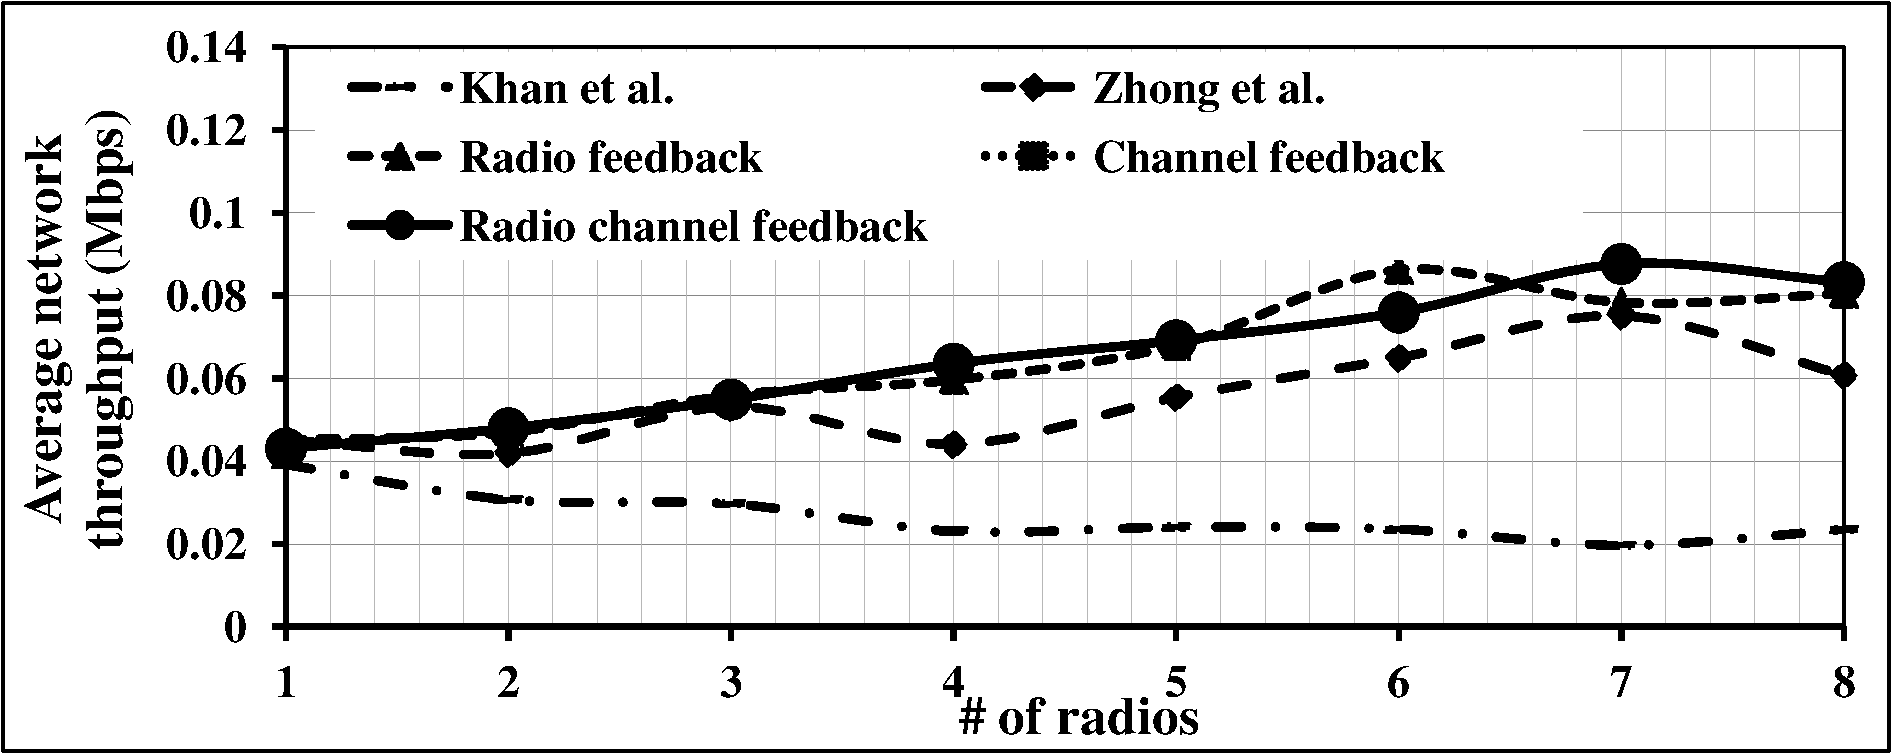
\includegraphics[width=\textwidth]{topology4/Throughput24d1}
        \caption{1Mbps application data rate}
        \label{fig:topology4T1}
    \end{subfigure}
    ~
    \begin{subfigure}[t]{0.45\textwidth}
        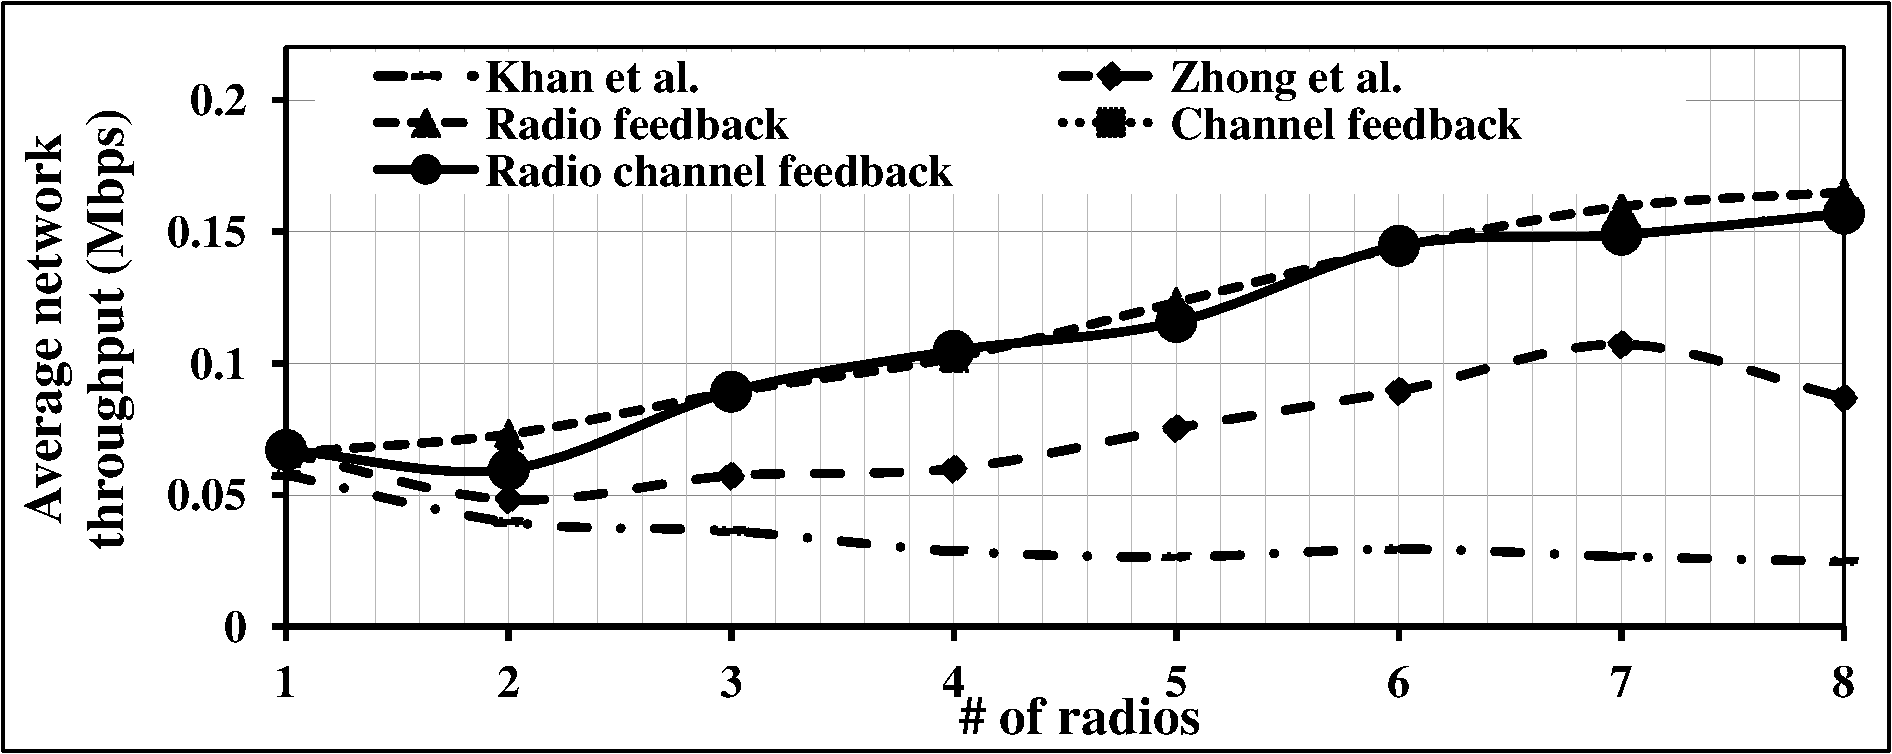
\includegraphics[width=\textwidth]{topology4/Throughput24d2}
        \caption{2Mbps application data rate}
        \label{fig:topology4T2}
    \end{subfigure}
    ~\\
    \begin{subfigure}[t]{0.45\textwidth}
        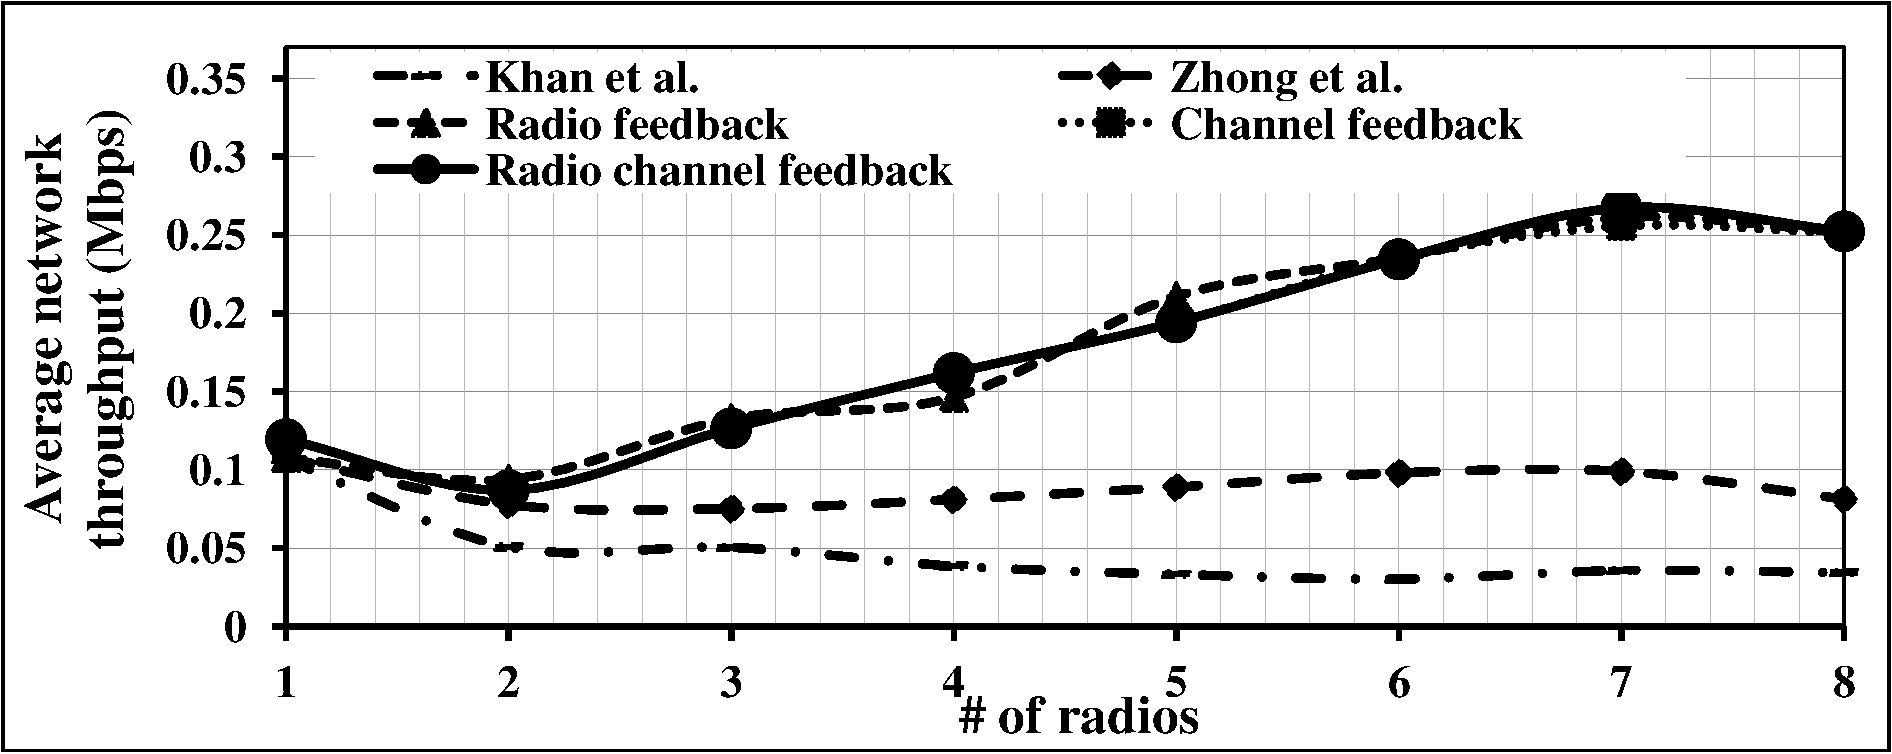
\includegraphics[width=\textwidth]{topology4/Throughput24d4}
        \caption{4Mbps application data rate}
        \label{fig:topology4T3}
    \end{subfigure}
    ~
    \begin{subfigure}[t]{0.45\textwidth}
        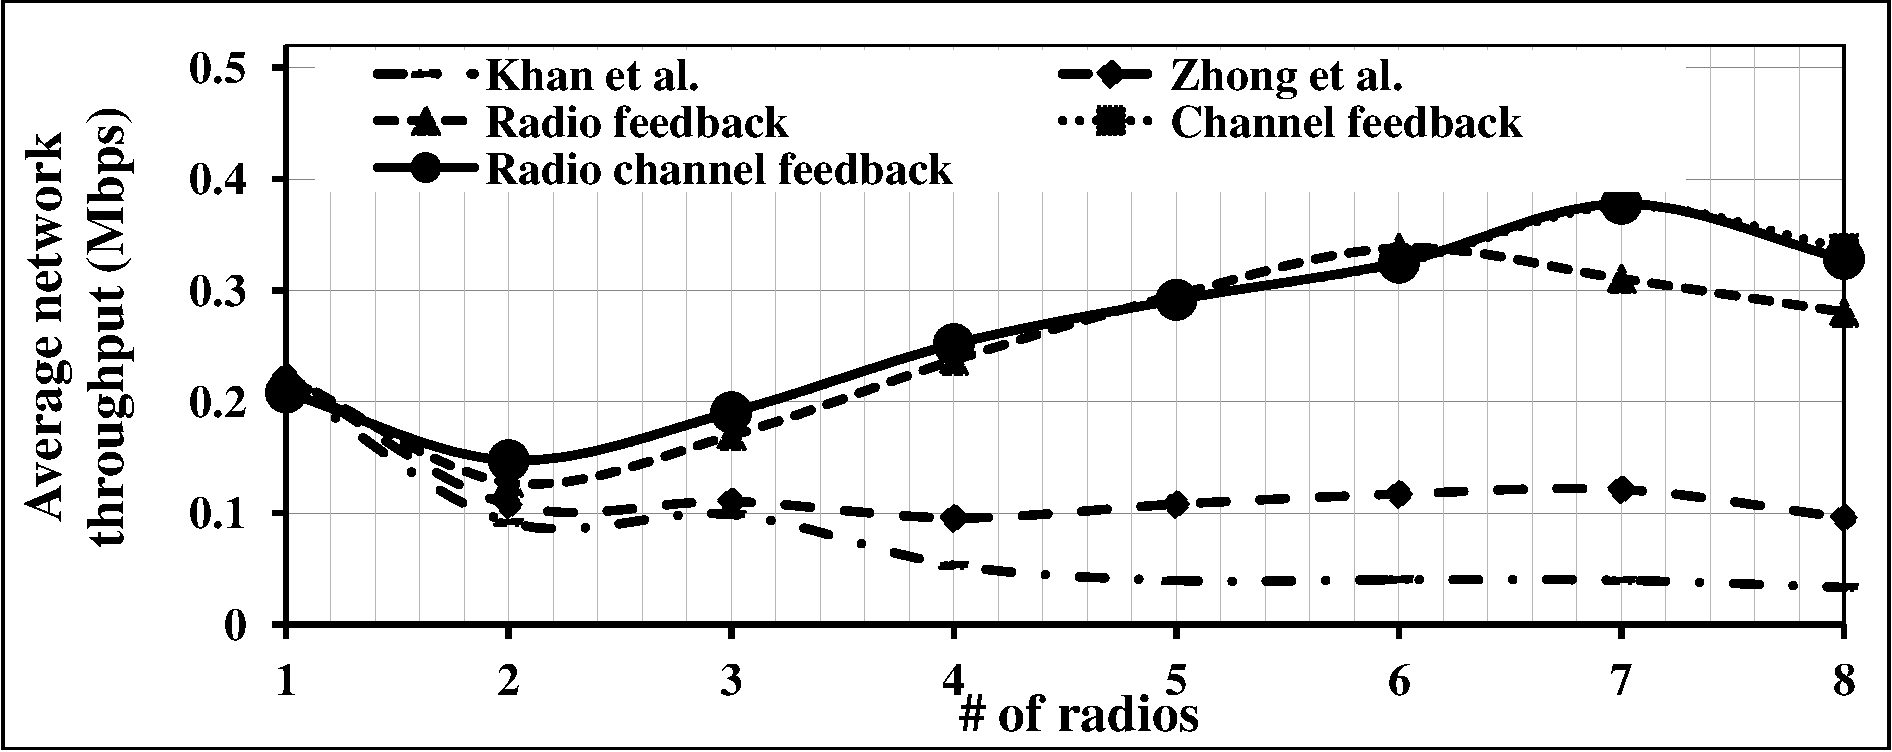
\includegraphics[width=\textwidth]{topology4/Throughput24d8}
        \caption{8Mbps application data rate}
        \label{fig:topology4T4}
    \end{subfigure}
    ~\\
    \begin{subfigure}[t]{0.45\textwidth}
        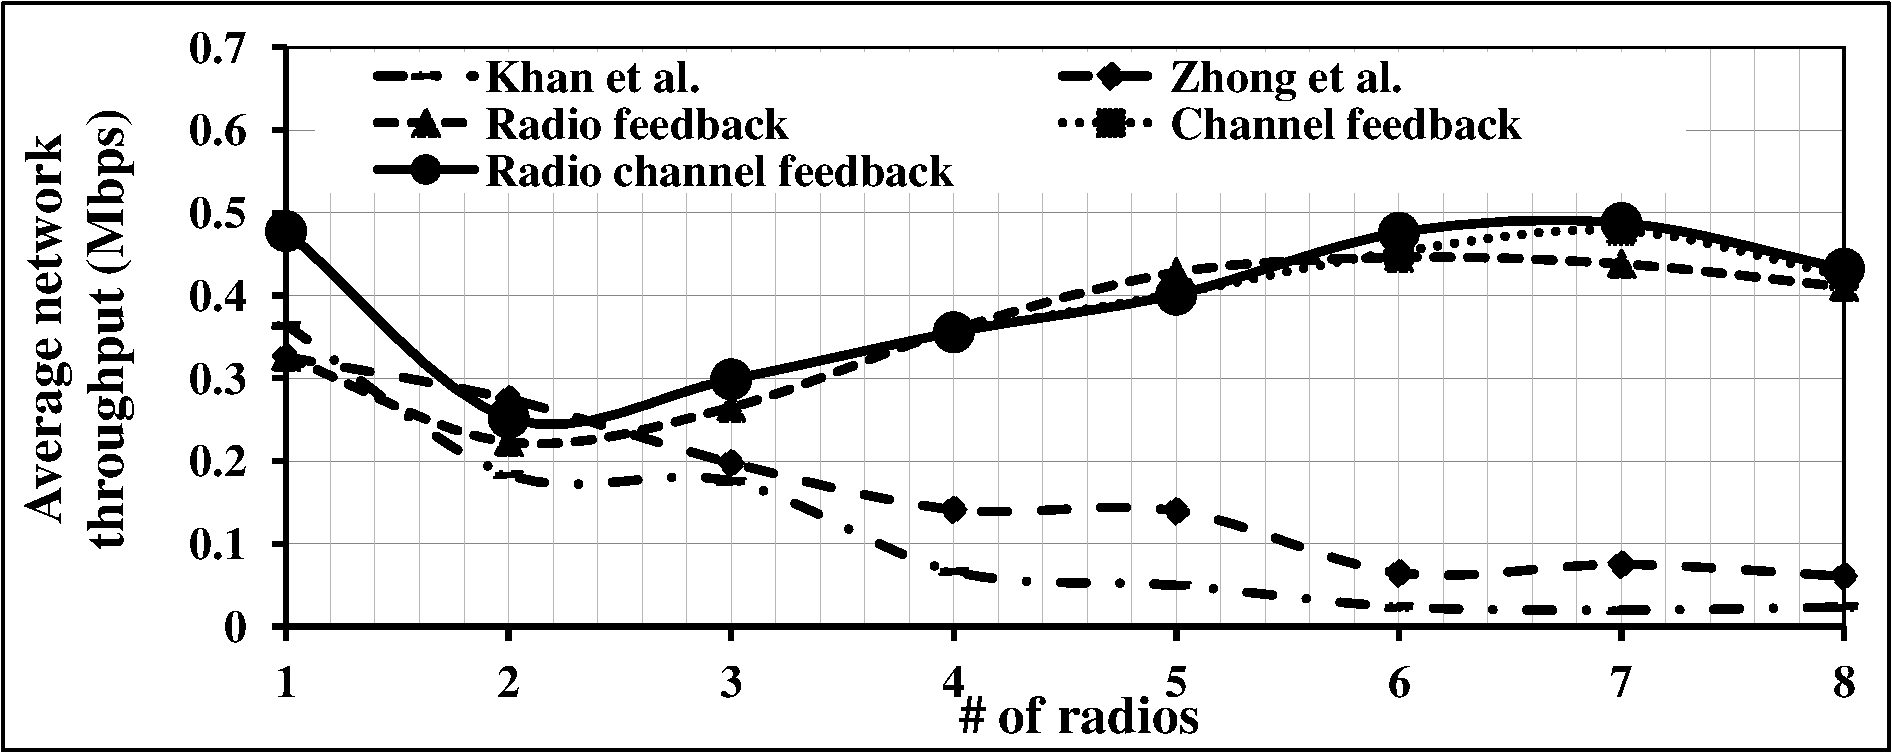
\includegraphics[width=\textwidth]{topology4/Throughput24d16}
        \caption{16Mbps application data rate}
        \label{fig:topology4T5}
    \end{subfigure}
    ~
    \begin{subfigure}[t]{0.45\textwidth}
        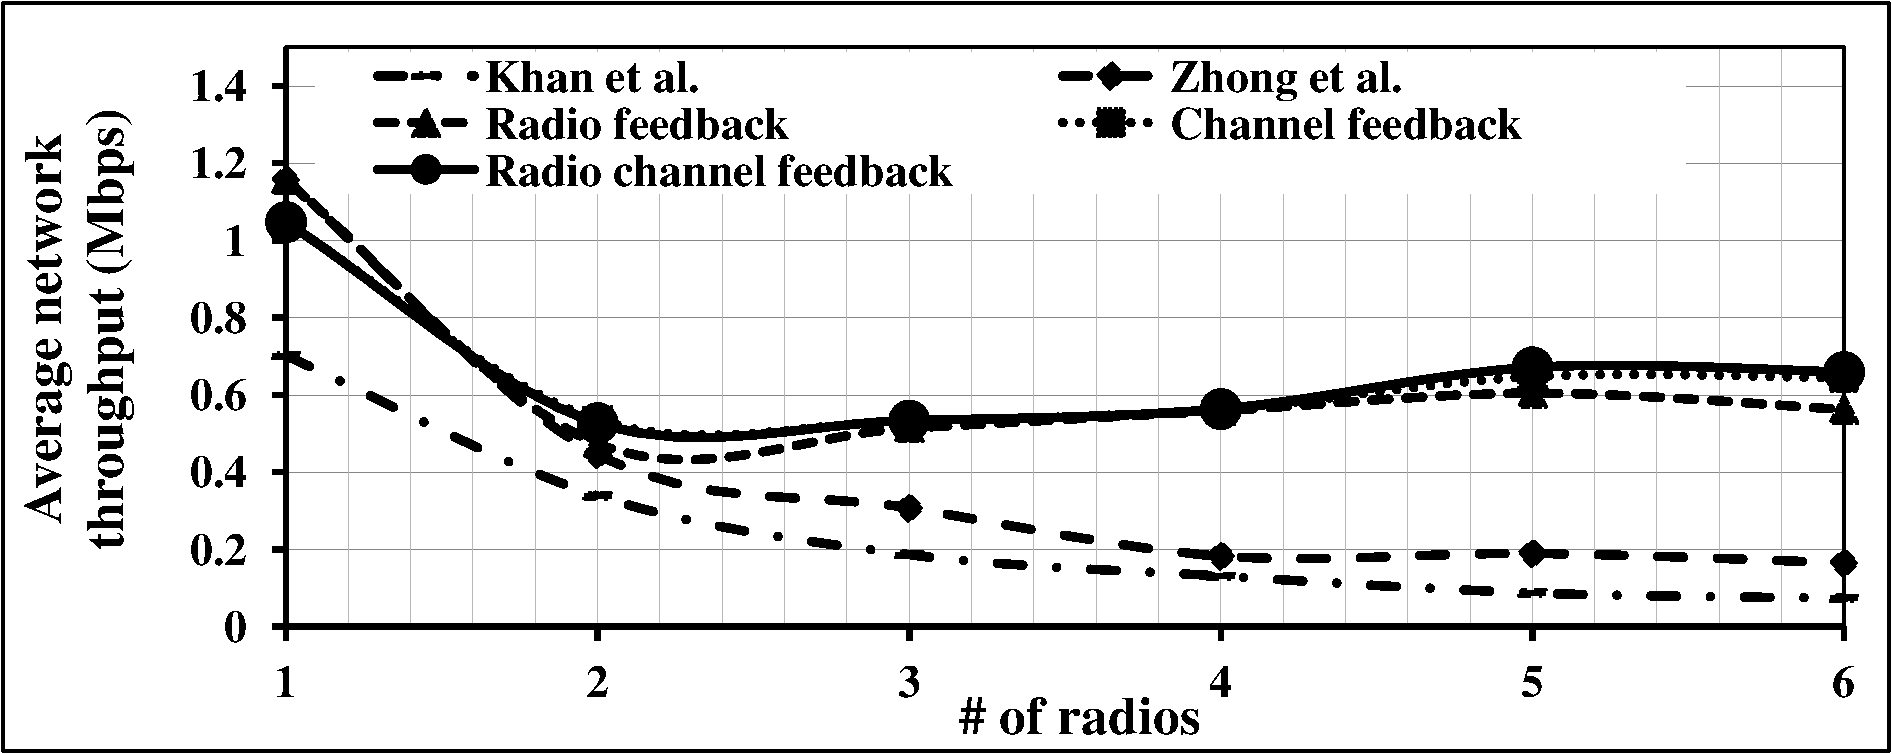
\includegraphics[width=\textwidth]{topology4/Throughput24d32}
        \caption{32Mbps application data rate}
        \label{fig:topology4T6}
    \end{subfigure}
    \caption{Average network throughput with varying number of radios for various application data rates}
    \label{fig:topology4T}
\end{figure*}

\begin{figure*}[!htbp]
    \centering
    \begin{subfigure}[t]{0.45\textwidth}
        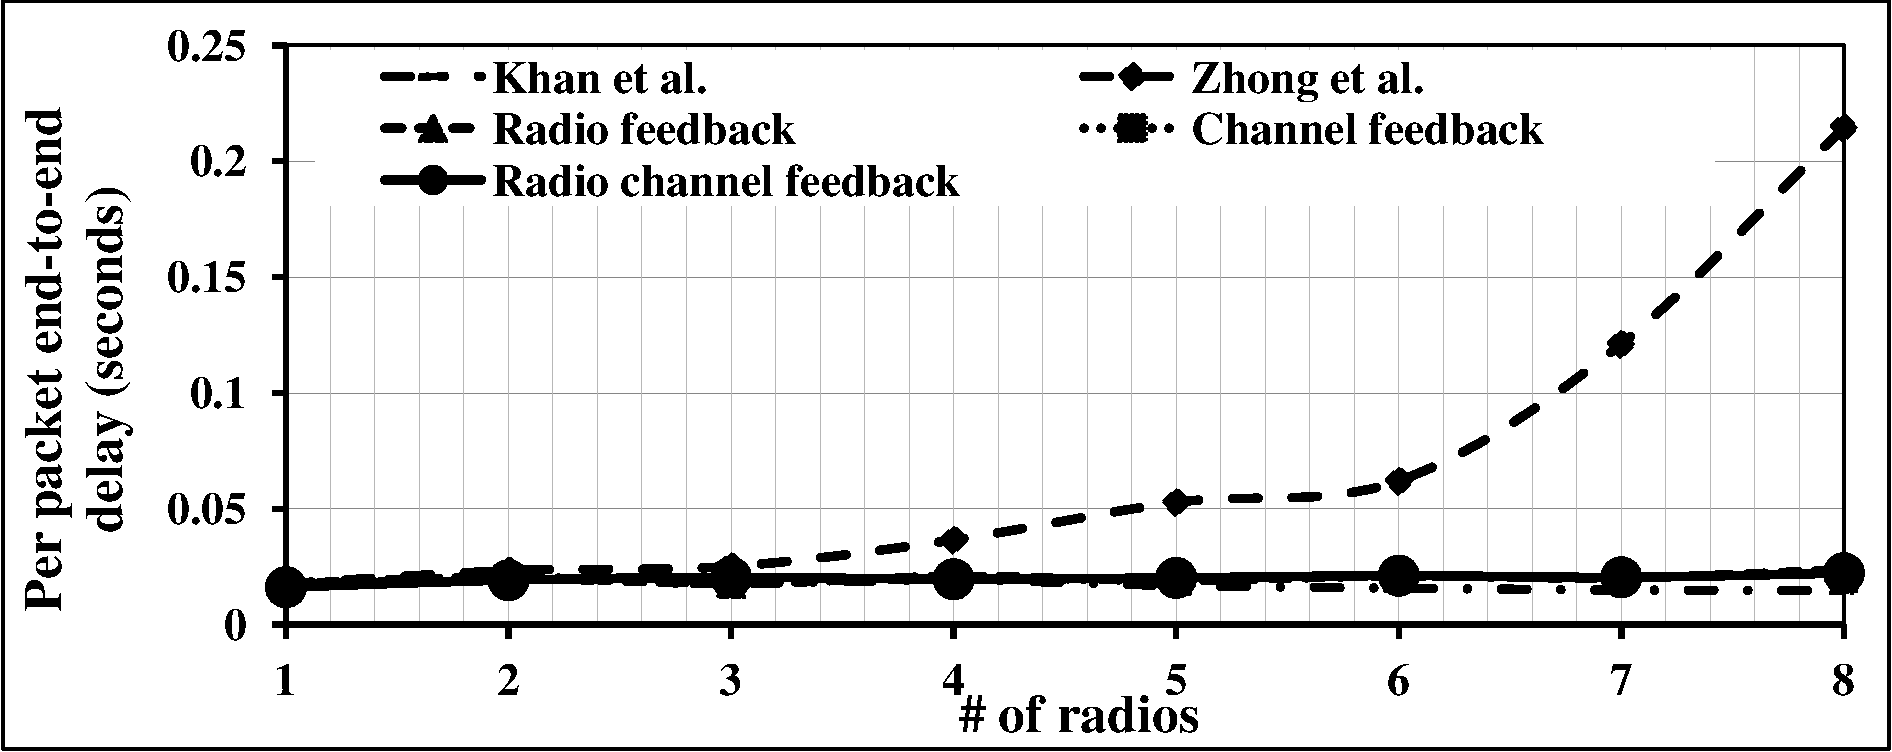
\includegraphics[width=\textwidth]{topology4/Delay24d1}
        \caption{1Mbps application data rate}
        \label{fig:topology4D1}
    \end{subfigure}
    ~
    \begin{subfigure}[t]{0.45\textwidth}
        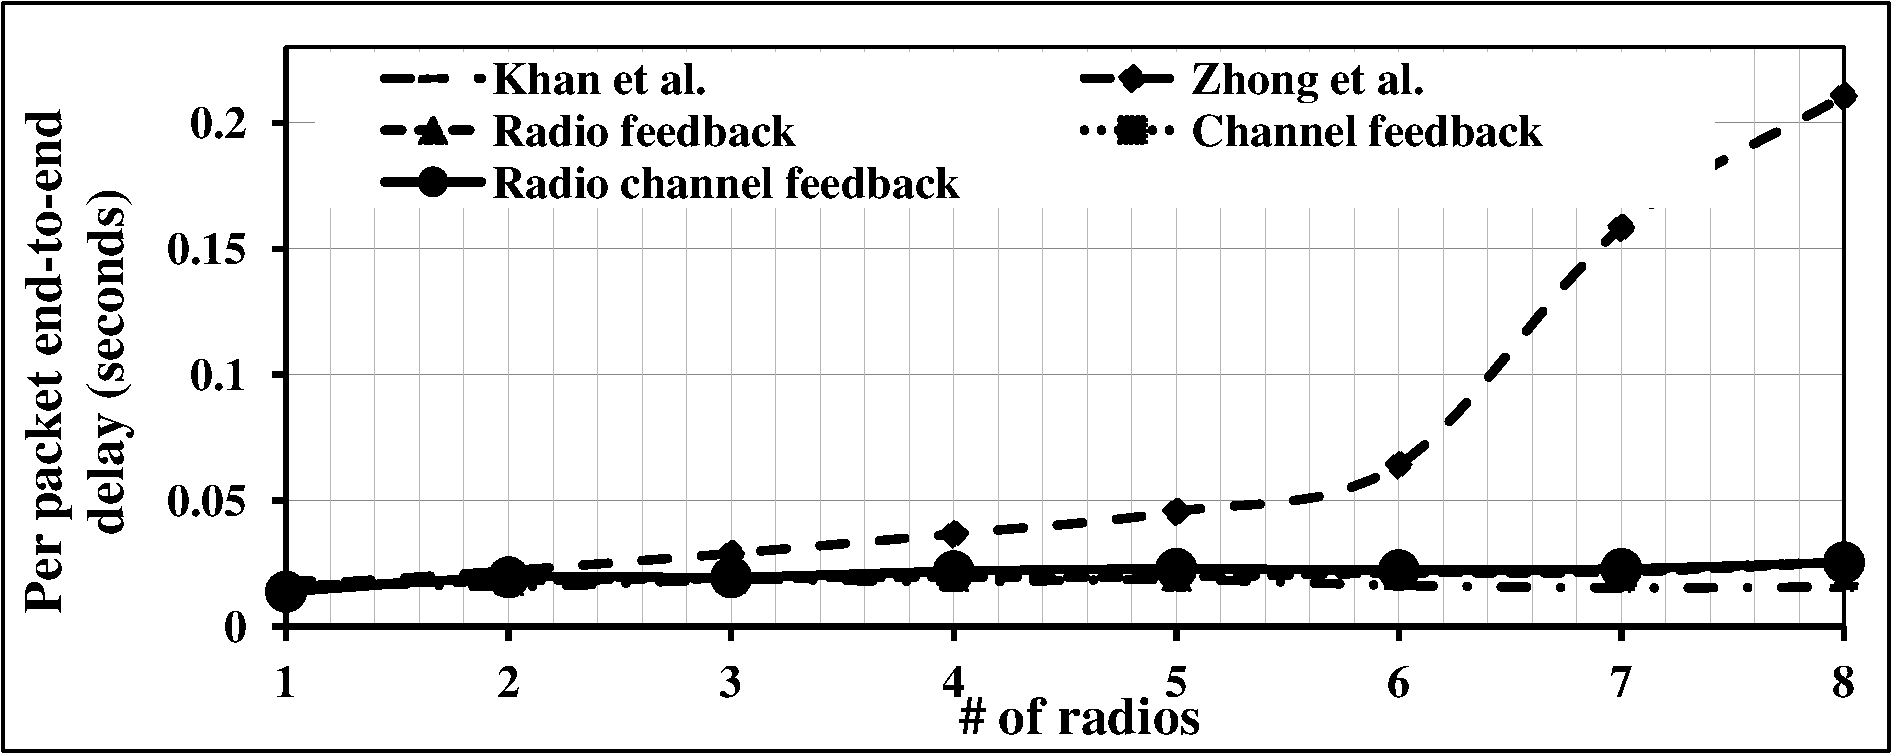
\includegraphics[width=\textwidth]{topology4/Delay24d2}
        \caption{2Mbps application data rate}
        \label{fig:topology4D2}
    \end{subfigure}
    ~\\
    \begin{subfigure}[t]{0.45\textwidth}
        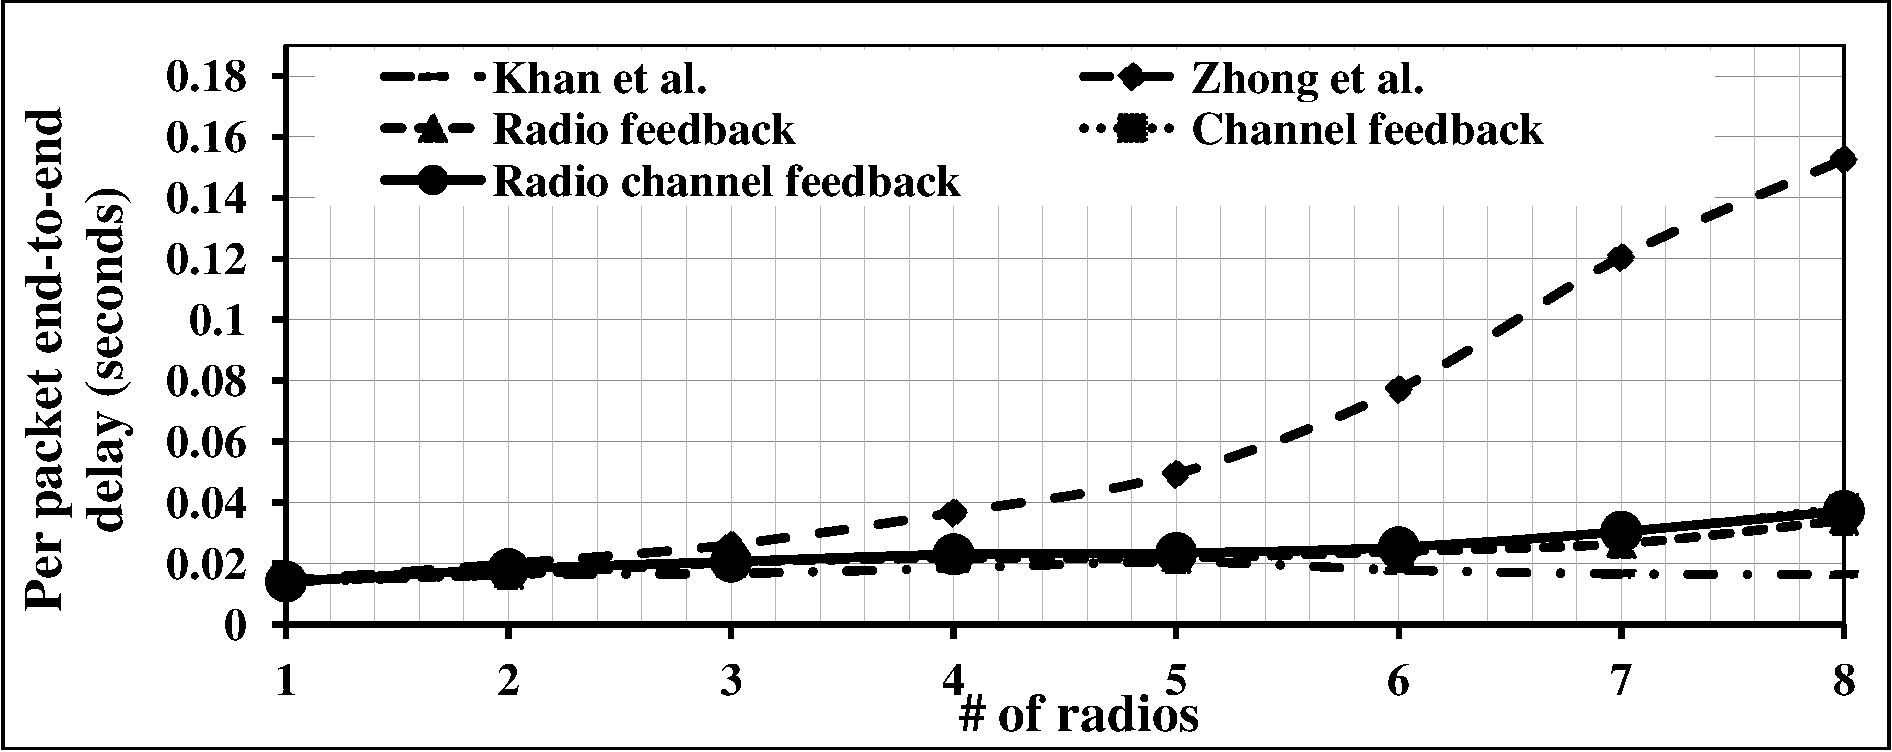
\includegraphics[width=\textwidth]{topology4/Delay24d4}
        \caption{4Mbps application data rate}
        \label{fig:topology4D3}
    \end{subfigure}
    ~
    \begin{subfigure}[t]{0.45\textwidth}
        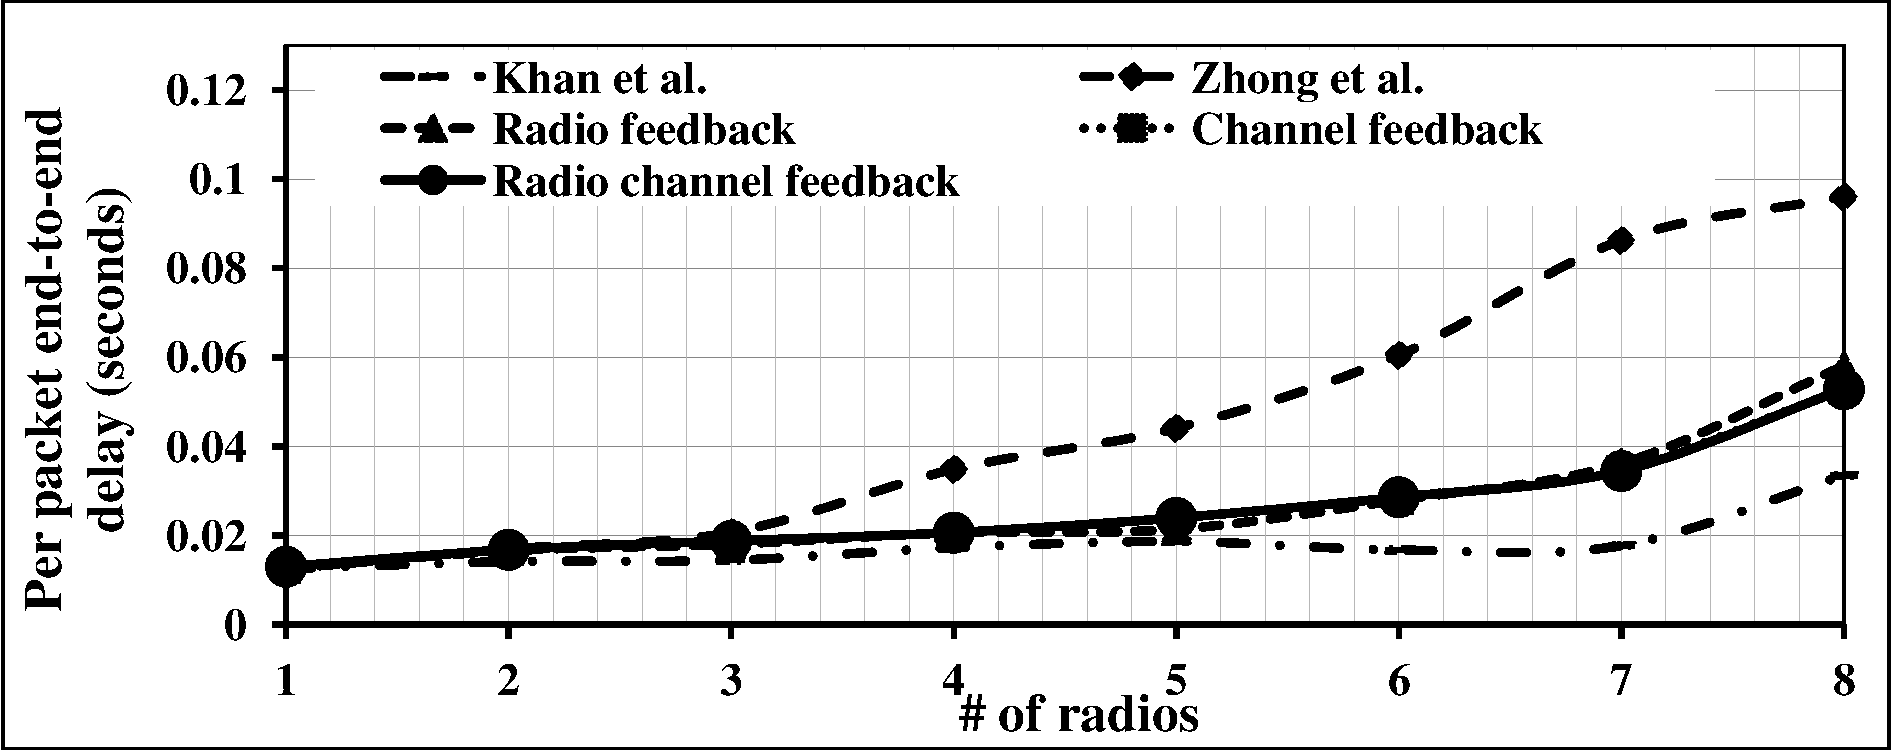
\includegraphics[width=\textwidth]{topology4/Delay24d8}
        \caption{8Mbps application data rate}
        \label{fig:topology4D4}
    \end{subfigure}
    ~\\
    \begin{subfigure}[t]{0.45\textwidth}
        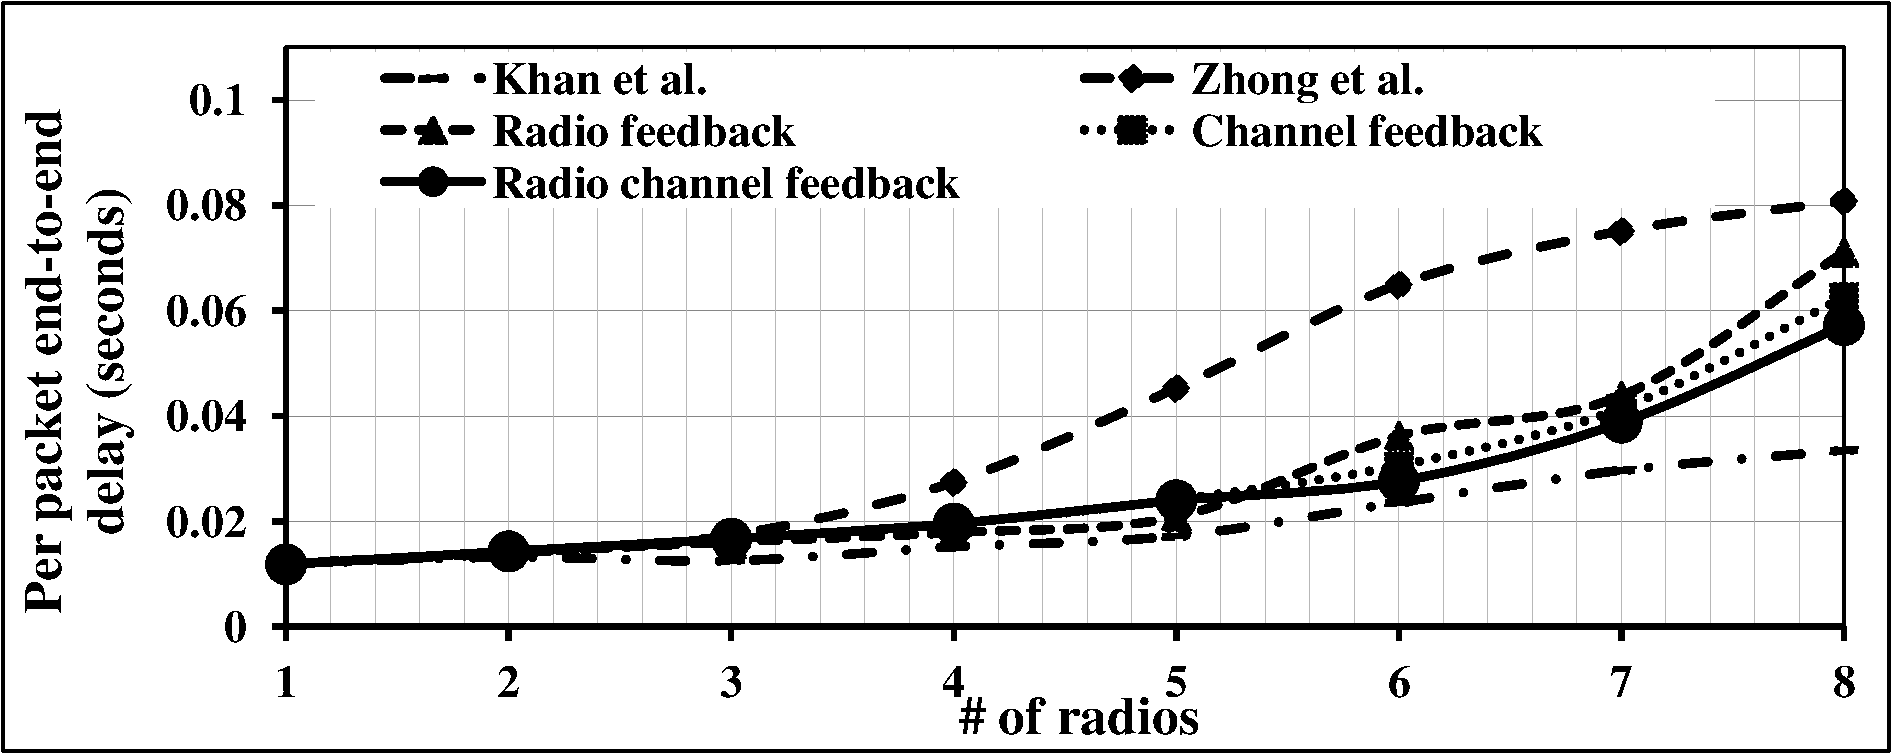
\includegraphics[width=\textwidth]{topology4/Delay24d16}
        \caption{16Mbps application data rate}
        \label{fig:topology4D5}
    \end{subfigure}
    ~
    \begin{subfigure}[t]{0.45\textwidth}
        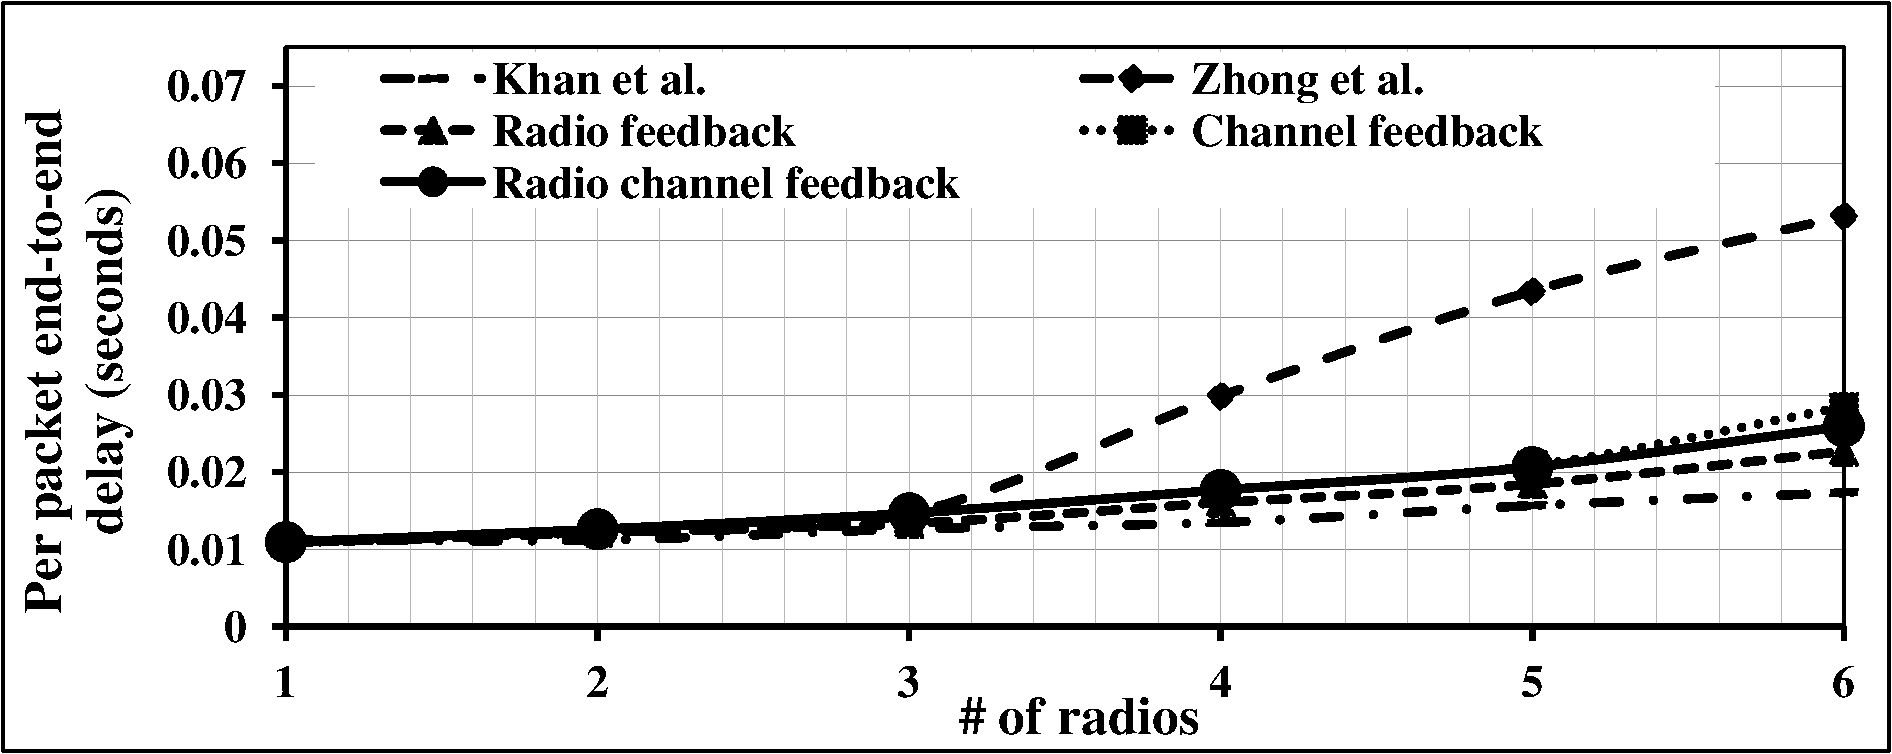
\includegraphics[width=\textwidth]{topology4/Delay24d32}
        \caption{32Mbps application data rate}
        \label{fig:topology4D6}
    \end{subfigure}
    \caption{Average end-to-end delay with varying number of radios for various application data rates}
    \label{fig:topology4D}
\end{figure*}

\begin{landscape}
\begin{figure*}[!htbp]
    \centering
    \begin{subfigure}[t]{0.625\textwidth}
        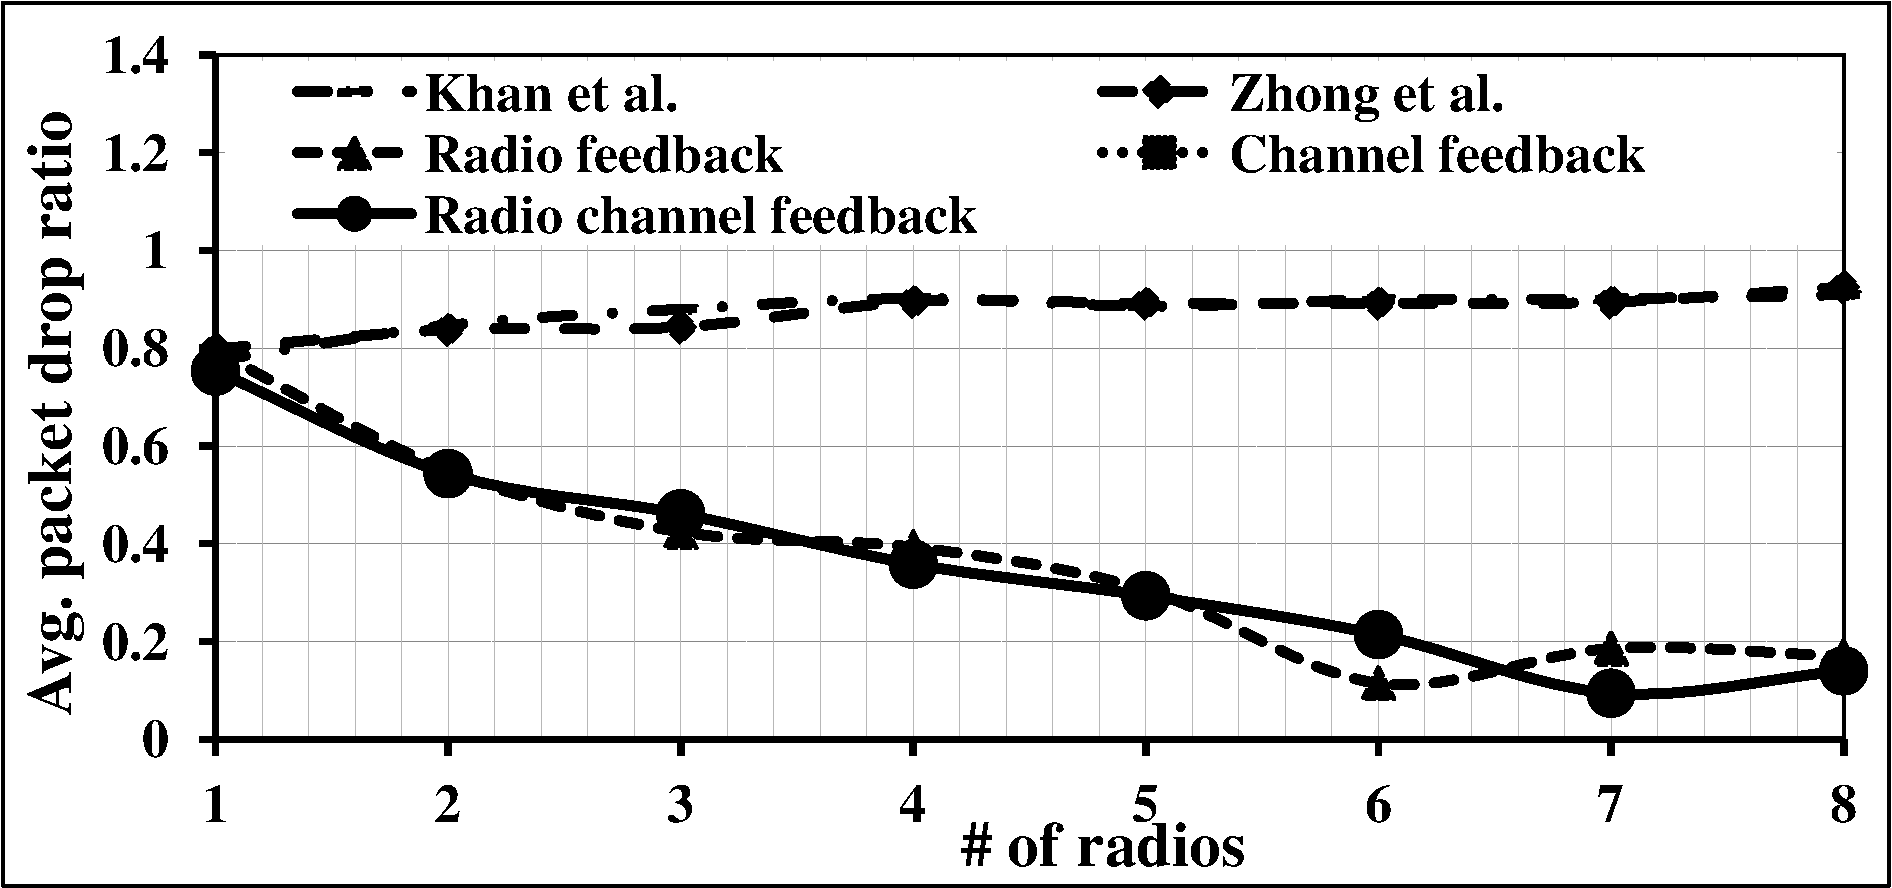
\includegraphics[width=\textwidth]{topology4/PacketDropRatio24d1}
        \caption{1Mbps application data rate}
        \label{fig:topology4P1}
    \end{subfigure}
    ~
    \begin{subfigure}[t]{0.625\textwidth}
        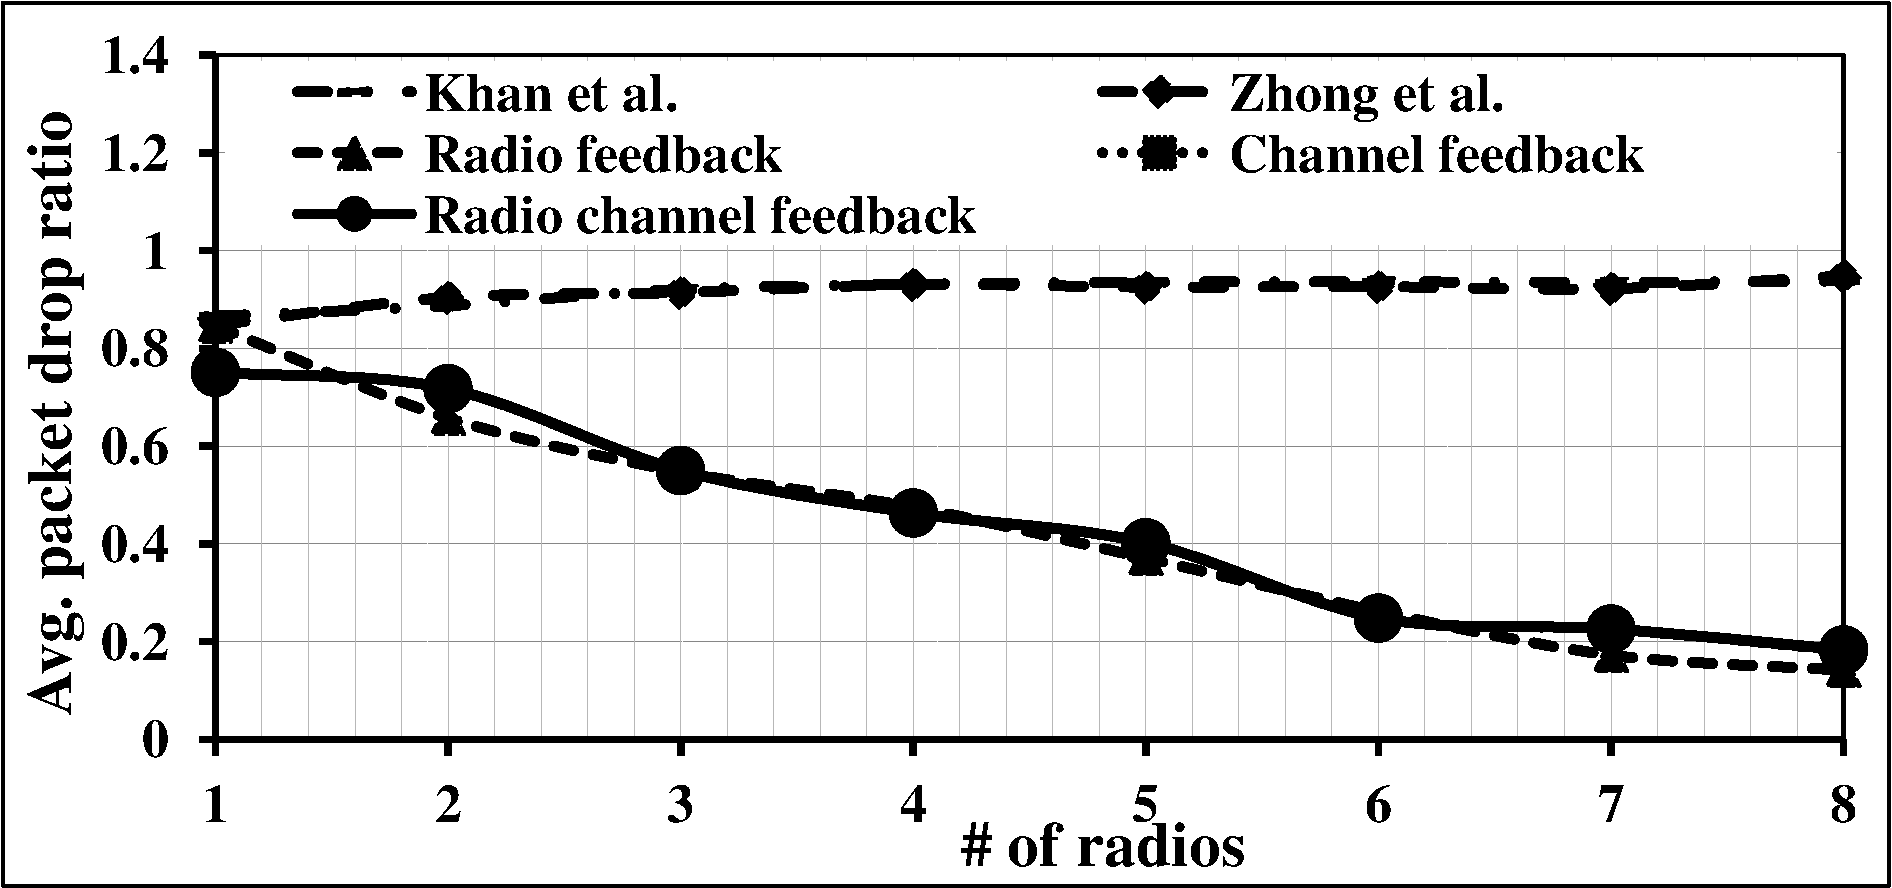
\includegraphics[width=\textwidth]{topology4/PacketDropRatio24d2}
        \caption{2Mbps application data rate}
        \label{fig:topology4P2}
    \end{subfigure}
    ~\\
    \begin{subfigure}[t]{0.625\textwidth}
        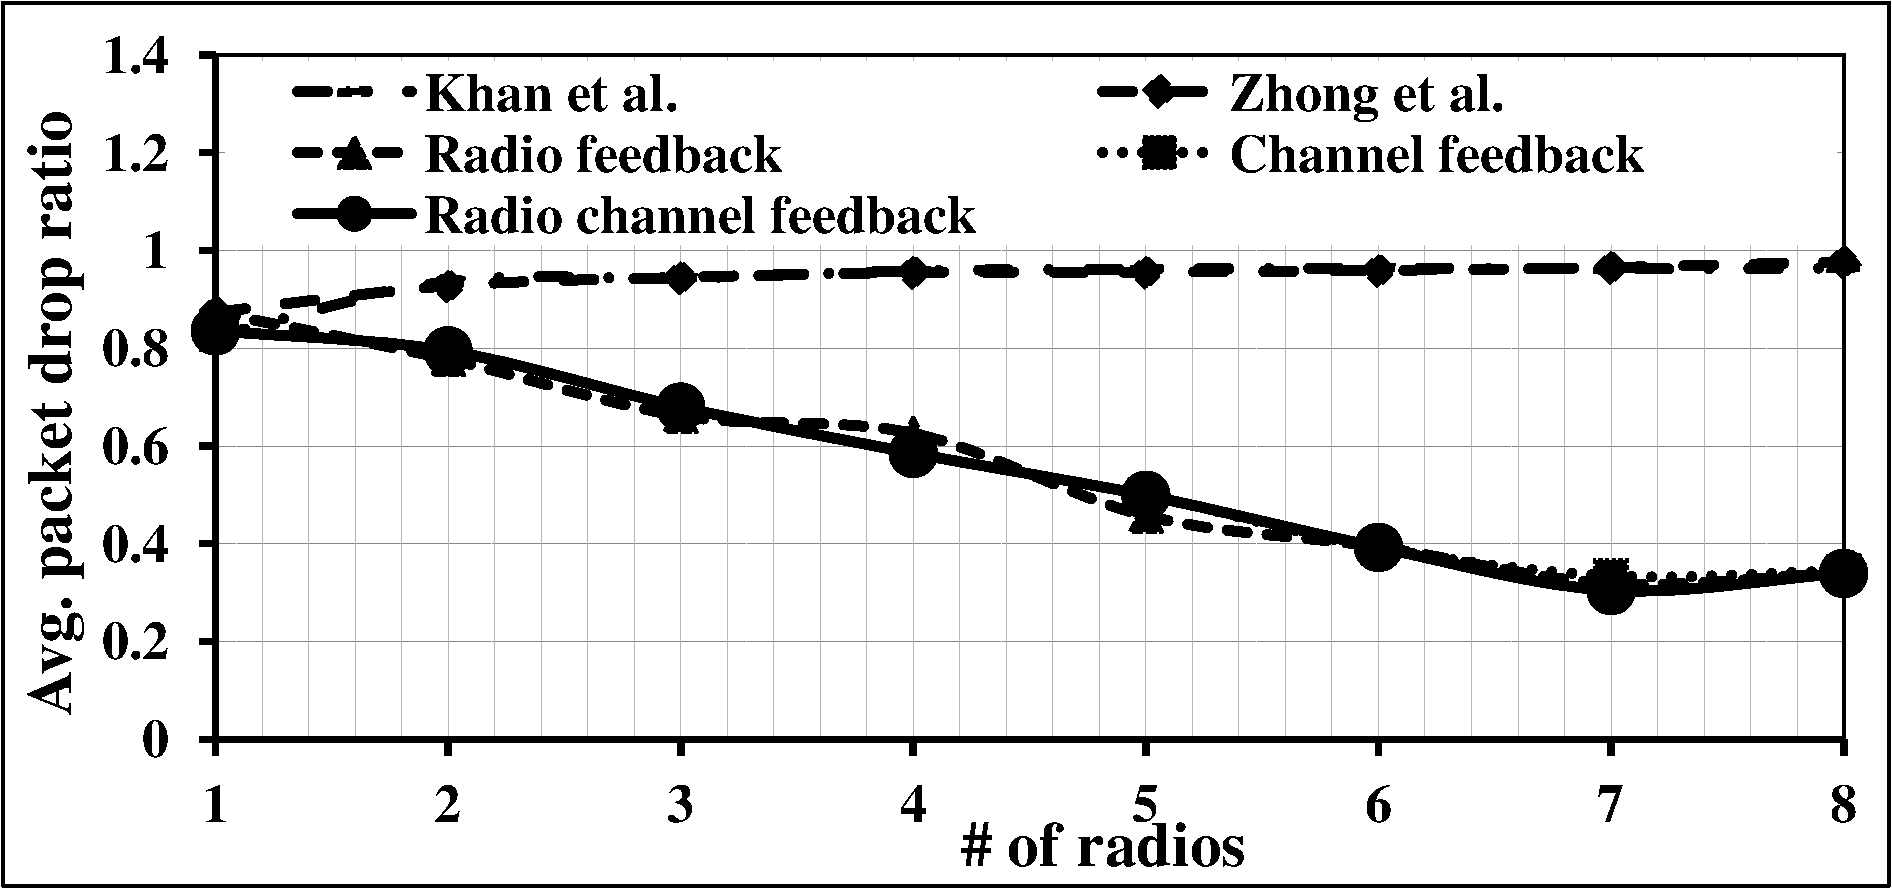
\includegraphics[width=\textwidth]{topology4/PacketDropRatio24d4}
        \caption{4Mbps application data rate}
        \label{fig:topology4P3}
    \end{subfigure}
    ~
    \begin{subfigure}[t]{0.625\textwidth}
        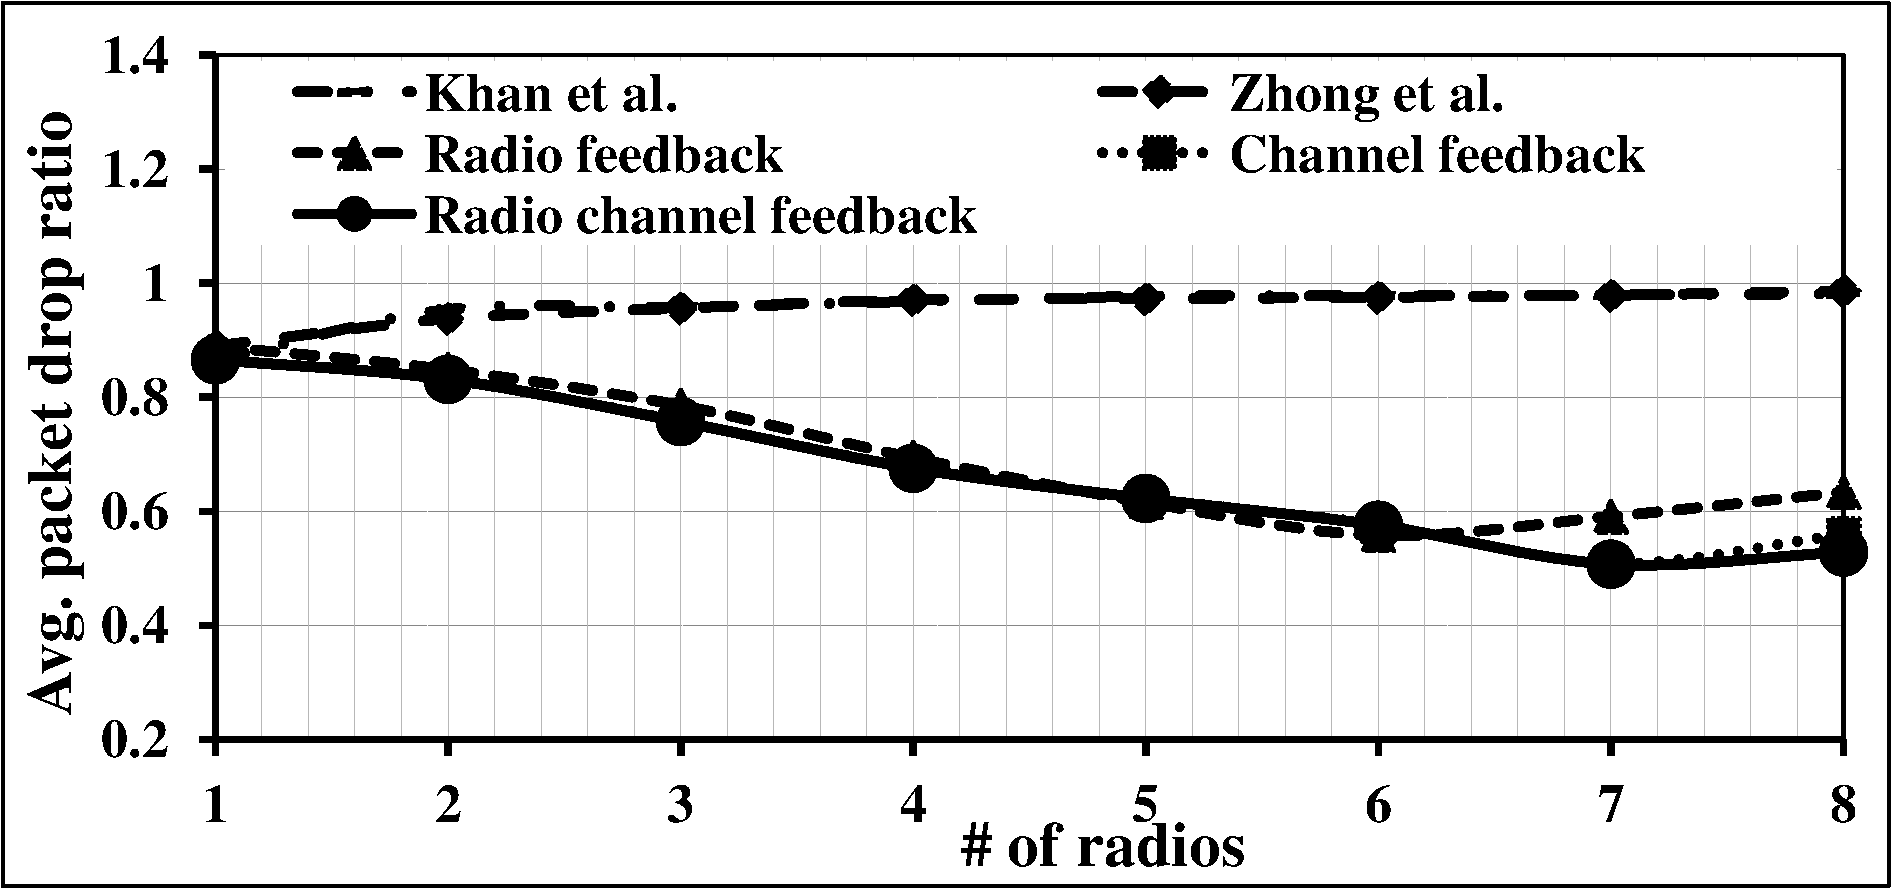
\includegraphics[width=\textwidth]{topology4/PacketDropRatio24d8}
        \caption{8Mbps application data rate}
        \label{fig:topology4P4}
    \end{subfigure}
    ~\\
    \begin{subfigure}[t]{0.625\textwidth}
        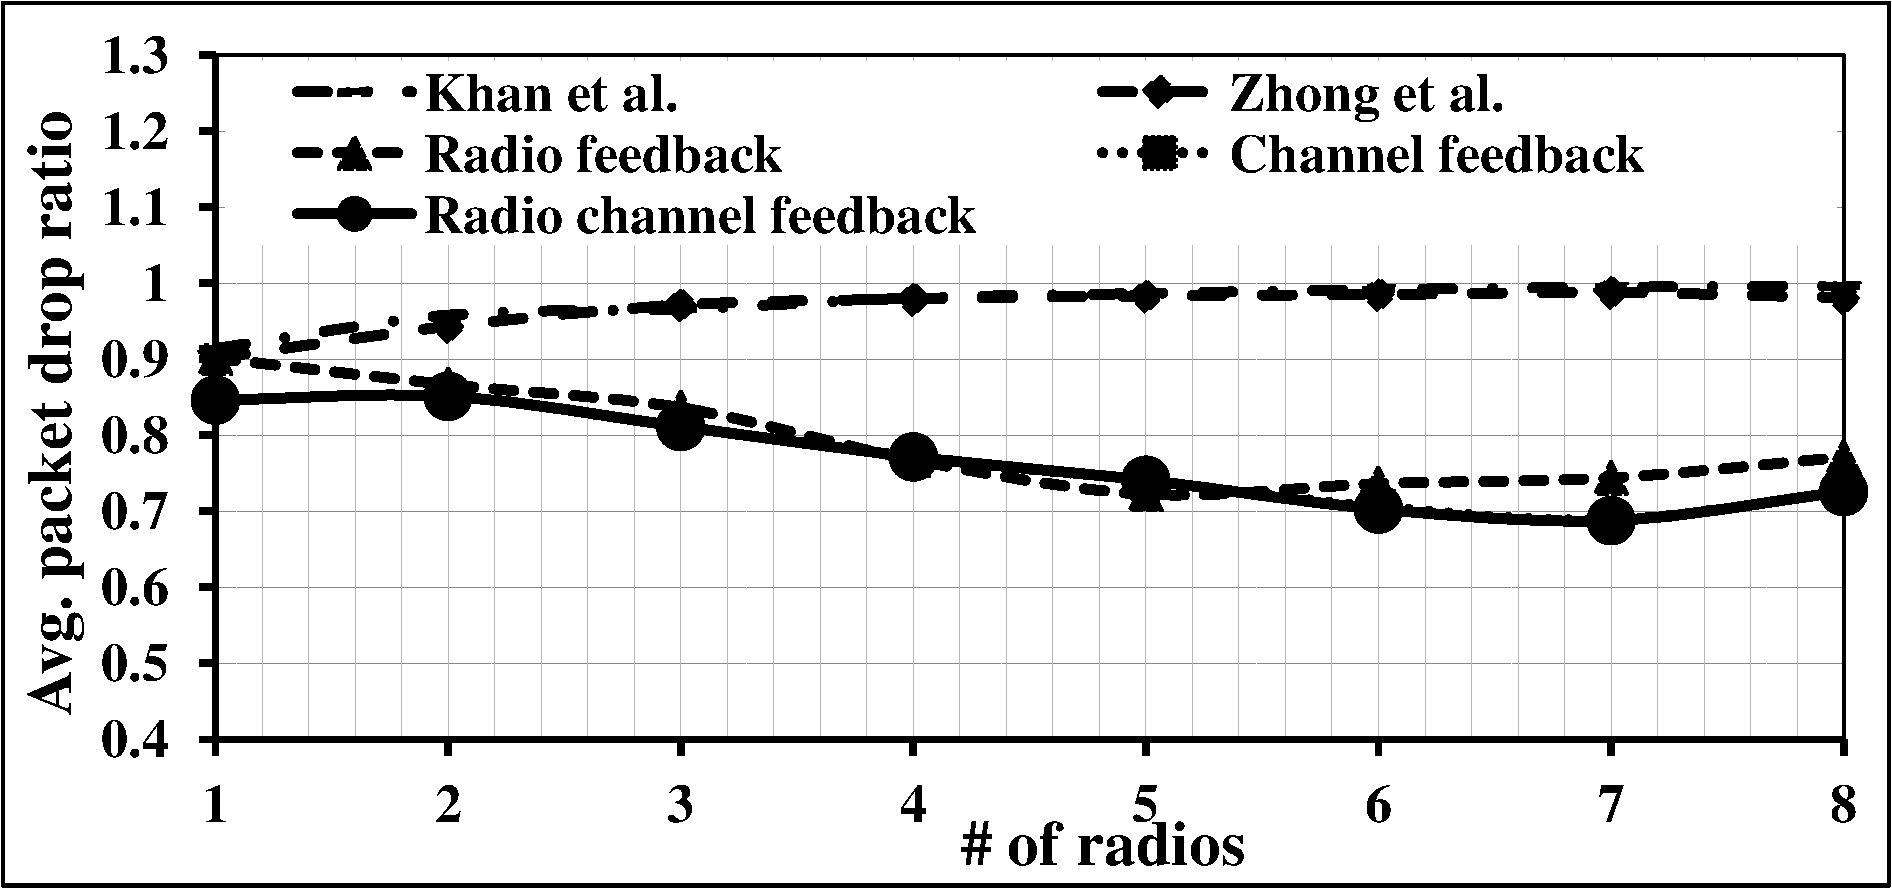
\includegraphics[width=\textwidth]{topology4/PacketDropRatio24d16}
        \caption{16Mbps application data rate}
        \label{fig:topology4P5}
    \end{subfigure}
    ~
    \begin{subfigure}[t]{0.625\textwidth}
        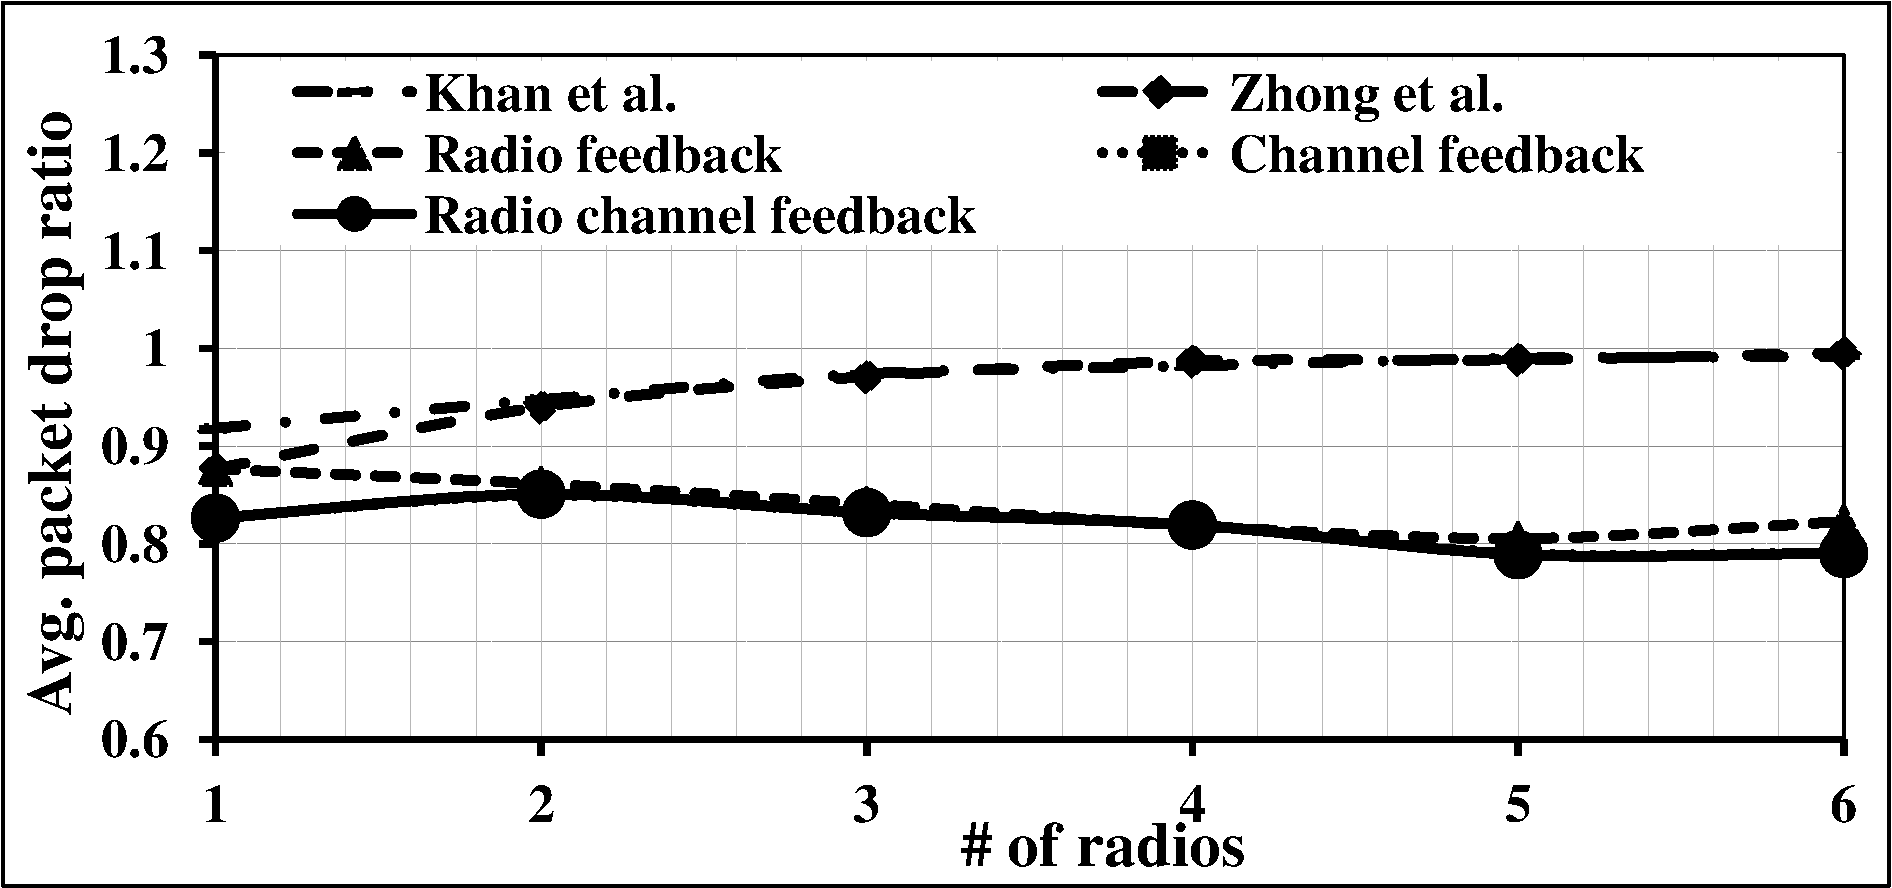
\includegraphics[width=\textwidth]{topology4/PacketDropRatio24d32}
        \caption{32Mbps application data rate}
        \label{fig:topology4P6}
    \end{subfigure}
    \caption{Average packet drop ratio with varying number of radios for various application data rates}
    \label{fig:topology4P}
\end{figure*}
\end{landscape}

\begin{figure*}[!htbp]
    \centering
    \begin{subfigure}[t]{0.45\textwidth}
        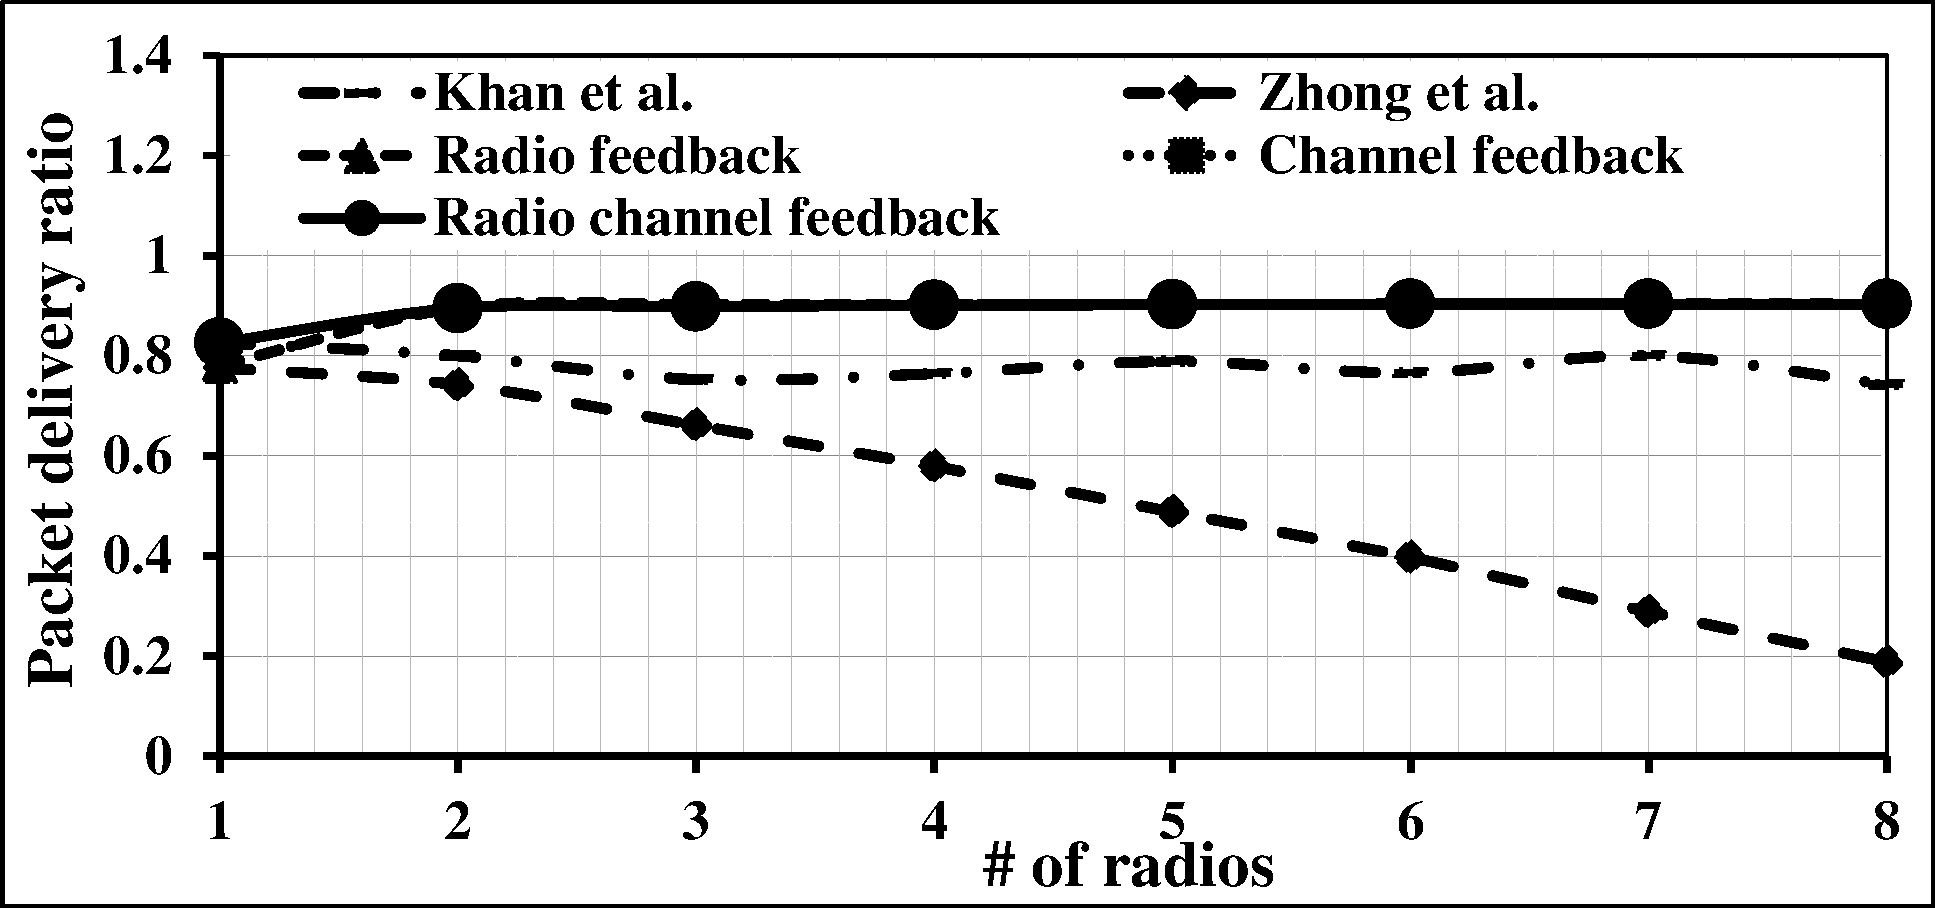
\includegraphics[width=\textwidth]{topology4/DeliveryRatio24d1}
        \caption{1Mbps application data rate}
        \label{fig:topology4PD1}
    \end{subfigure}
    ~
    \begin{subfigure}[t]{0.45\textwidth}
        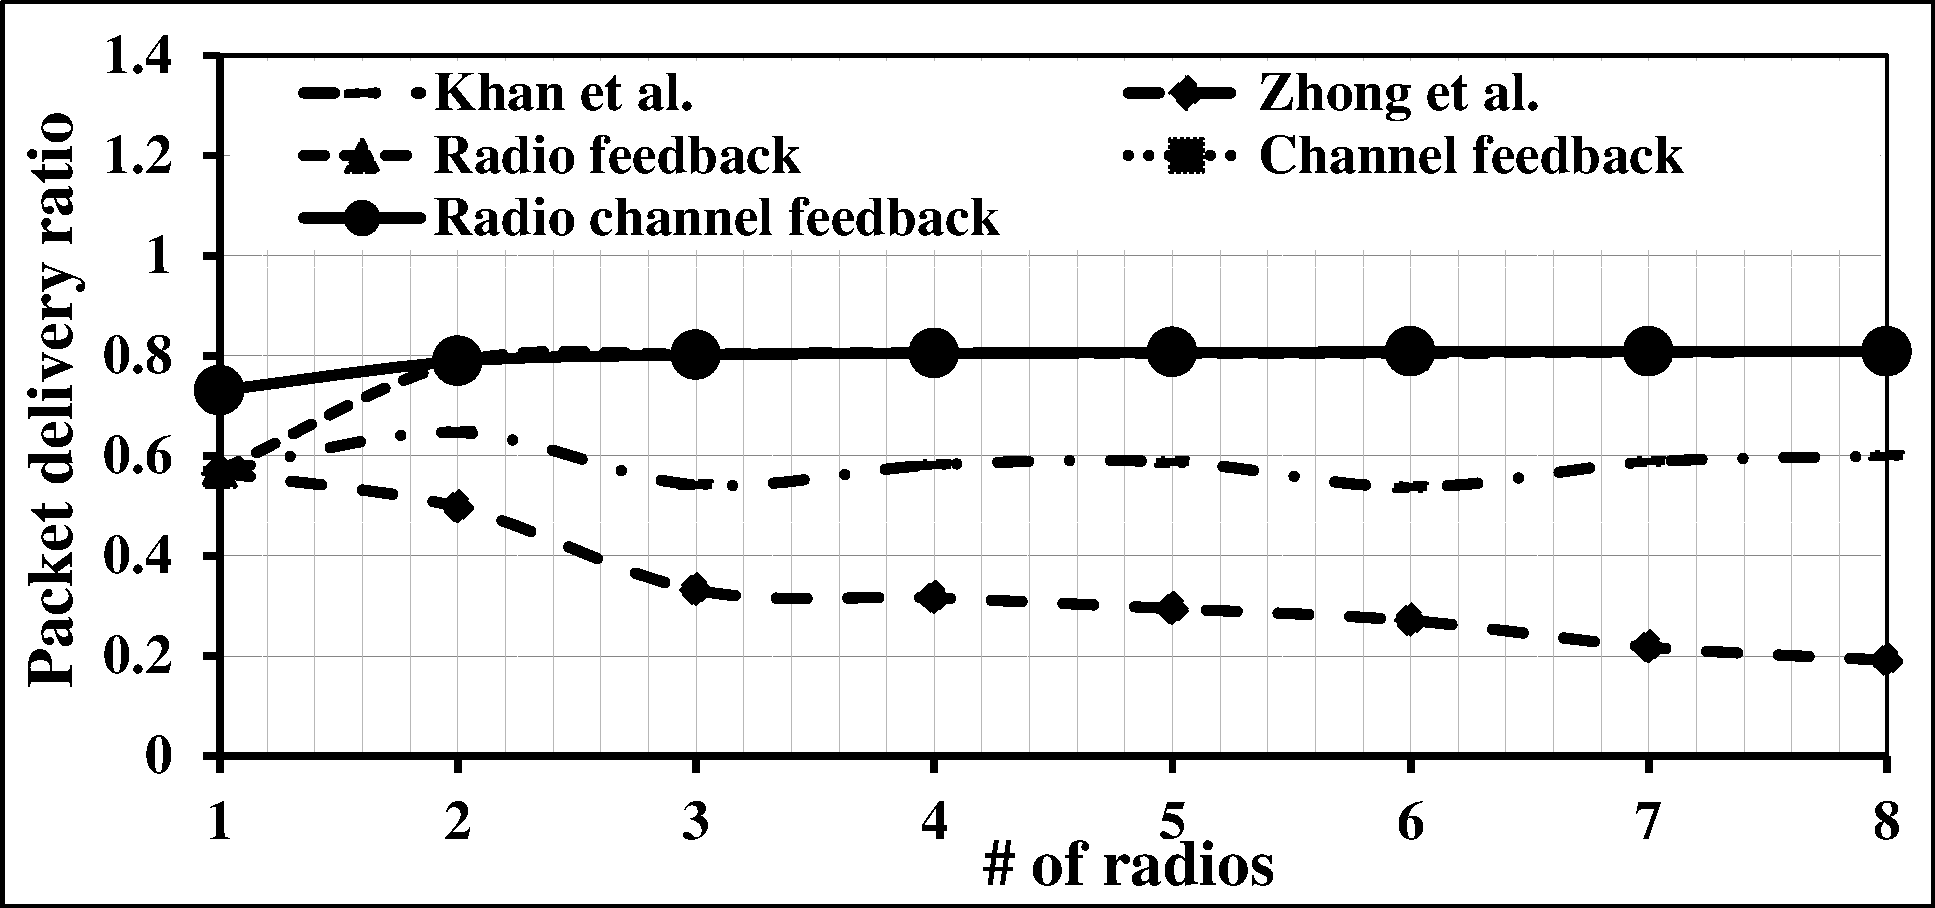
\includegraphics[width=\textwidth]{topology4/DeliveryRatio24d2}
        \caption{2Mbps application data rate}
        \label{fig:topology4PD2}
    \end{subfigure}
    ~\\
    \begin{subfigure}[t]{0.45\textwidth}
        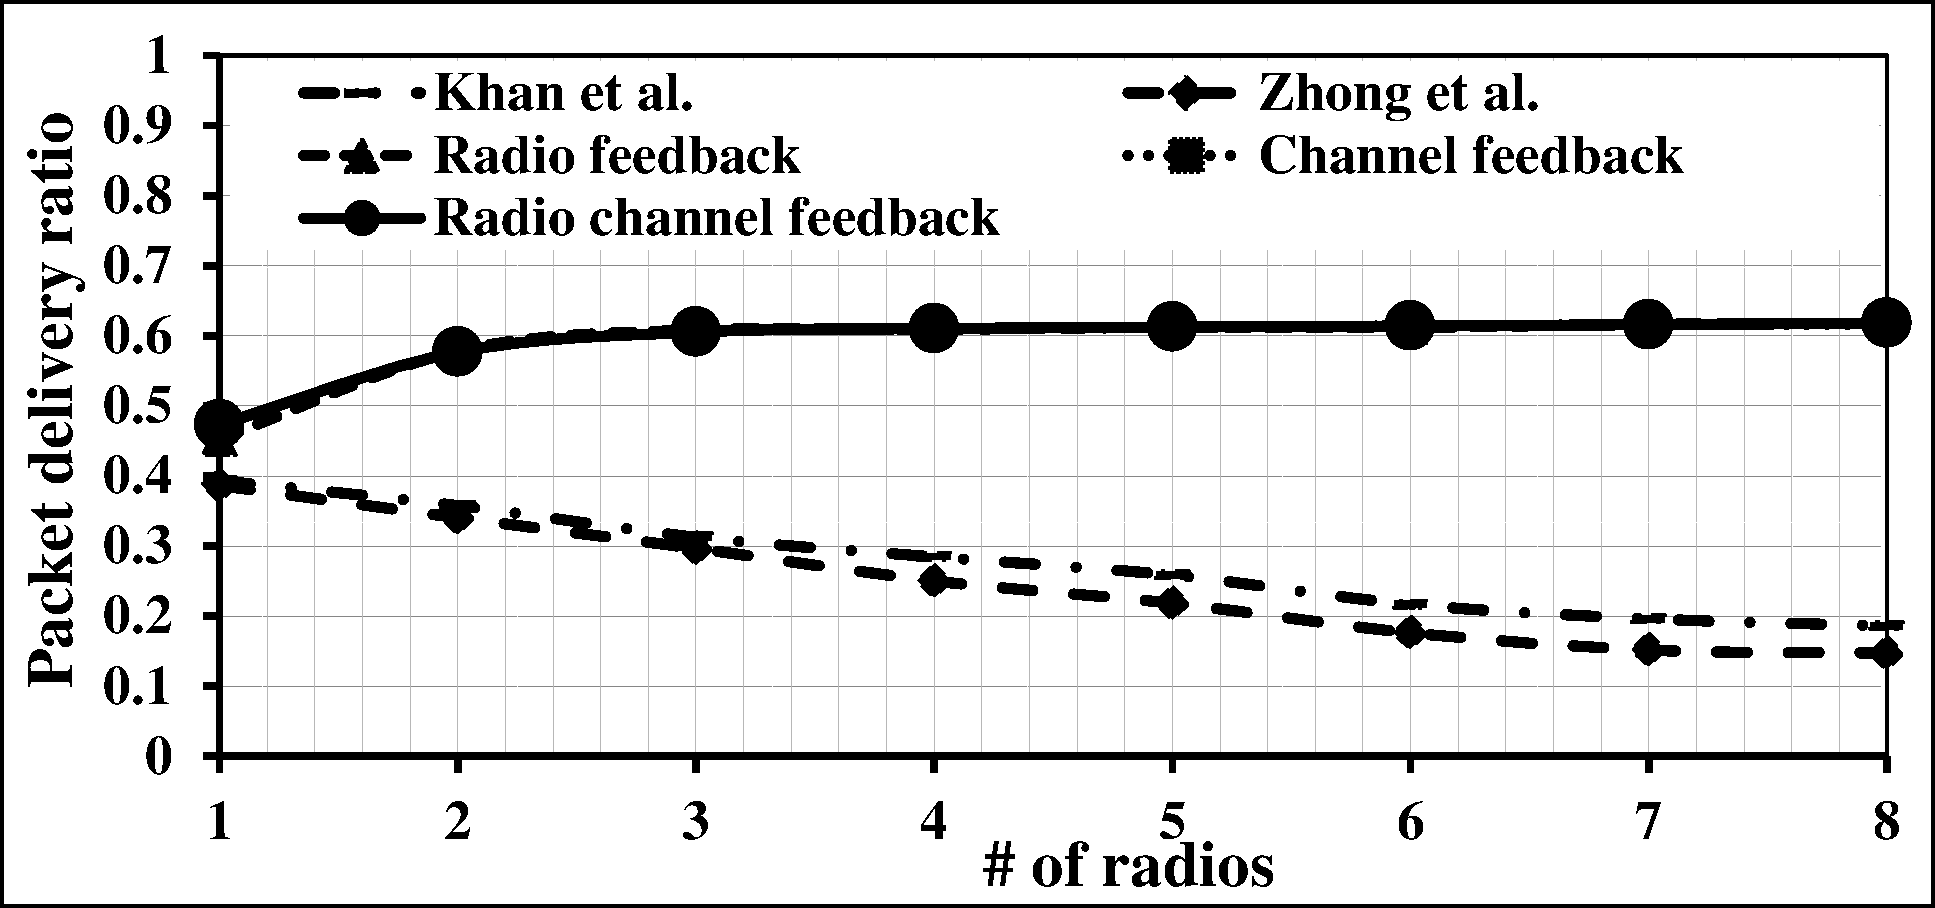
\includegraphics[width=\textwidth]{topology4/DeliveryRatio24d4}
        \caption{4Mbps application data rate}
        \label{fig:topology4PD3}
    \end{subfigure}
    ~
    \begin{subfigure}[t]{0.45\textwidth}
        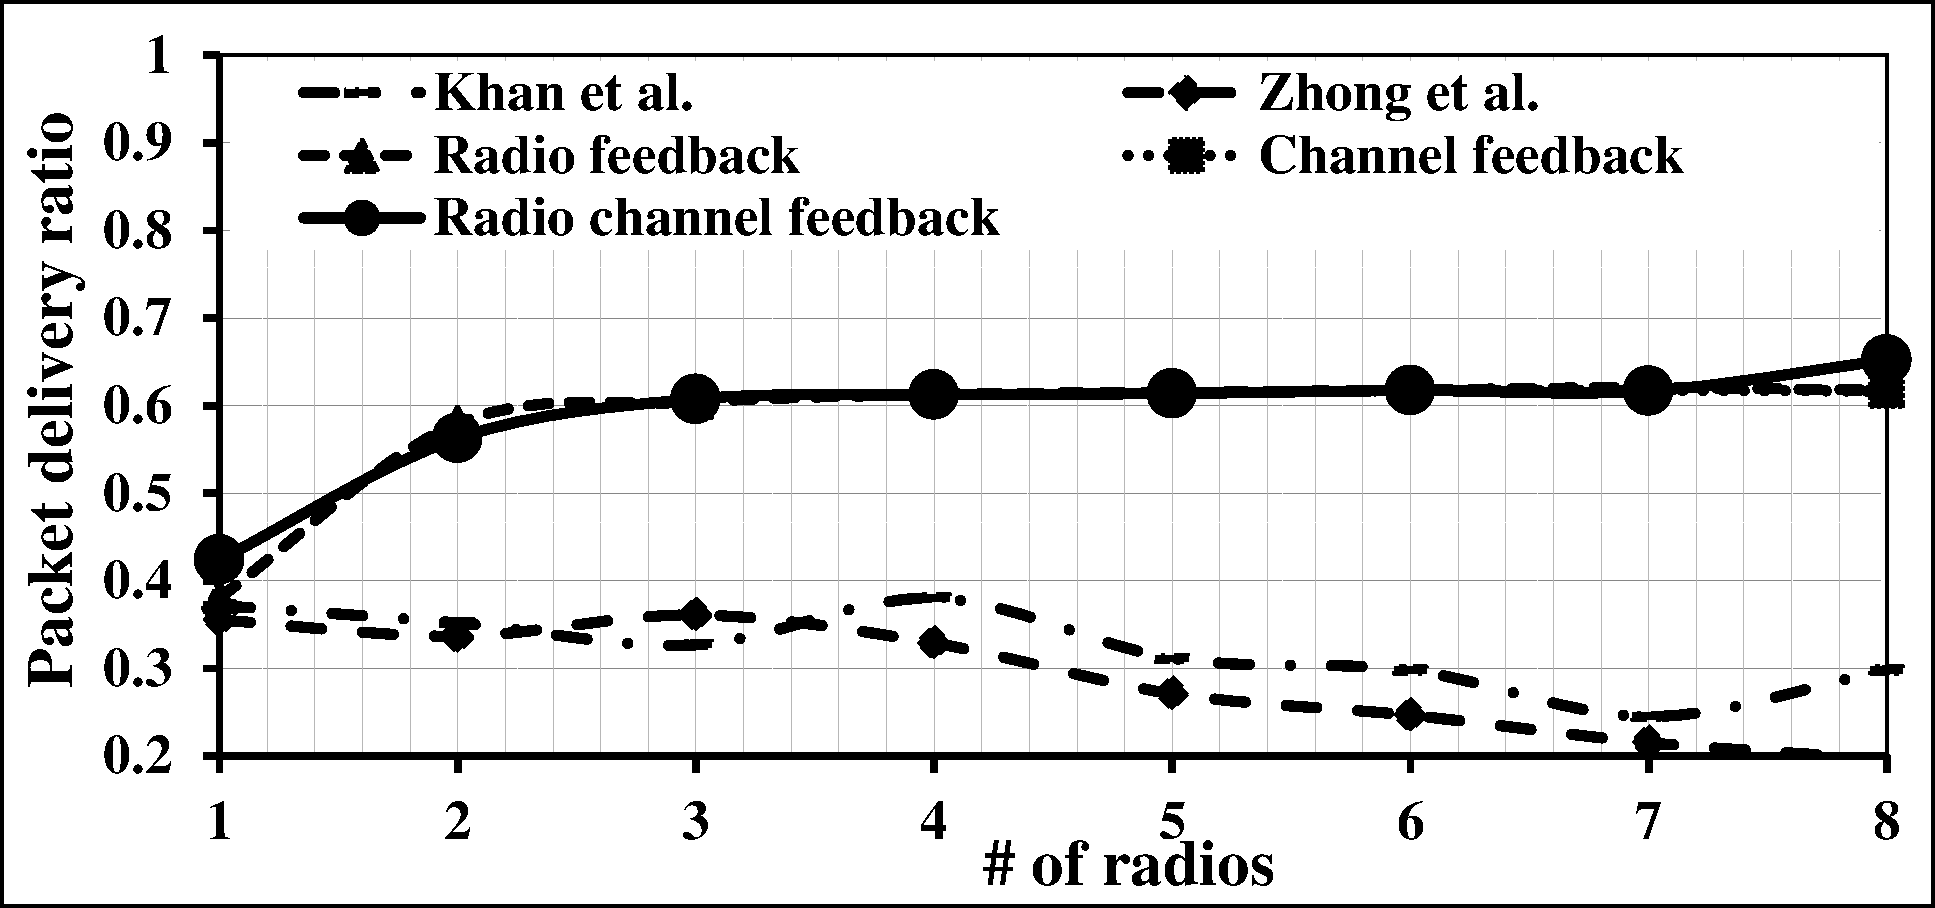
\includegraphics[width=\textwidth]{topology4/DeliveryRatio24d8}
        \caption{8Mbps application data rate}
        \label{fig:topology4PD4}
    \end{subfigure}
    ~\\
    \begin{subfigure}[t]{0.45\textwidth}
        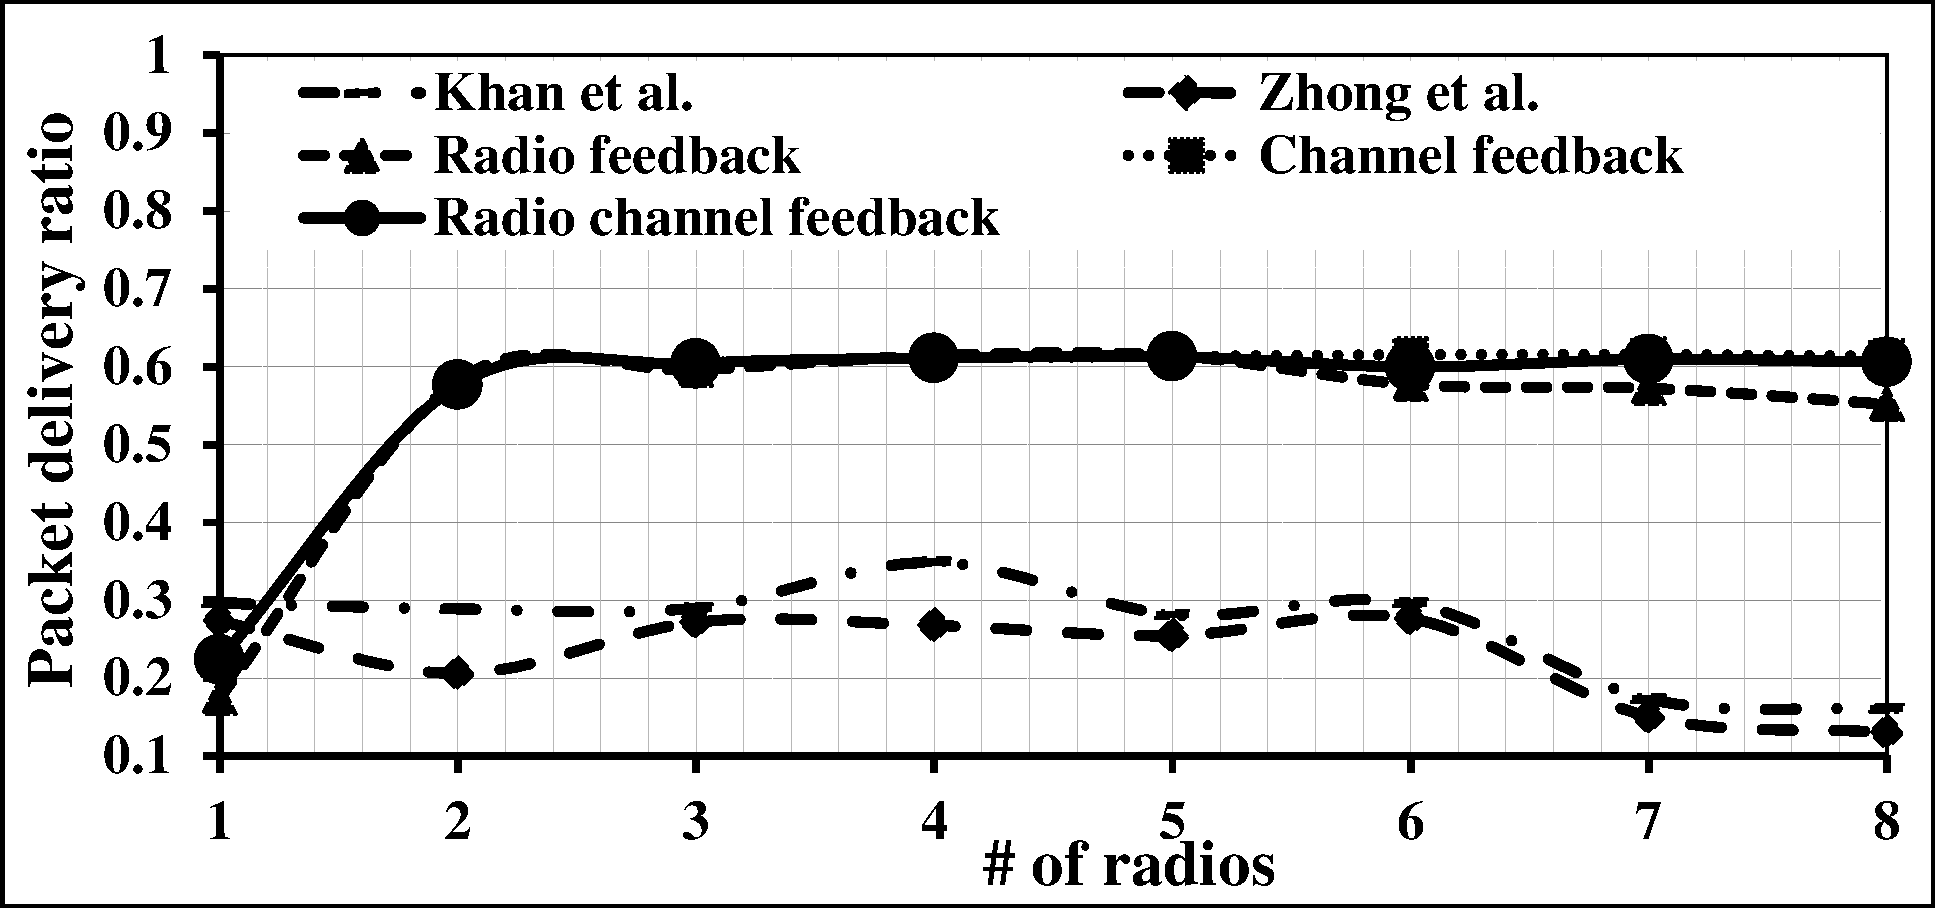
\includegraphics[width=\textwidth]{topology4/DeliveryRatio24d16}
        \caption{16Mbps application data rate}
        \label{fig:topology4PD5}
    \end{subfigure}
    ~
    \begin{subfigure}[t]{0.45\textwidth}
        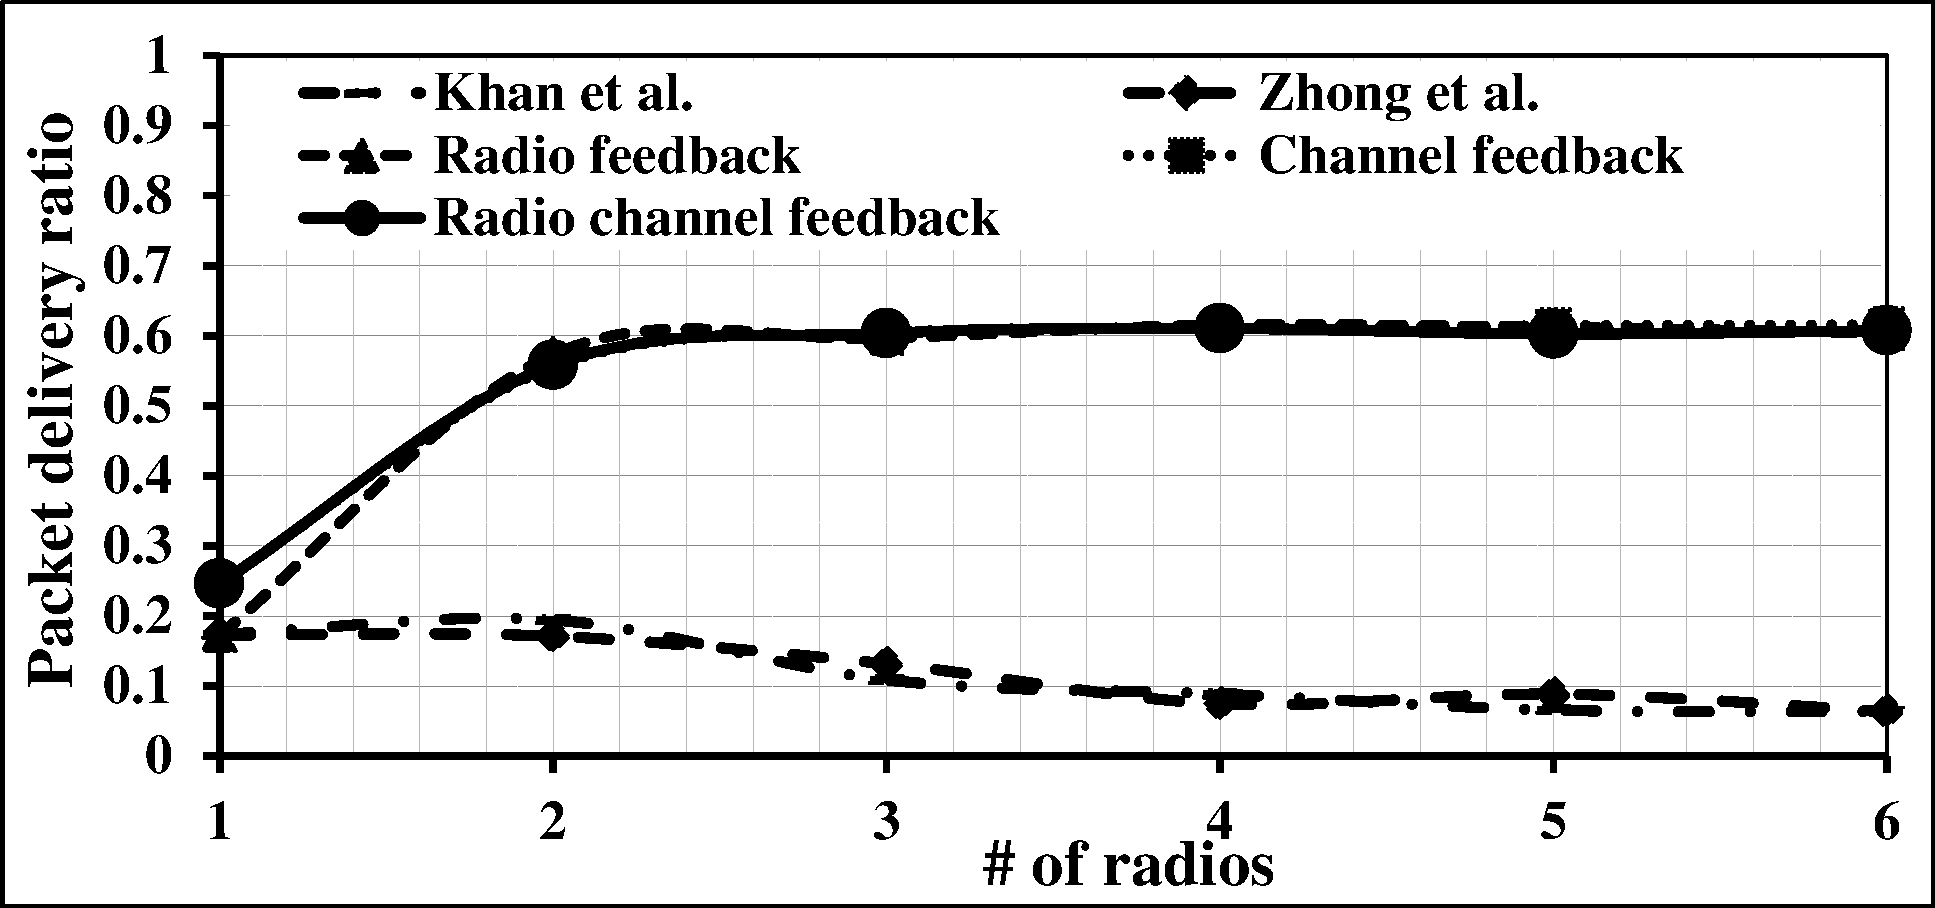
\includegraphics[width=\textwidth]{topology4/DeliveryRatio24d32}
        \caption{32Mbps application data rate}
        \label{fig:topology4PD6}
    \end{subfigure}
    \caption{Application layer packet delivery ratio with varying number of radios for various application data rates}
    \label{fig:topology4PD}
\end{figure*}


Fig.~\ref{fig:topology4P} compares the average packet drop ratio of our proposed approaches against that of the existing approaches.  As illustrated in \cref{fig:topology4P}, the feedback-based approach achieves significantly lower packet drop ratios than all the existing ones. The feedback-based approach is also able to reduce the packet drop ratio significantly at lower data rates (1-8 Mbps) with the exploitation of multiple radios. However, at higher application data rates (16 and 32 Mbps), most of the packets get dropped resulting in high drop ratios. This explains why the network throughput at higher data rate does not improve even after the introduction of multiple data transmission radios.

Fig.~\ref{fig:topology4PD} shows the application layer packet delivery ratio of our proposed approaches against that of the existing approaches. Due to the efficient exploitation of multiple radios, our proposed approaches obtain significantly better packet delivery ratio than that achieved with the existing appraoches.

Table~\ref{tab:topology4RadioImprovement}, \ref{tab:topology4ChannelImprovement}, and \ref{tab:topology4RadioChannelImprovement} summarize average performance improvement using feedback-based approaches in comparison to the approaches proposed by Khan et al.,~\cite{khan2015towards} and Zhong et al.~\cite{zhong2014capacity}. The tables shows that the proposed approach outperforms the existing approaches in terms of all the performance metrics except end-to-end delay. In terms of total network throughput, the proposed approach obtains an average of 51\% improvement over the two existing approaches. Moreover, the proposed approach decreases packet drop ratio on an average 35\% and increases application layer packet delivery ratio on an average 32\% compared to existing approaches. Even though, the feedback-based approach experiences the higher delay in some cases, in average, the delay is improved by 13\% on an average.
%\begin{figure*}[!htbp]
    \centering
    \begin{subfigure}[t]{0.45\textwidth}
        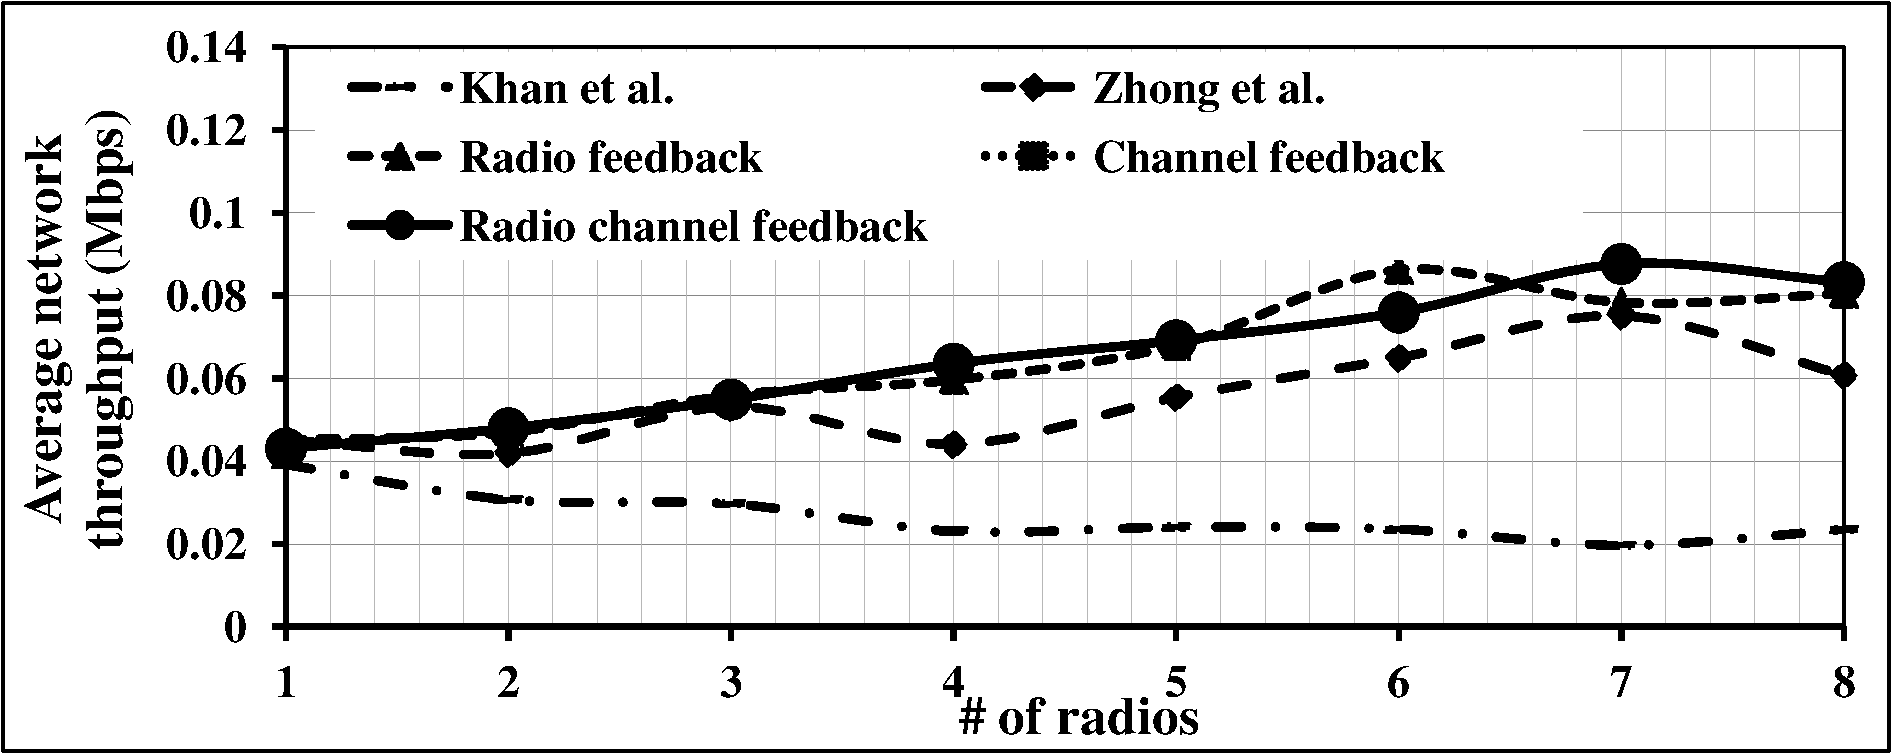
\includegraphics[width=\textwidth]{topology4/Throughput24d1}
        \caption{1Mbps application data rate}
        \label{fig:topology4T1}
    \end{subfigure}
    ~
    \begin{subfigure}[t]{0.45\textwidth}
        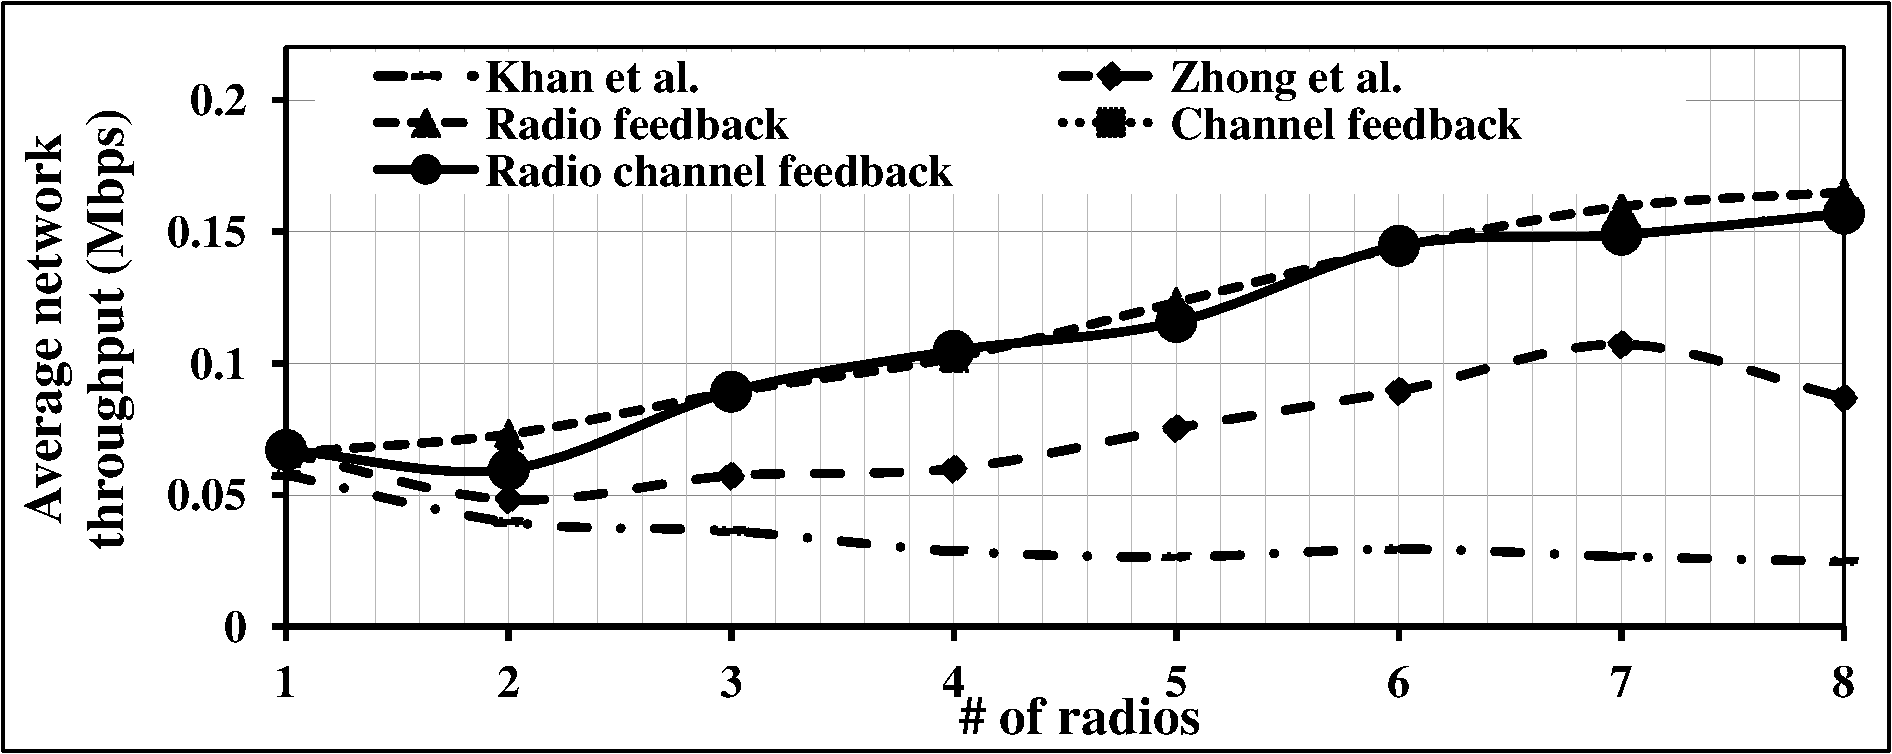
\includegraphics[width=\textwidth]{topology4/Throughput24d2}
        \caption{2Mbps application data rate}
        \label{fig:topology4T2}
    \end{subfigure}
    ~\\
    \begin{subfigure}[t]{0.45\textwidth}
        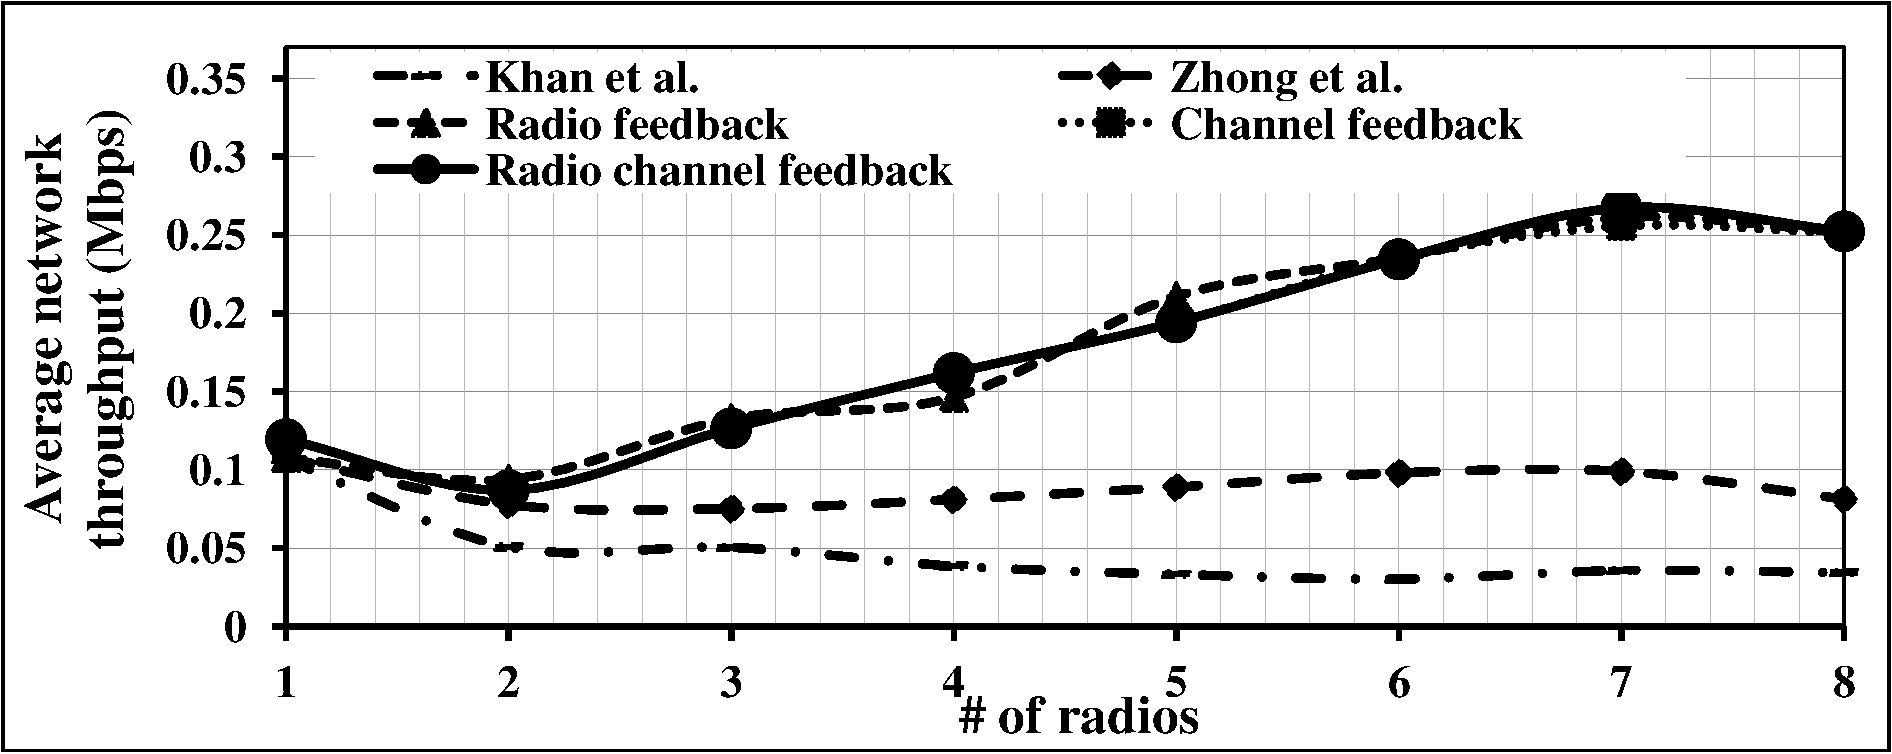
\includegraphics[width=\textwidth]{topology4/Throughput24d4}
        \caption{4Mbps application data rate}
        \label{fig:topology4T3}
    \end{subfigure}
    ~
    \begin{subfigure}[t]{0.45\textwidth}
        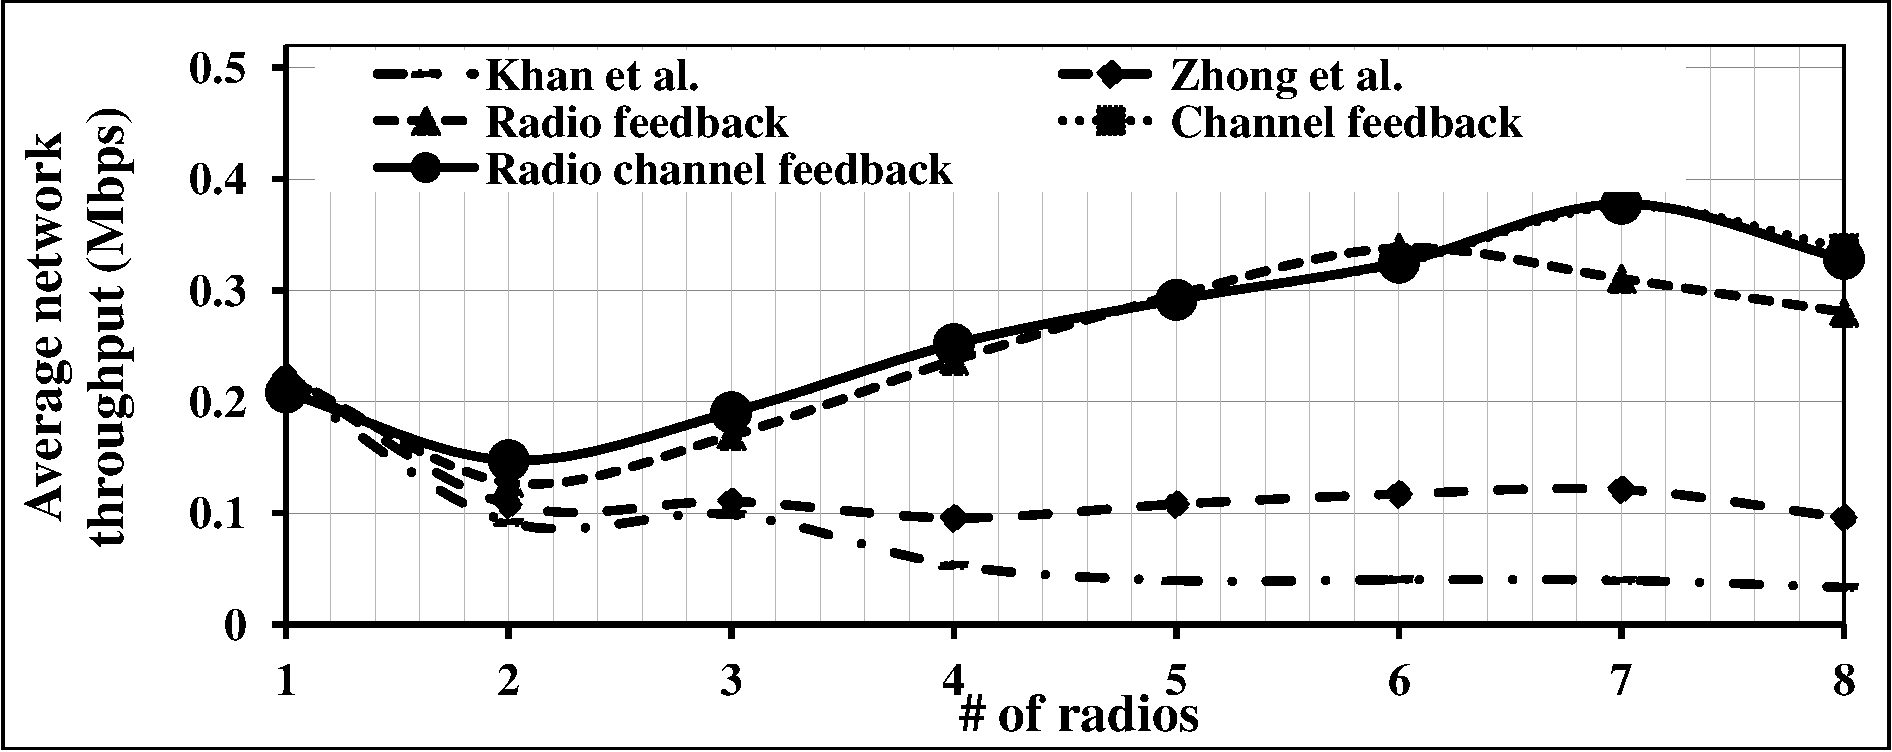
\includegraphics[width=\textwidth]{topology4/Throughput24d8}
        \caption{8Mbps application data rate}
        \label{fig:topology4T4}
    \end{subfigure}
    ~\\
    \begin{subfigure}[t]{0.45\textwidth}
        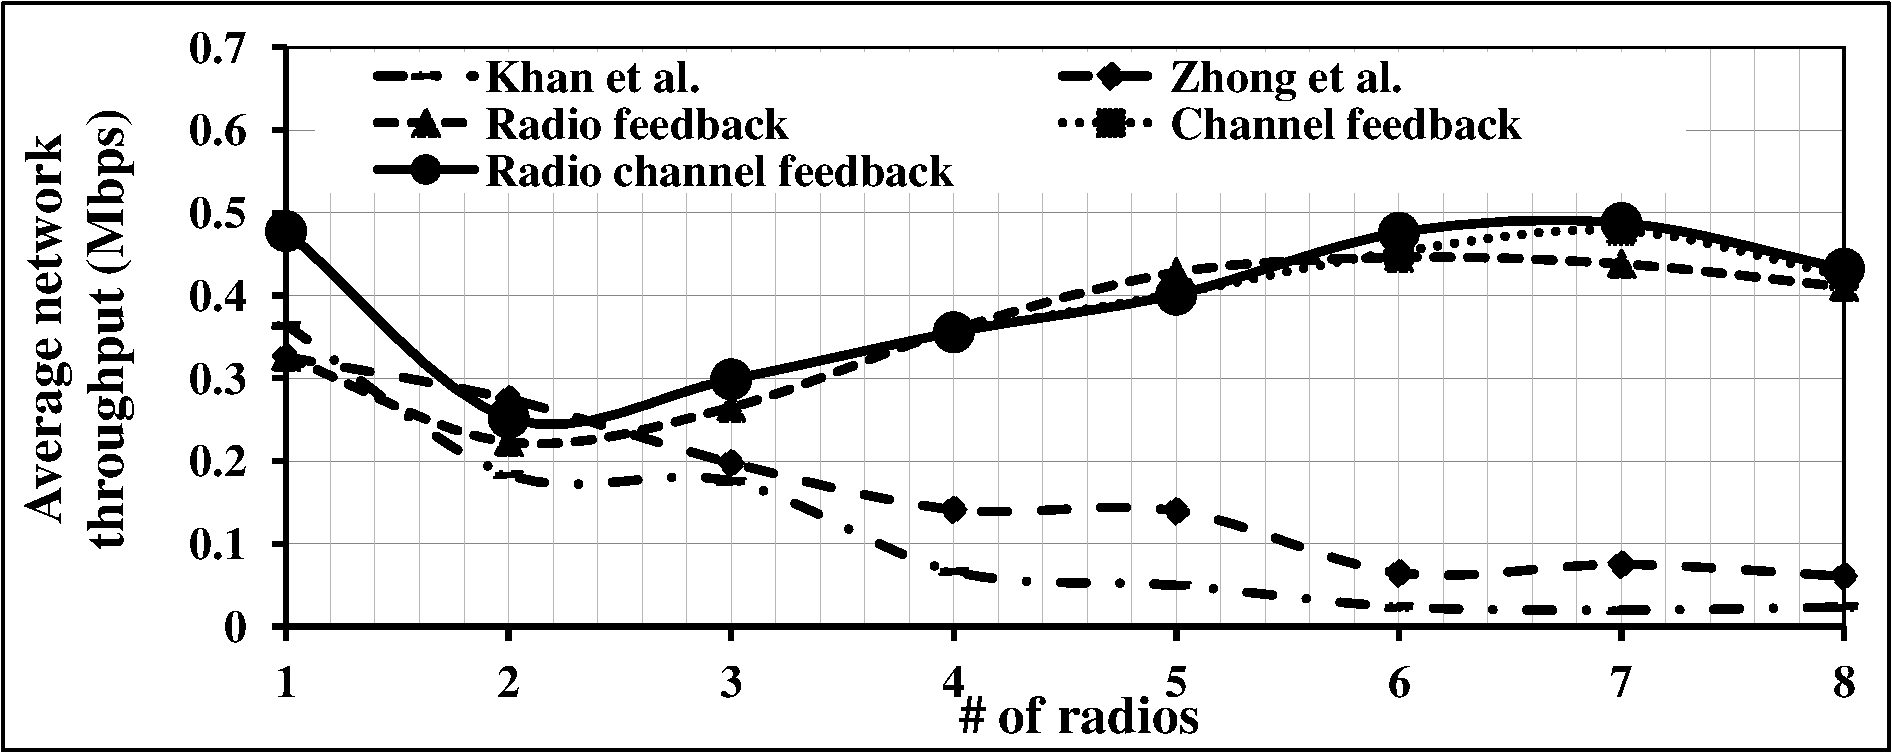
\includegraphics[width=\textwidth]{topology4/Throughput24d16}
        \caption{16Mbps application data rate}
        \label{fig:topology4T5}
    \end{subfigure}
    ~
    \begin{subfigure}[t]{0.45\textwidth}
        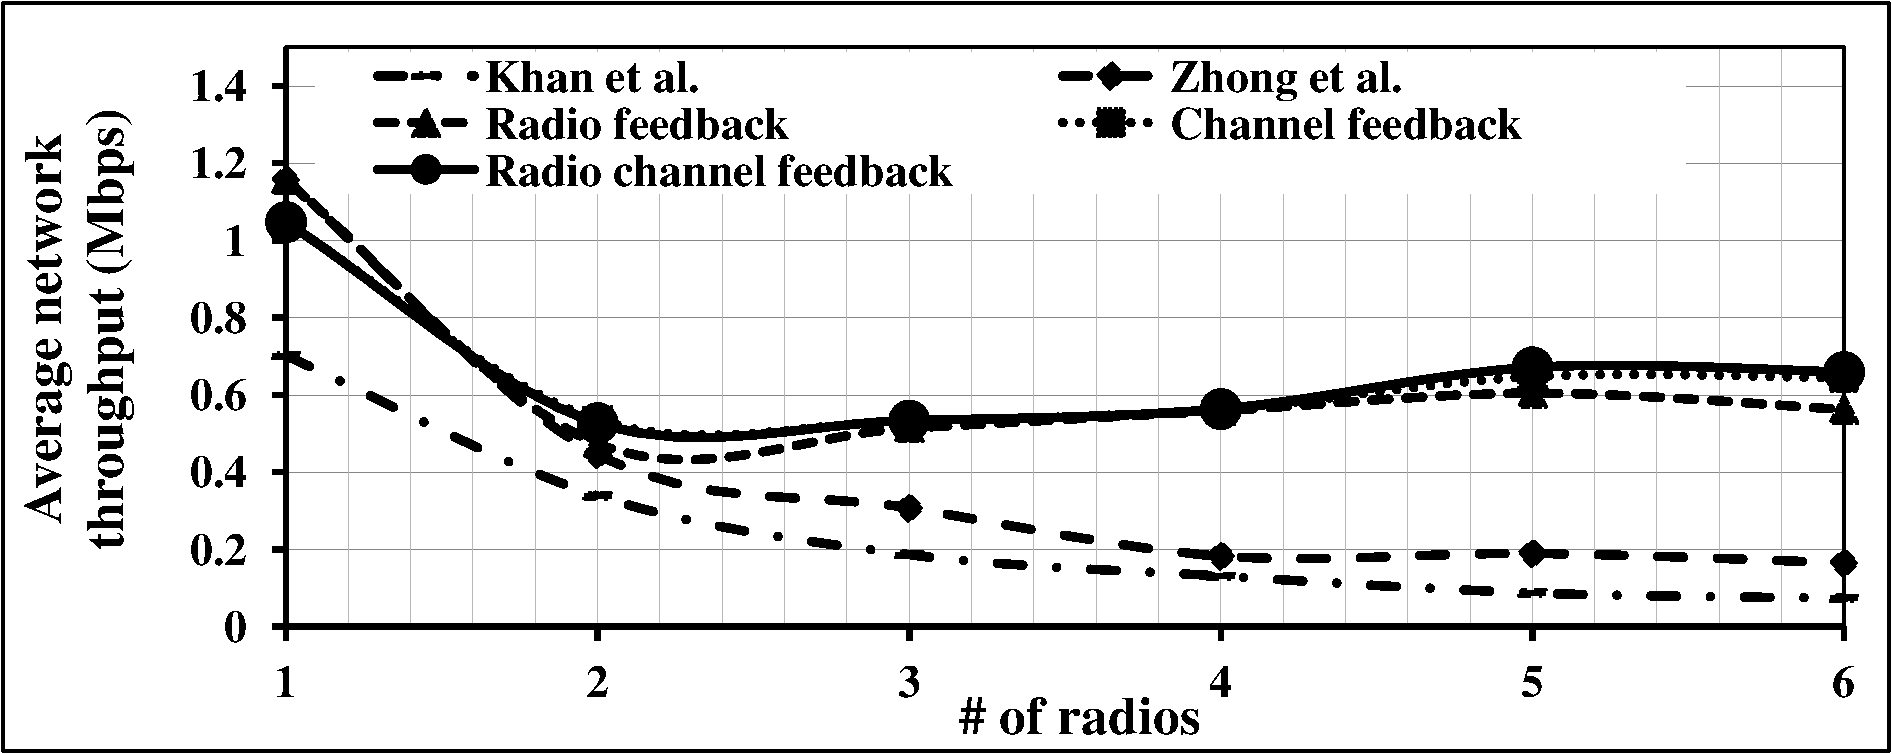
\includegraphics[width=\textwidth]{topology4/Throughput24d32}
        \caption{32Mbps application data rate}
        \label{fig:topology4T6}
    \end{subfigure}
    \caption{Average network throughput with varying number of radios for various application data rates}
    \label{fig:topology4T}
\end{figure*}

\begin{figure*}[!htbp]
    \centering
    \begin{subfigure}[t]{0.45\textwidth}
        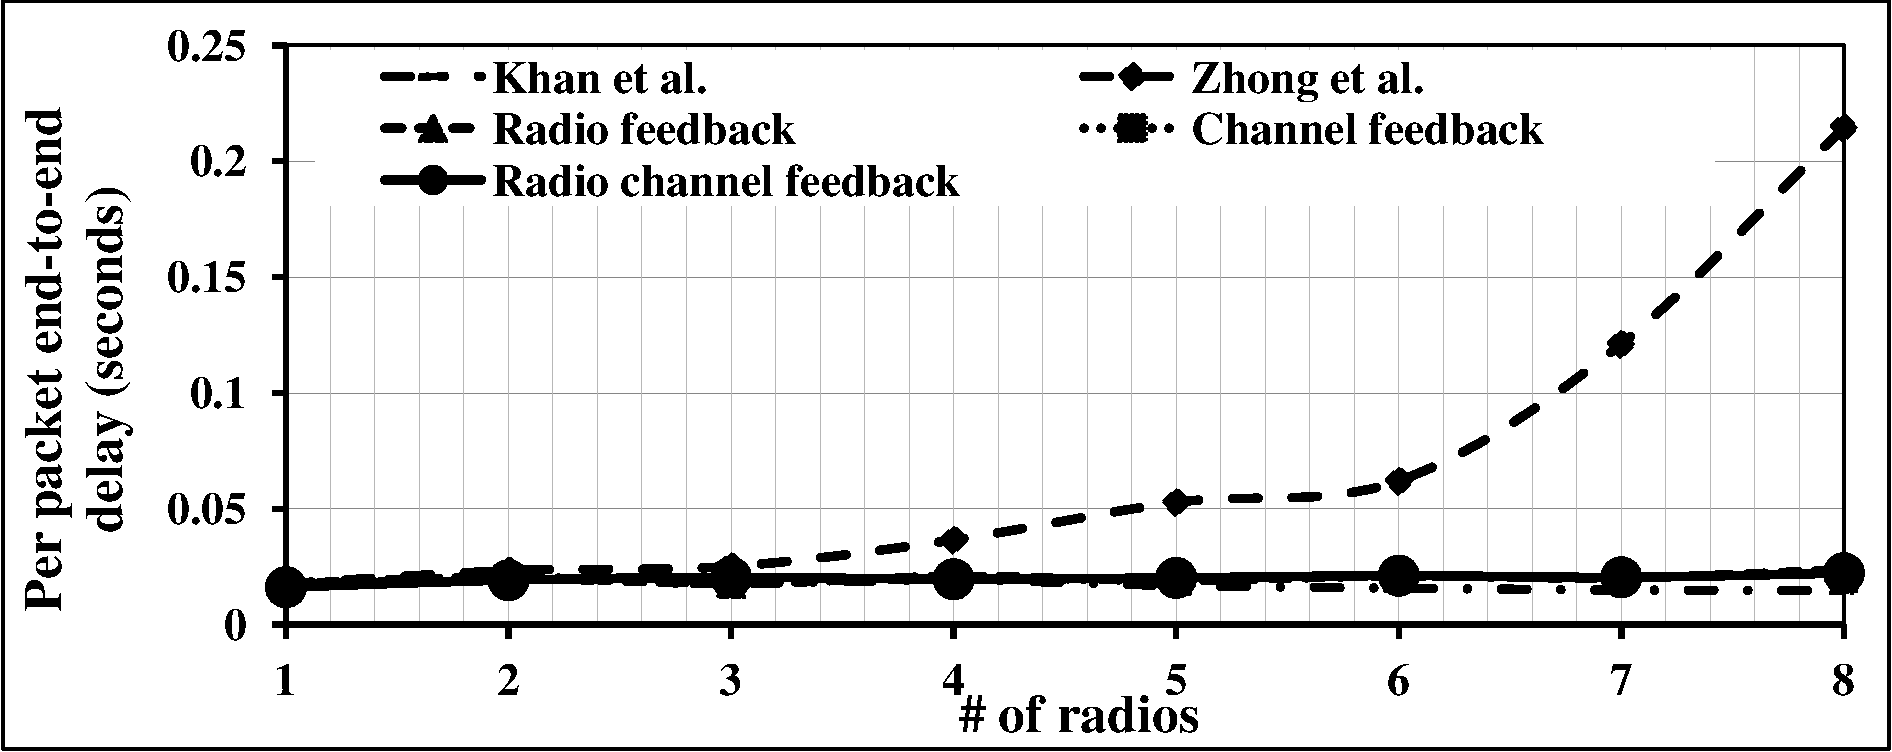
\includegraphics[width=\textwidth]{topology4/Delay24d1}
        \caption{1Mbps application data rate}
        \label{fig:topology4D1}
    \end{subfigure}
    ~
    \begin{subfigure}[t]{0.45\textwidth}
        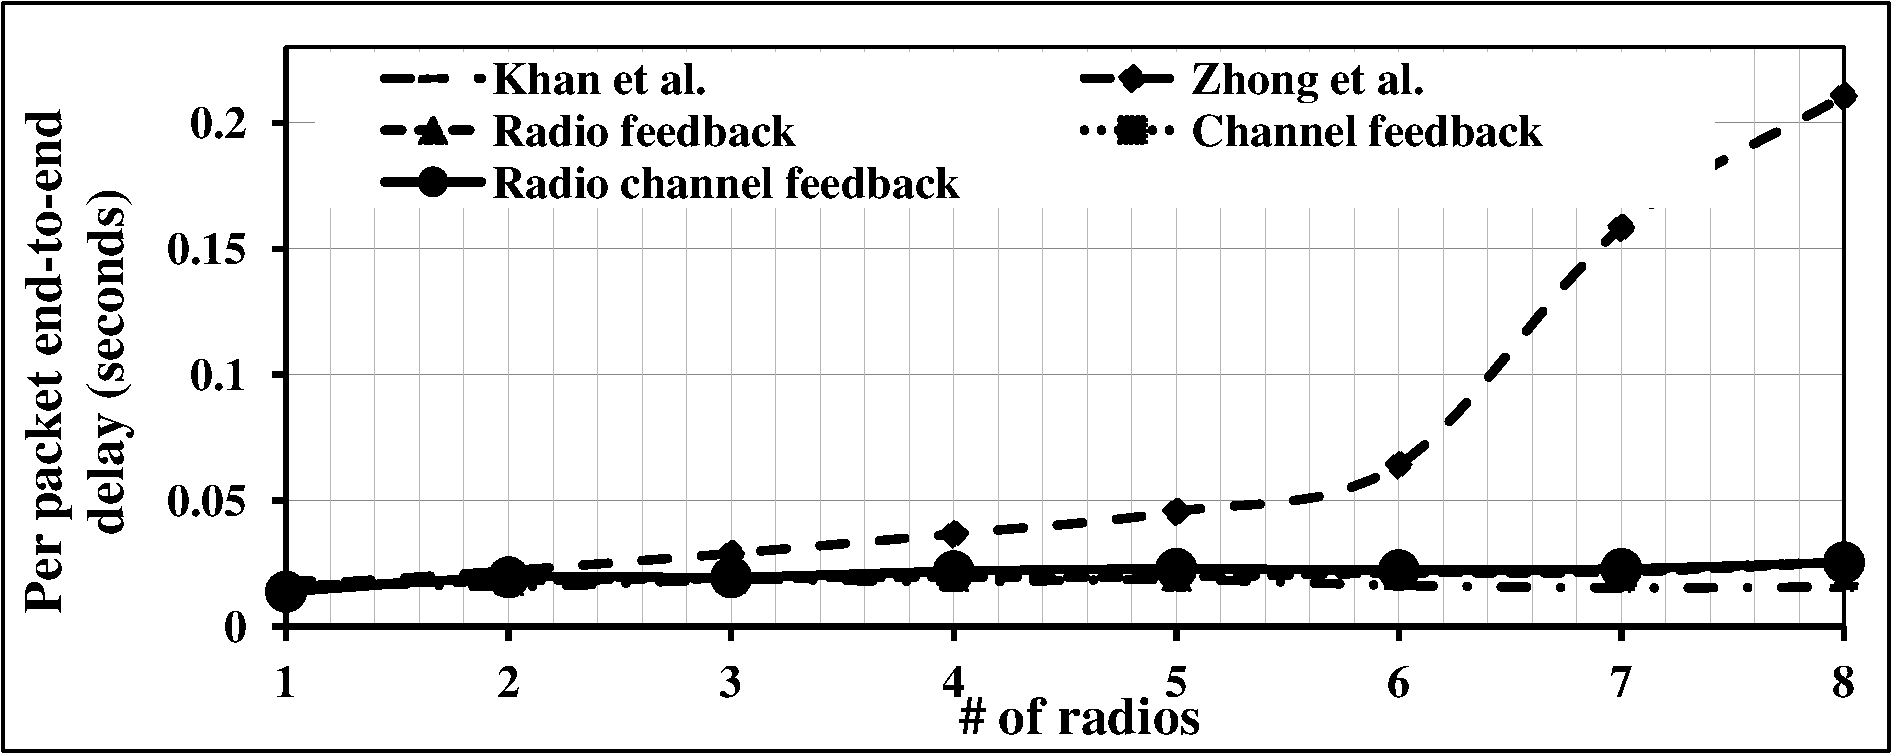
\includegraphics[width=\textwidth]{topology4/Delay24d2}
        \caption{2Mbps application data rate}
        \label{fig:topology4D2}
    \end{subfigure}
    ~\\
    \begin{subfigure}[t]{0.45\textwidth}
        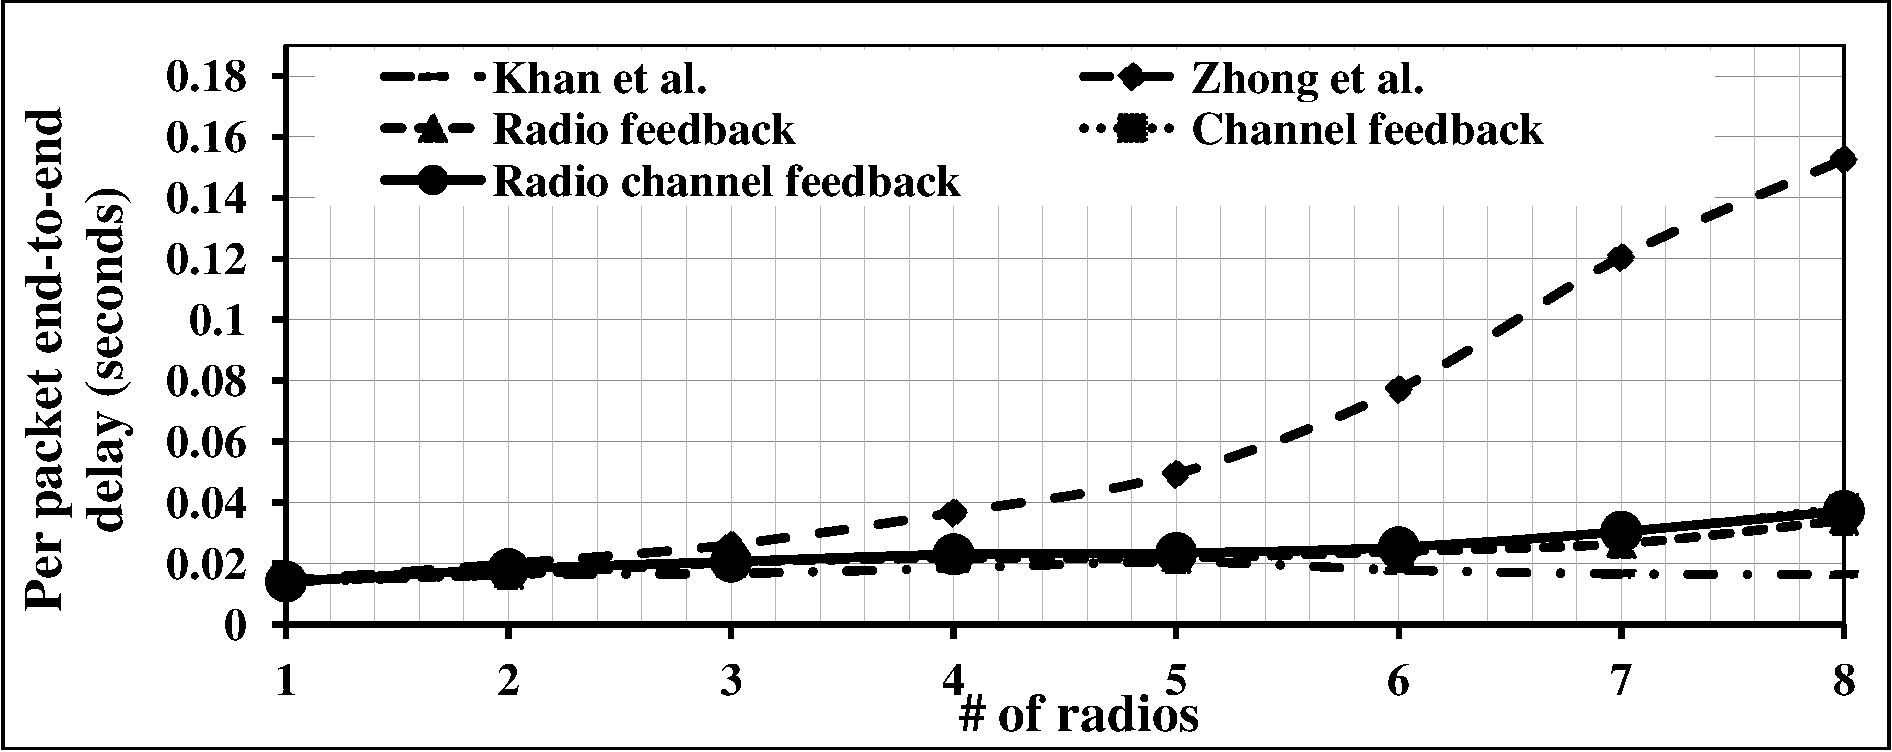
\includegraphics[width=\textwidth]{topology4/Delay24d4}
        \caption{4Mbps application data rate}
        \label{fig:topology4D3}
    \end{subfigure}
    ~
    \begin{subfigure}[t]{0.45\textwidth}
        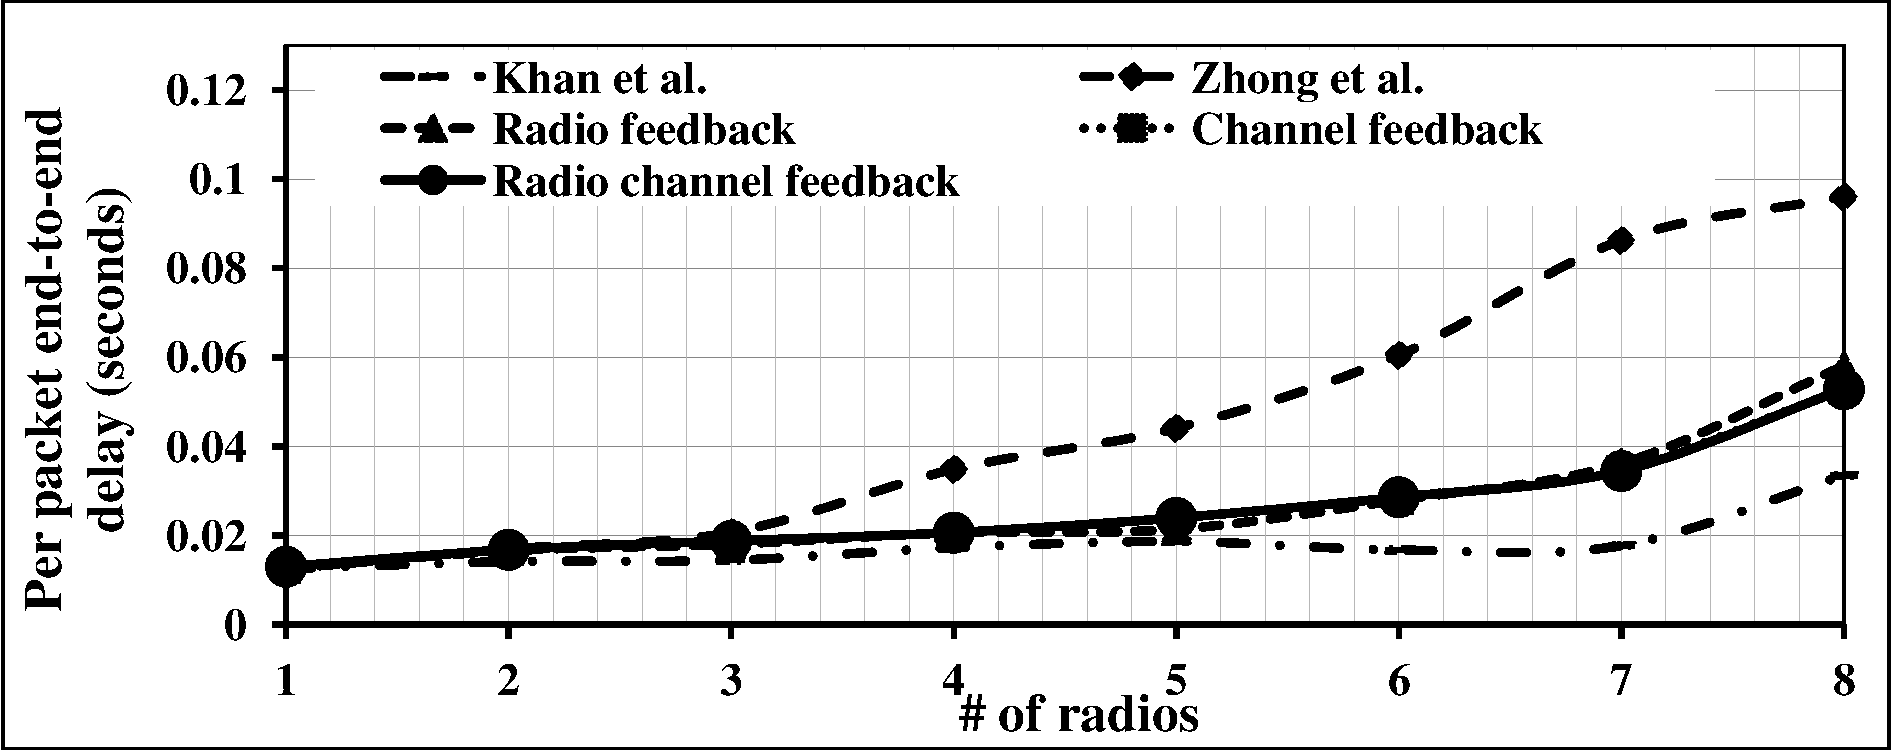
\includegraphics[width=\textwidth]{topology4/Delay24d8}
        \caption{8Mbps application data rate}
        \label{fig:topology4D4}
    \end{subfigure}
    ~\\
    \begin{subfigure}[t]{0.45\textwidth}
        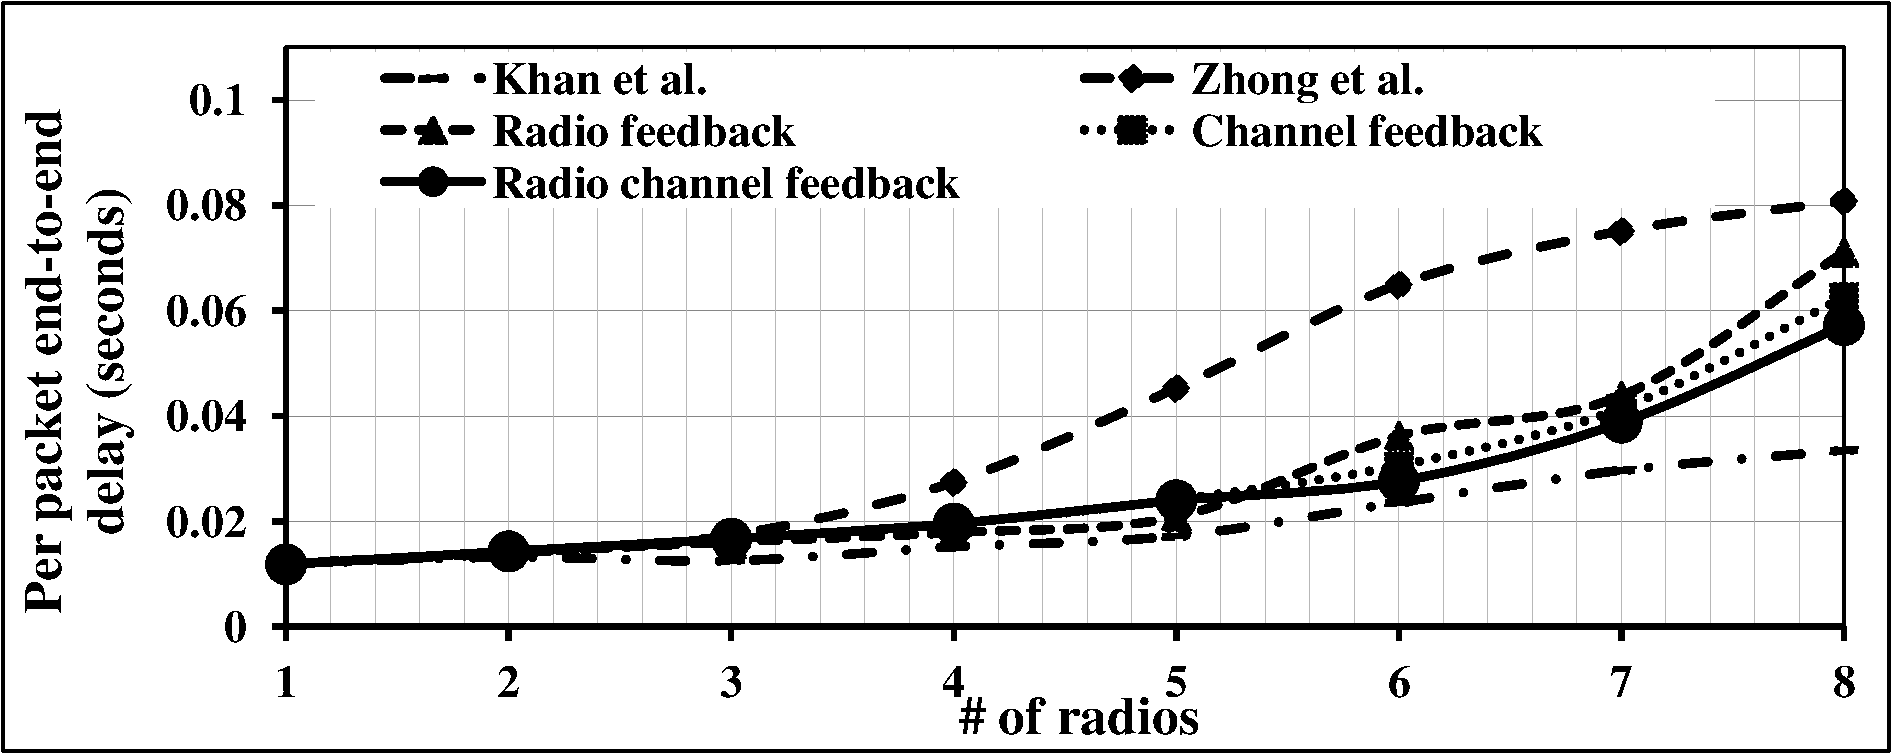
\includegraphics[width=\textwidth]{topology4/Delay24d16}
        \caption{16Mbps application data rate}
        \label{fig:topology4D5}
    \end{subfigure}
    ~
    \begin{subfigure}[t]{0.45\textwidth}
        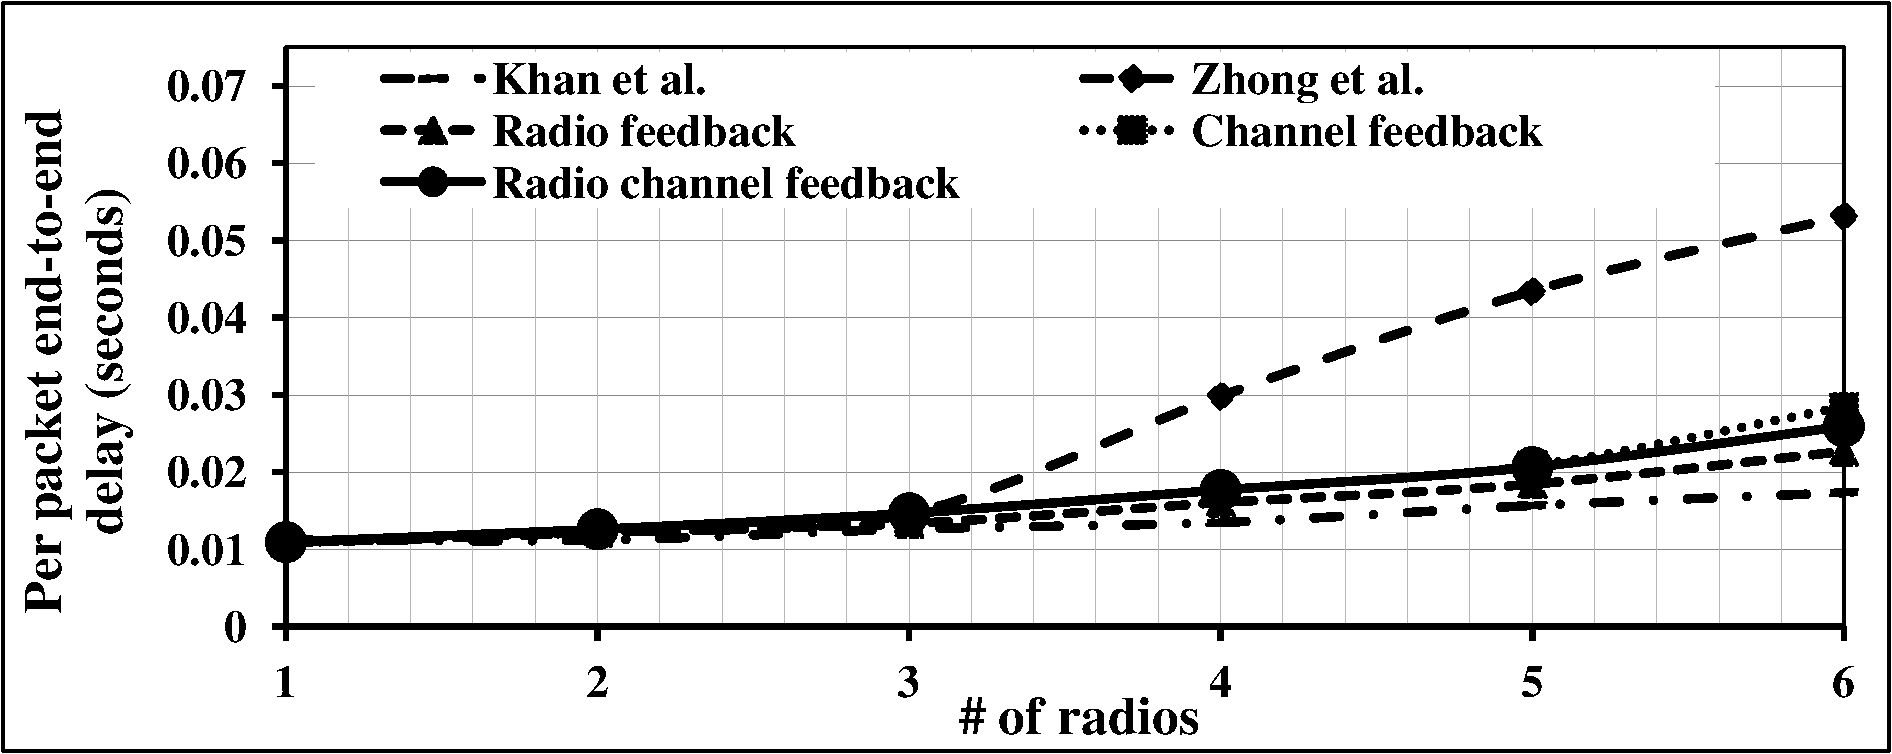
\includegraphics[width=\textwidth]{topology4/Delay24d32}
        \caption{32Mbps application data rate}
        \label{fig:topology4D6}
    \end{subfigure}
    \caption{Average end-to-end delay with varying number of radios for various application data rates}
    \label{fig:topology4D}
\end{figure*}

\begin{landscape}
\begin{figure*}[!htbp]
    \centering
    \begin{subfigure}[t]{0.625\textwidth}
        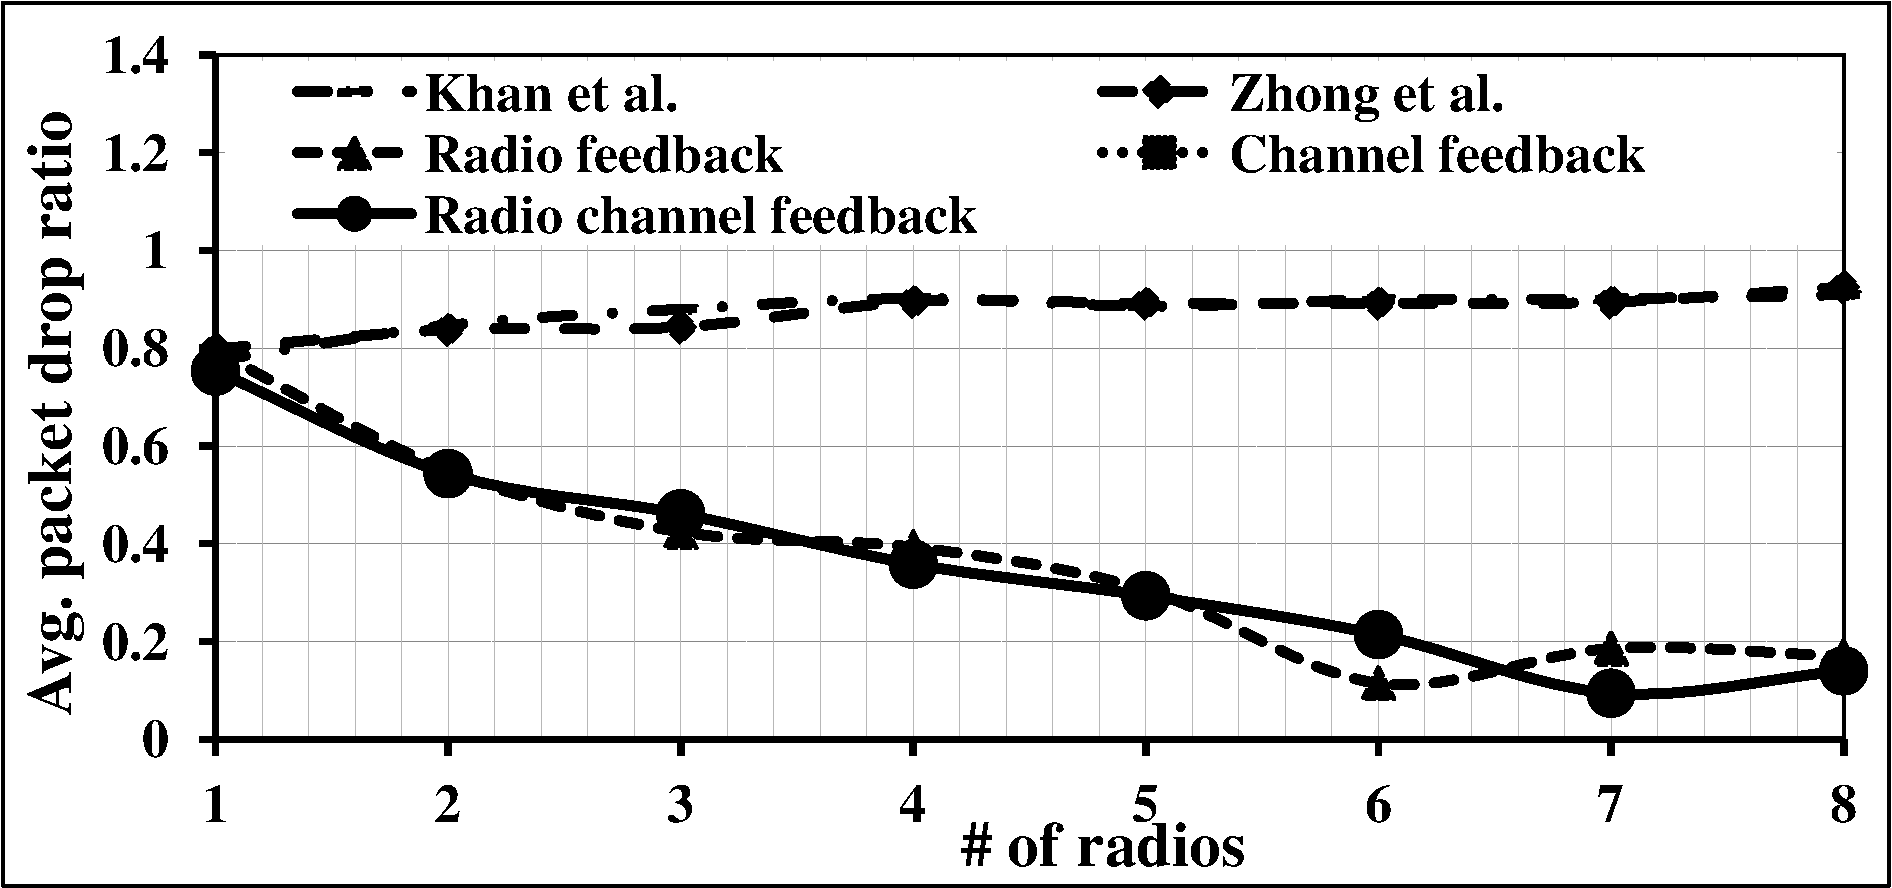
\includegraphics[width=\textwidth]{topology4/PacketDropRatio24d1}
        \caption{1Mbps application data rate}
        \label{fig:topology4P1}
    \end{subfigure}
    ~
    \begin{subfigure}[t]{0.625\textwidth}
        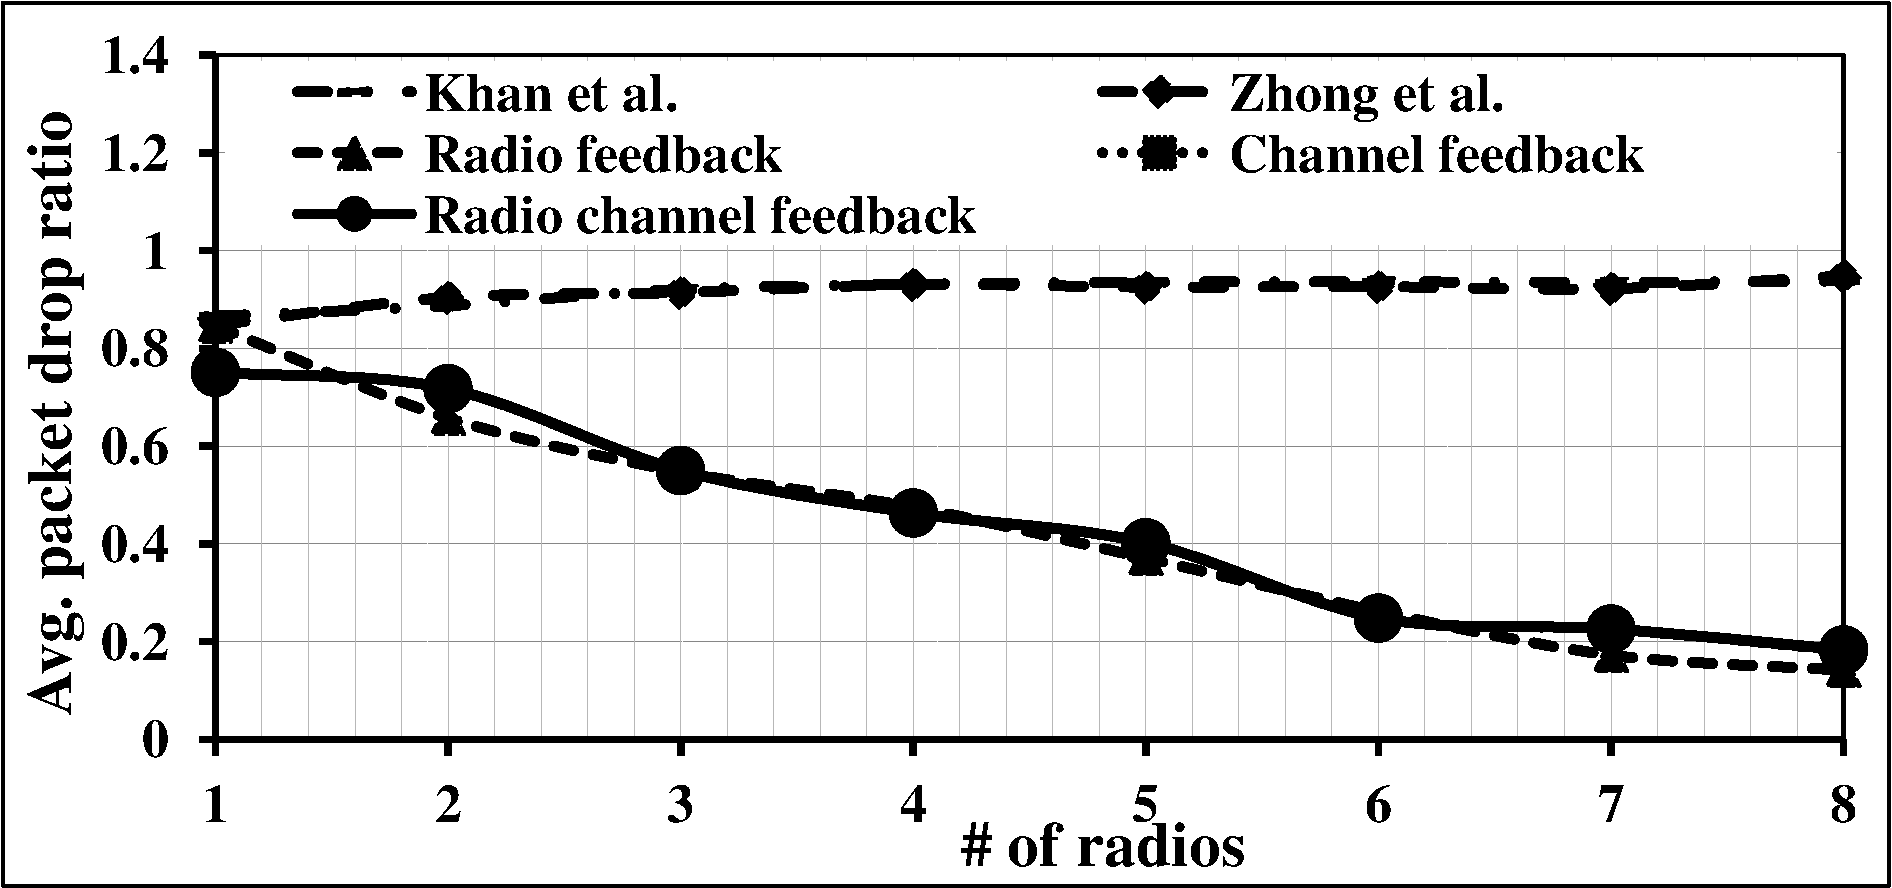
\includegraphics[width=\textwidth]{topology4/PacketDropRatio24d2}
        \caption{2Mbps application data rate}
        \label{fig:topology4P2}
    \end{subfigure}
    ~\\
    \begin{subfigure}[t]{0.625\textwidth}
        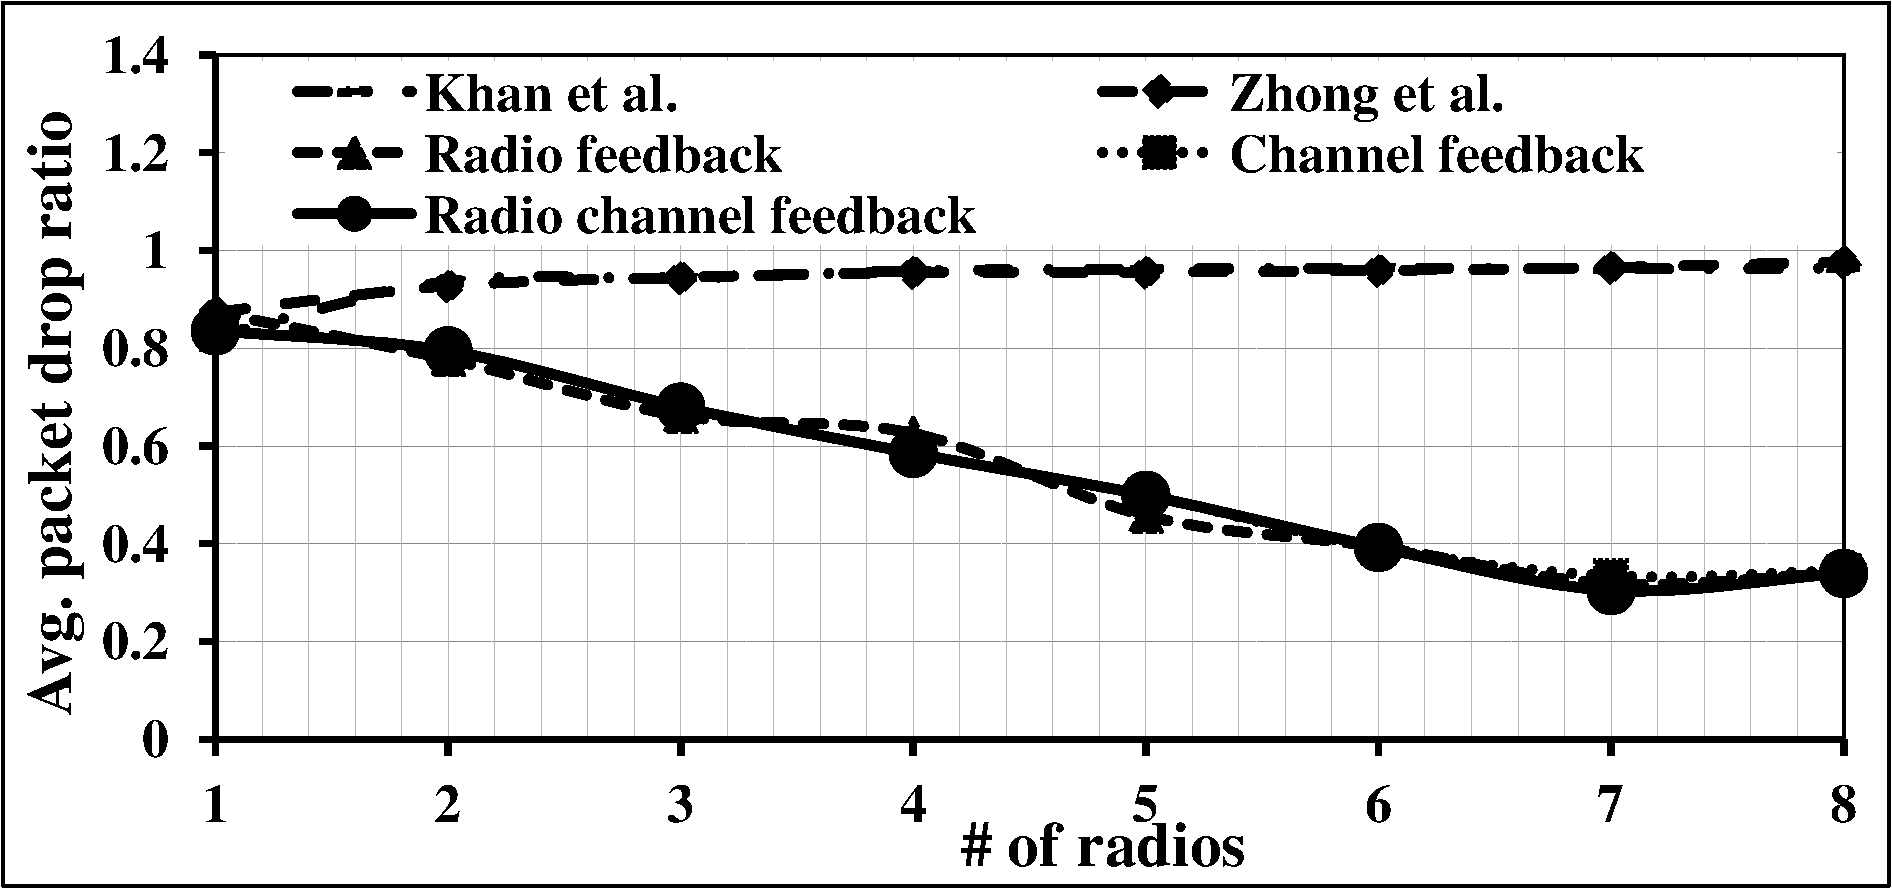
\includegraphics[width=\textwidth]{topology4/PacketDropRatio24d4}
        \caption{4Mbps application data rate}
        \label{fig:topology4P3}
    \end{subfigure}
    ~
    \begin{subfigure}[t]{0.625\textwidth}
        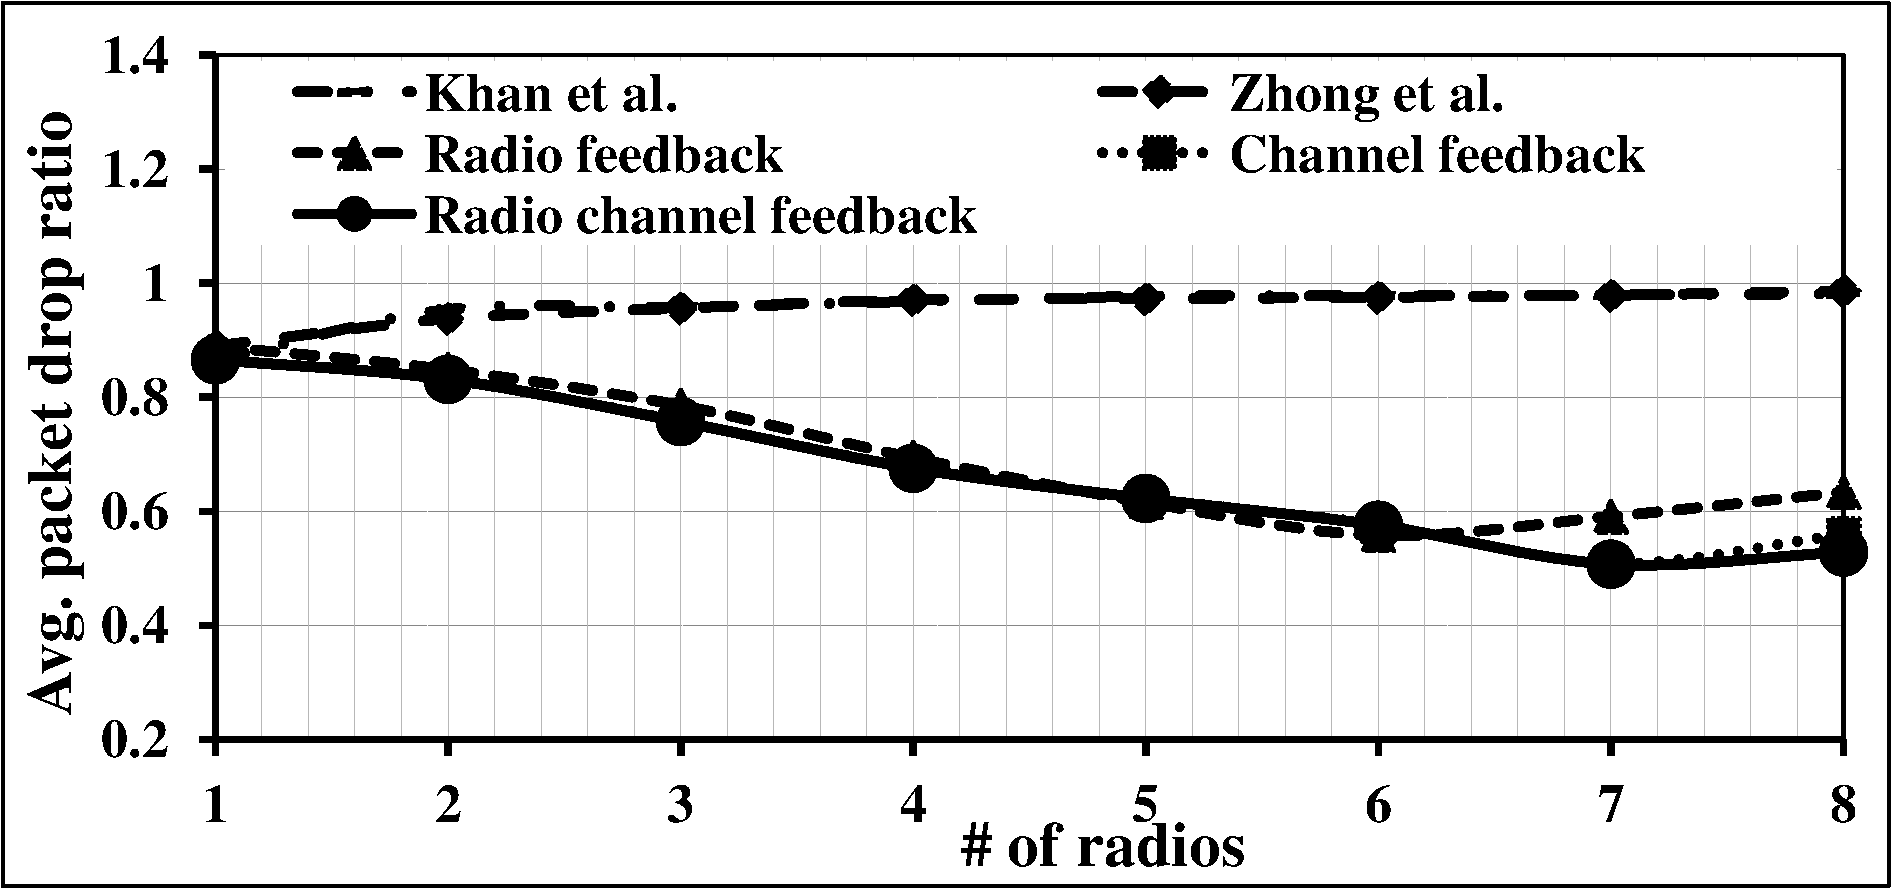
\includegraphics[width=\textwidth]{topology4/PacketDropRatio24d8}
        \caption{8Mbps application data rate}
        \label{fig:topology4P4}
    \end{subfigure}
    ~\\
    \begin{subfigure}[t]{0.625\textwidth}
        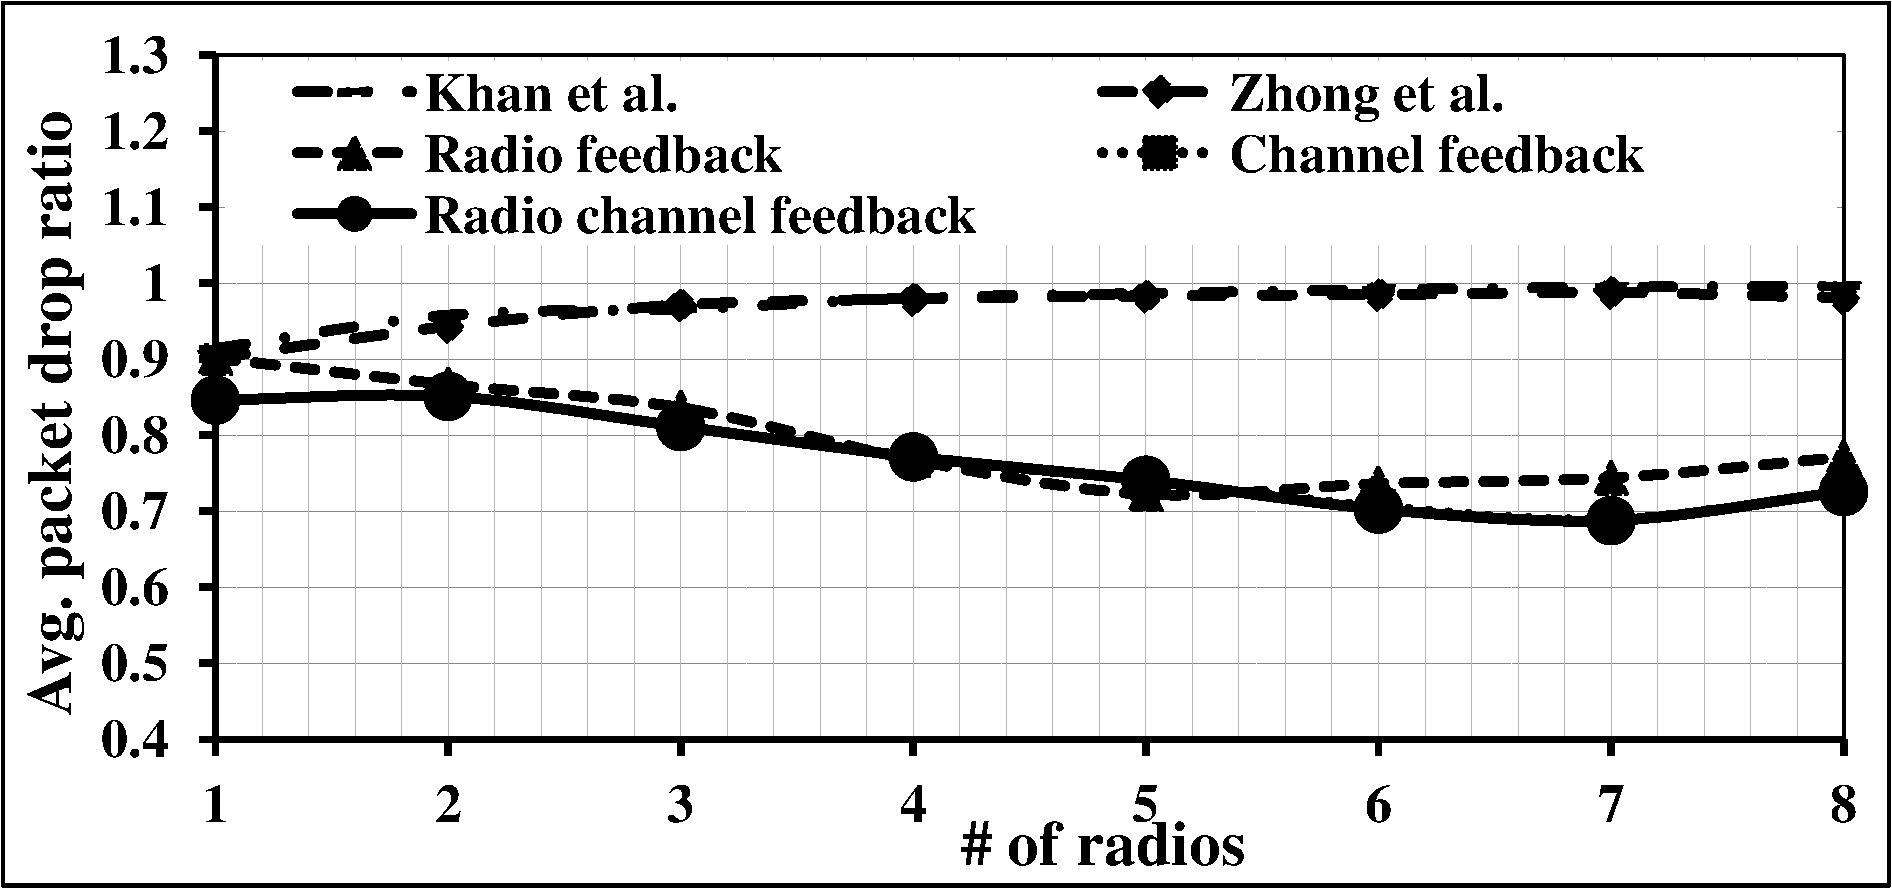
\includegraphics[width=\textwidth]{topology4/PacketDropRatio24d16}
        \caption{16Mbps application data rate}
        \label{fig:topology4P5}
    \end{subfigure}
    ~
    \begin{subfigure}[t]{0.625\textwidth}
        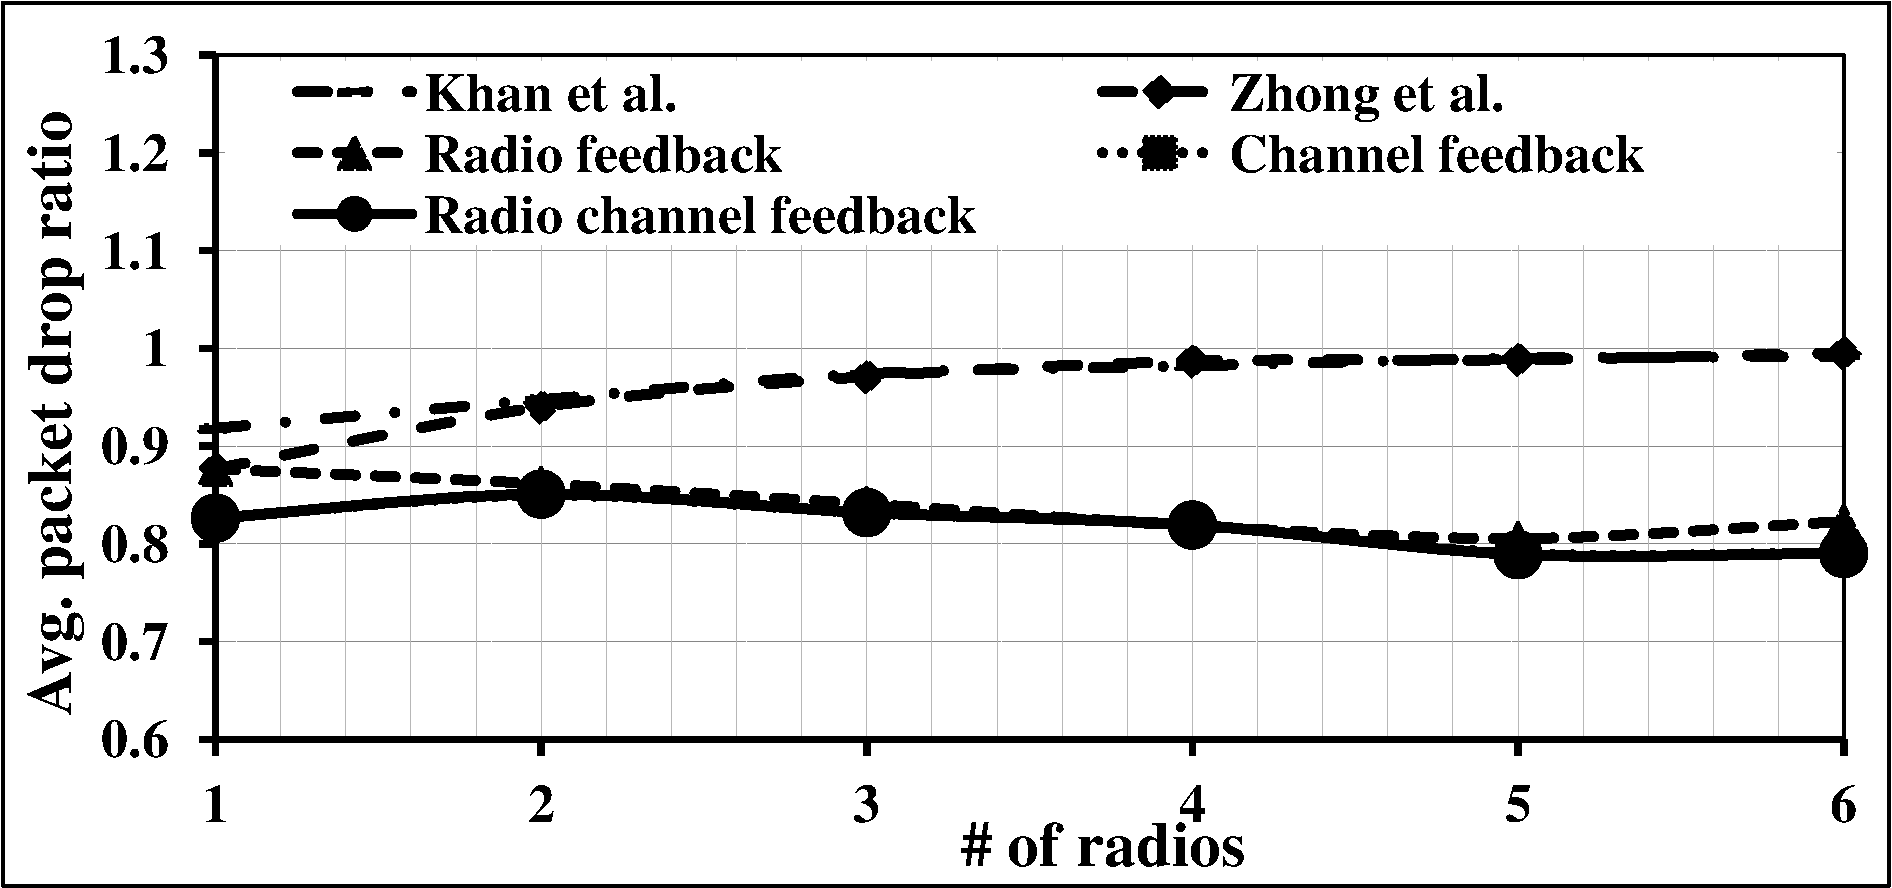
\includegraphics[width=\textwidth]{topology4/PacketDropRatio24d32}
        \caption{32Mbps application data rate}
        \label{fig:topology4P6}
    \end{subfigure}
    \caption{Average packet drop ratio with varying number of radios for various application data rates}
    \label{fig:topology4P}
\end{figure*}
\end{landscape}

\begin{figure*}[!htbp]
    \centering
    \begin{subfigure}[t]{0.45\textwidth}
        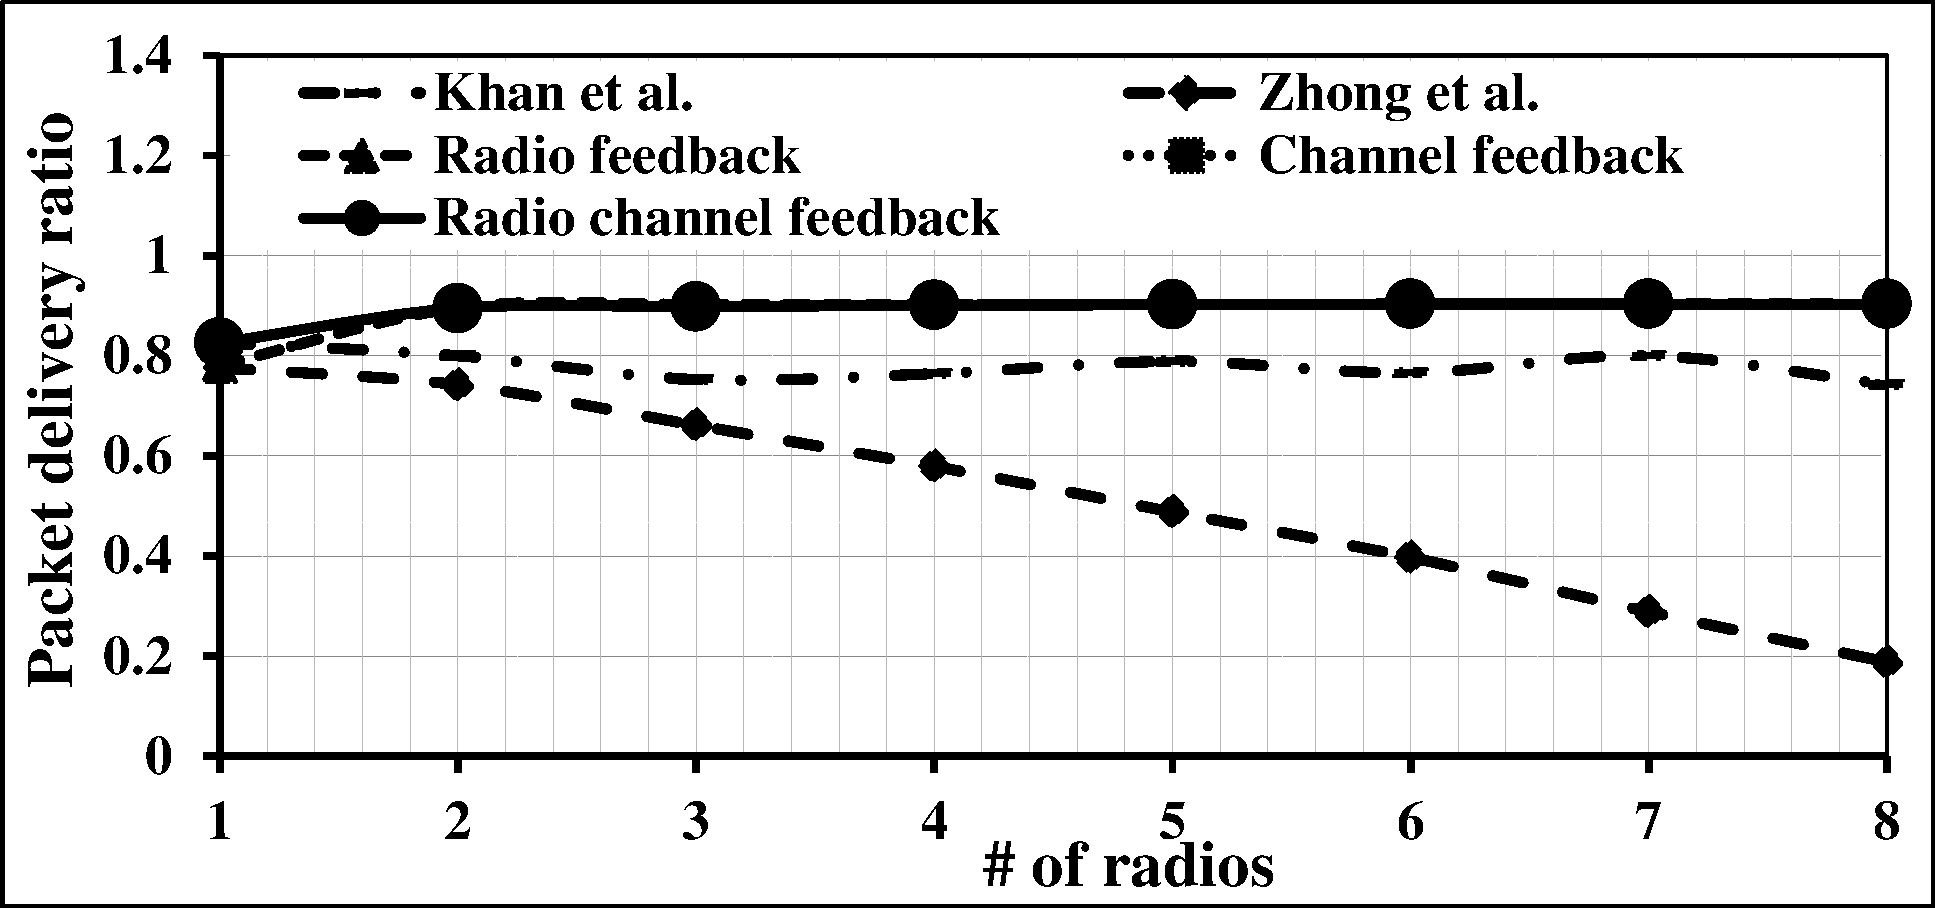
\includegraphics[width=\textwidth]{topology4/DeliveryRatio24d1}
        \caption{1Mbps application data rate}
        \label{fig:topology4PD1}
    \end{subfigure}
    ~
    \begin{subfigure}[t]{0.45\textwidth}
        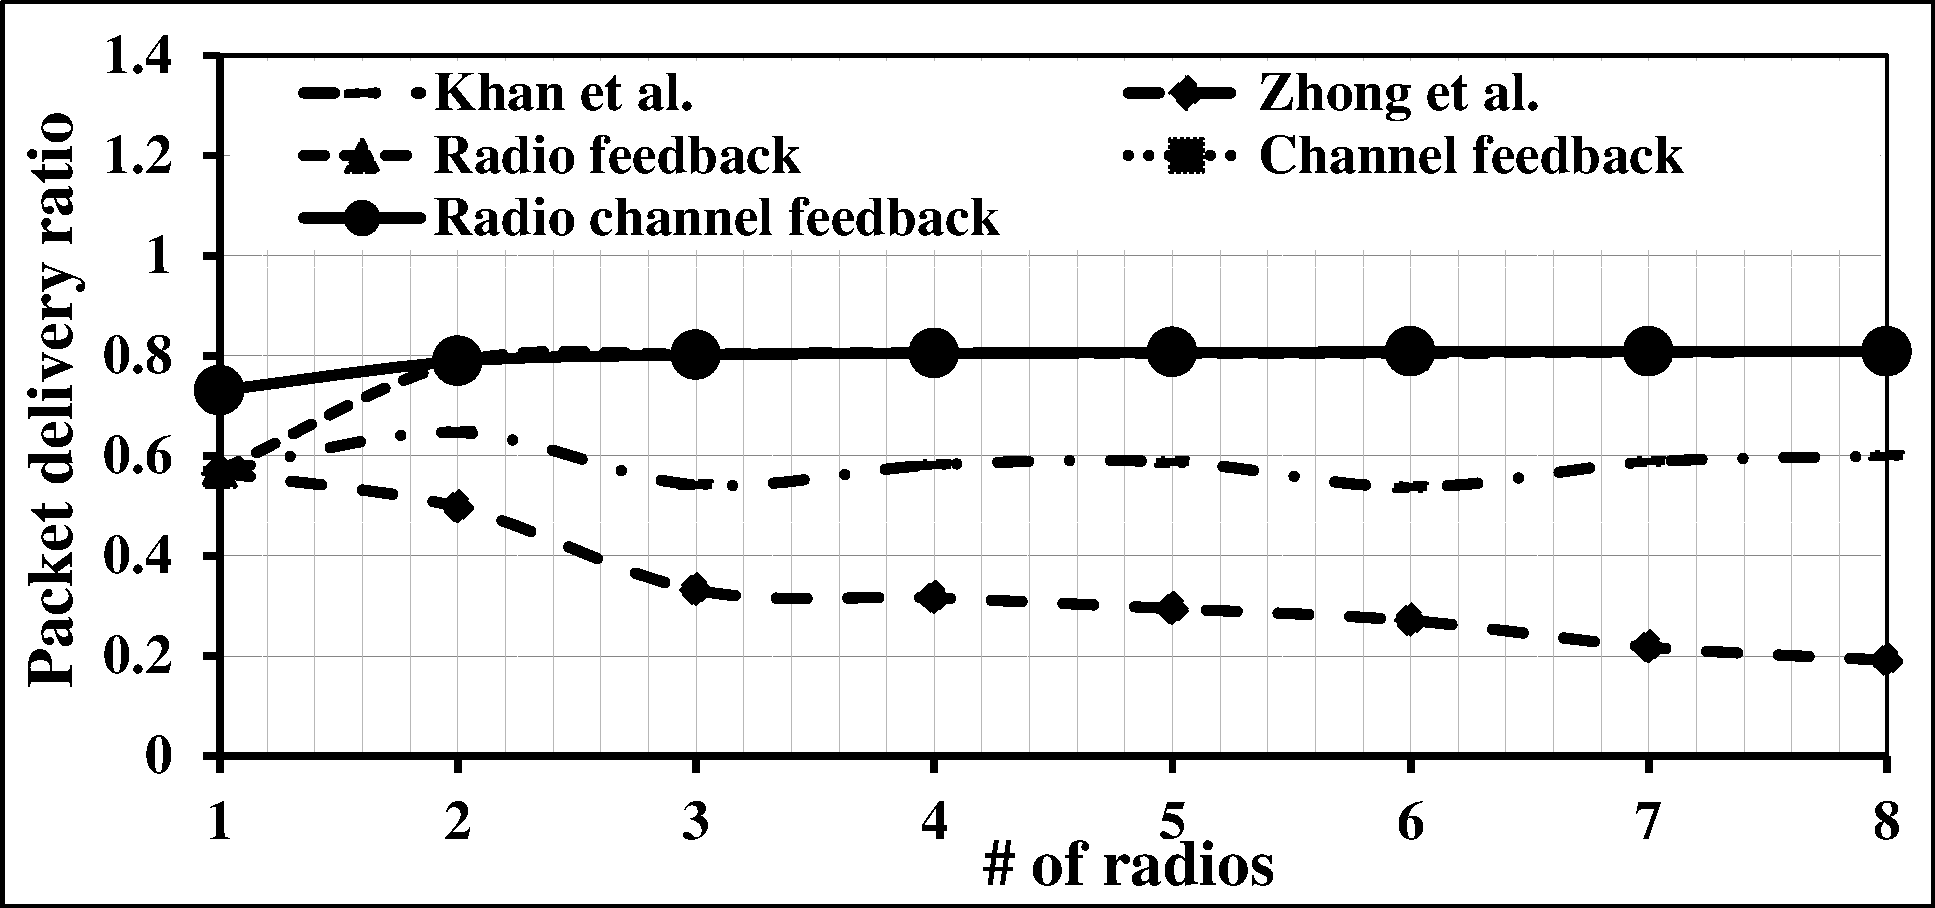
\includegraphics[width=\textwidth]{topology4/DeliveryRatio24d2}
        \caption{2Mbps application data rate}
        \label{fig:topology4PD2}
    \end{subfigure}
    ~\\
    \begin{subfigure}[t]{0.45\textwidth}
        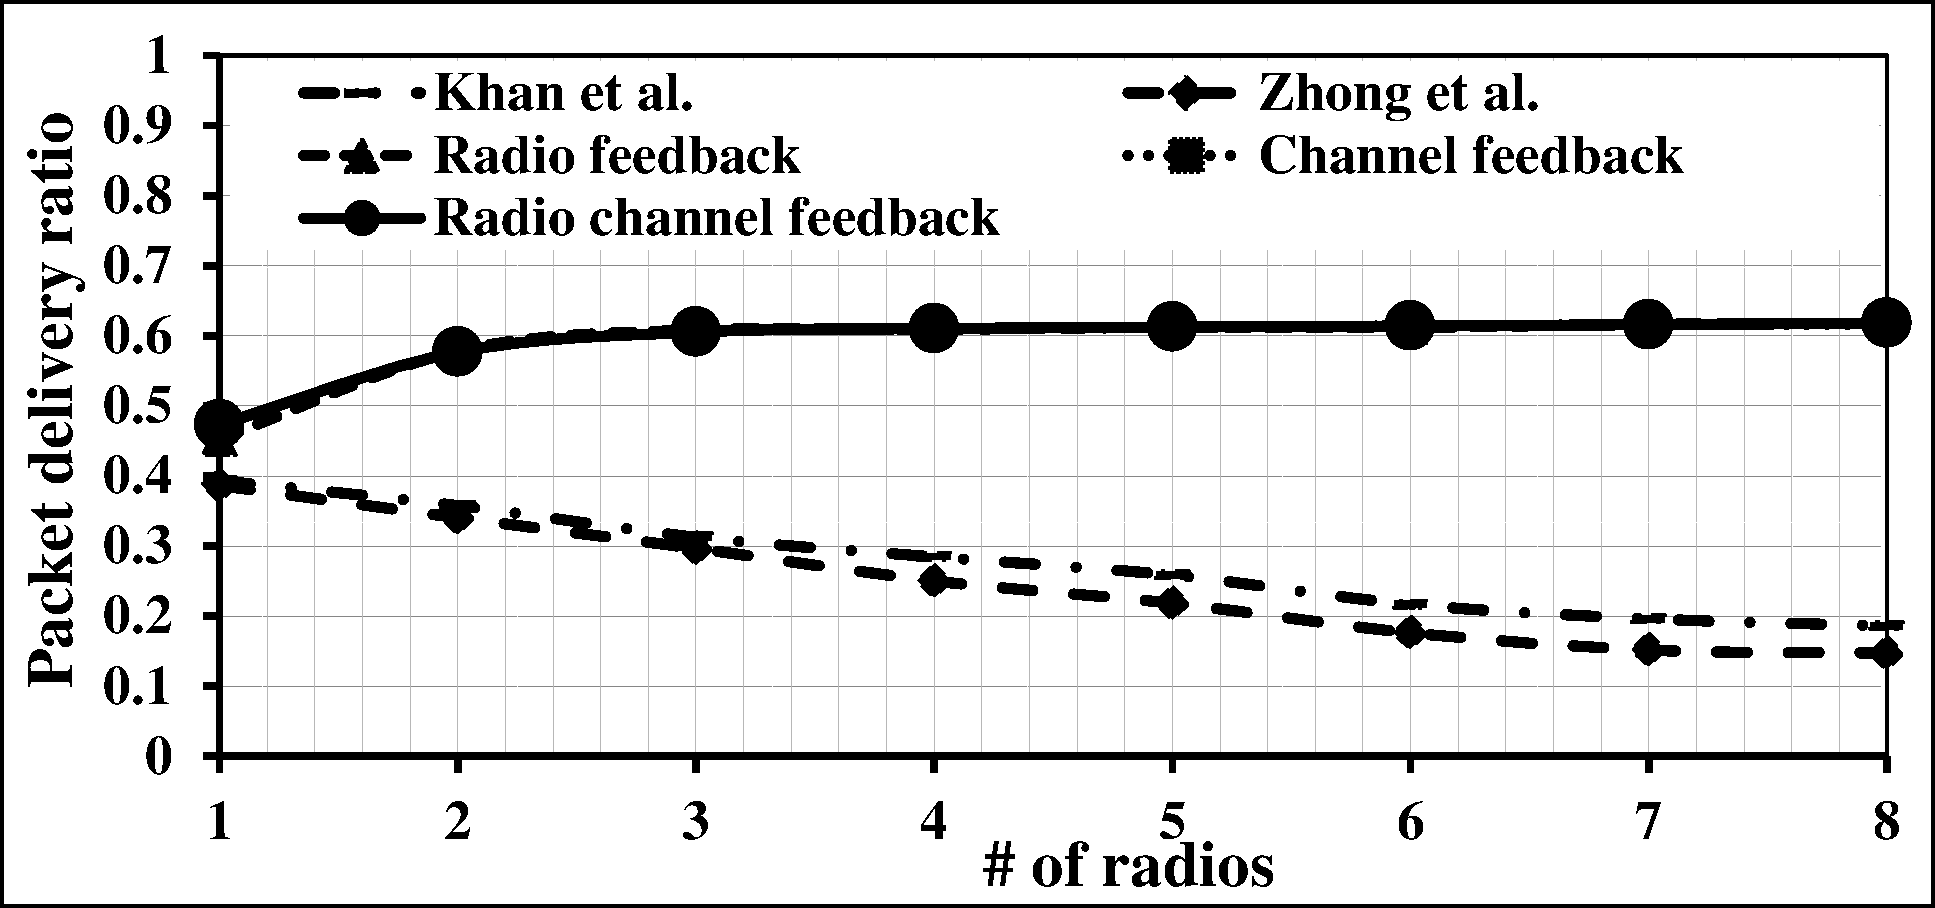
\includegraphics[width=\textwidth]{topology4/DeliveryRatio24d4}
        \caption{4Mbps application data rate}
        \label{fig:topology4PD3}
    \end{subfigure}
    ~
    \begin{subfigure}[t]{0.45\textwidth}
        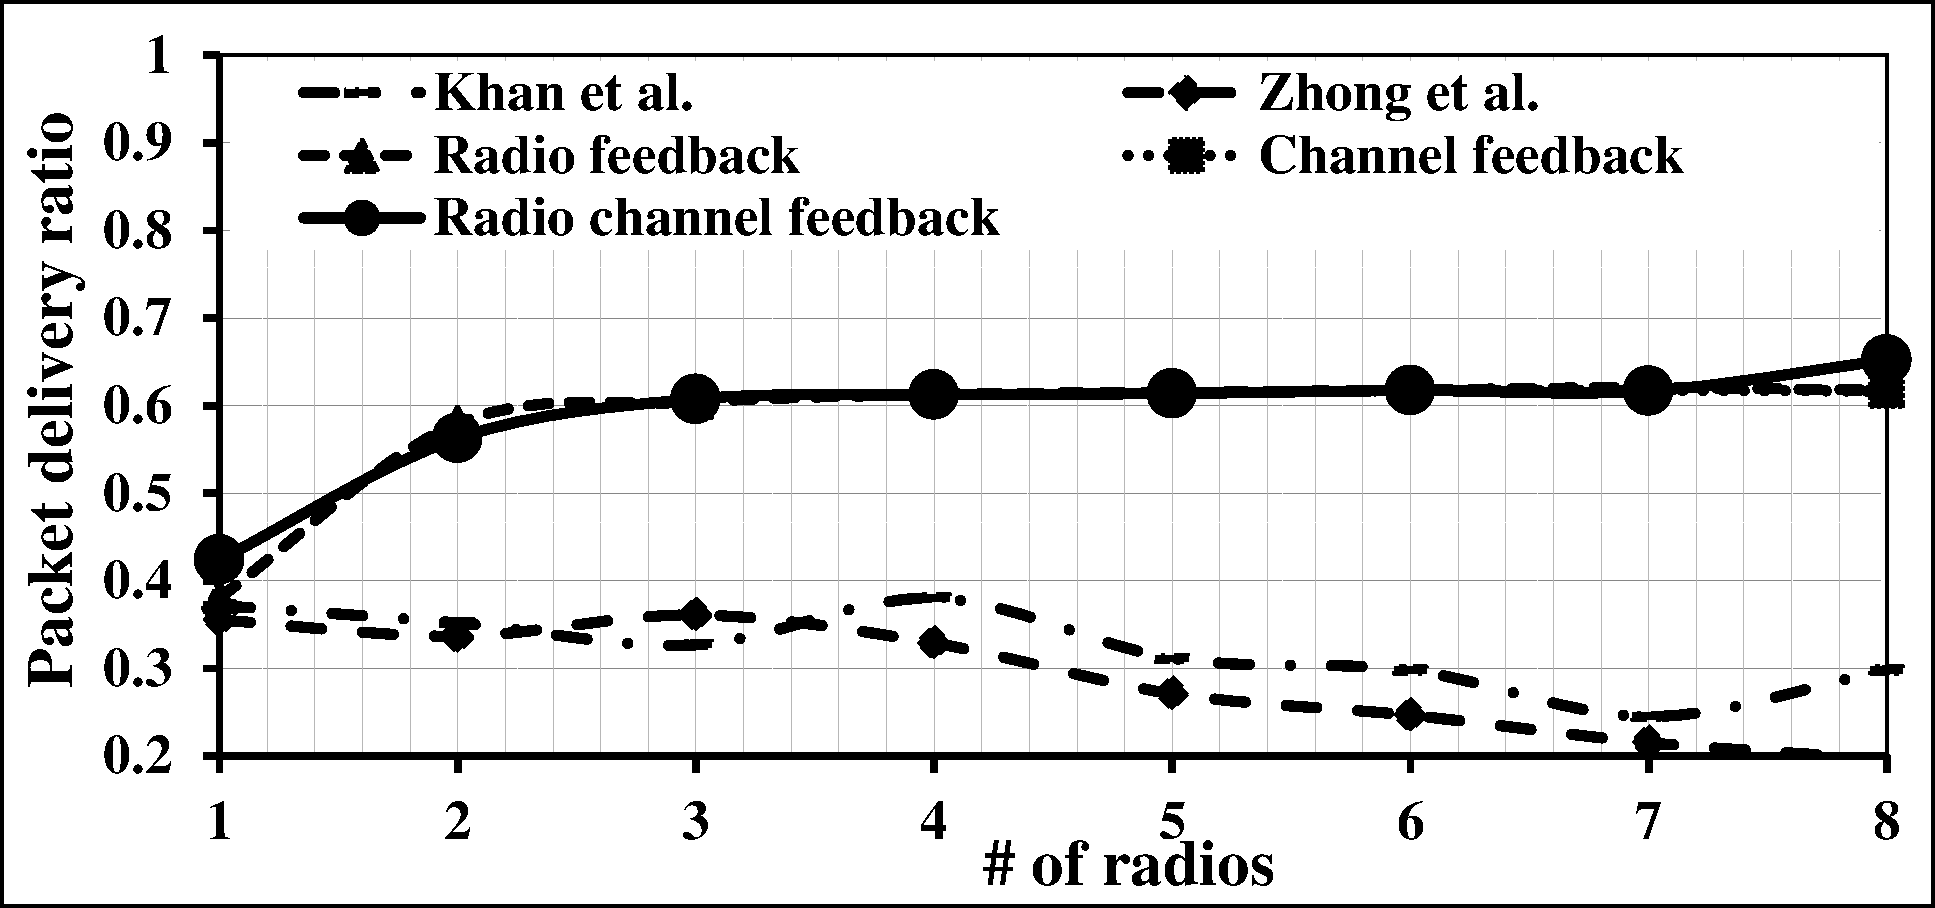
\includegraphics[width=\textwidth]{topology4/DeliveryRatio24d8}
        \caption{8Mbps application data rate}
        \label{fig:topology4PD4}
    \end{subfigure}
    ~\\
    \begin{subfigure}[t]{0.45\textwidth}
        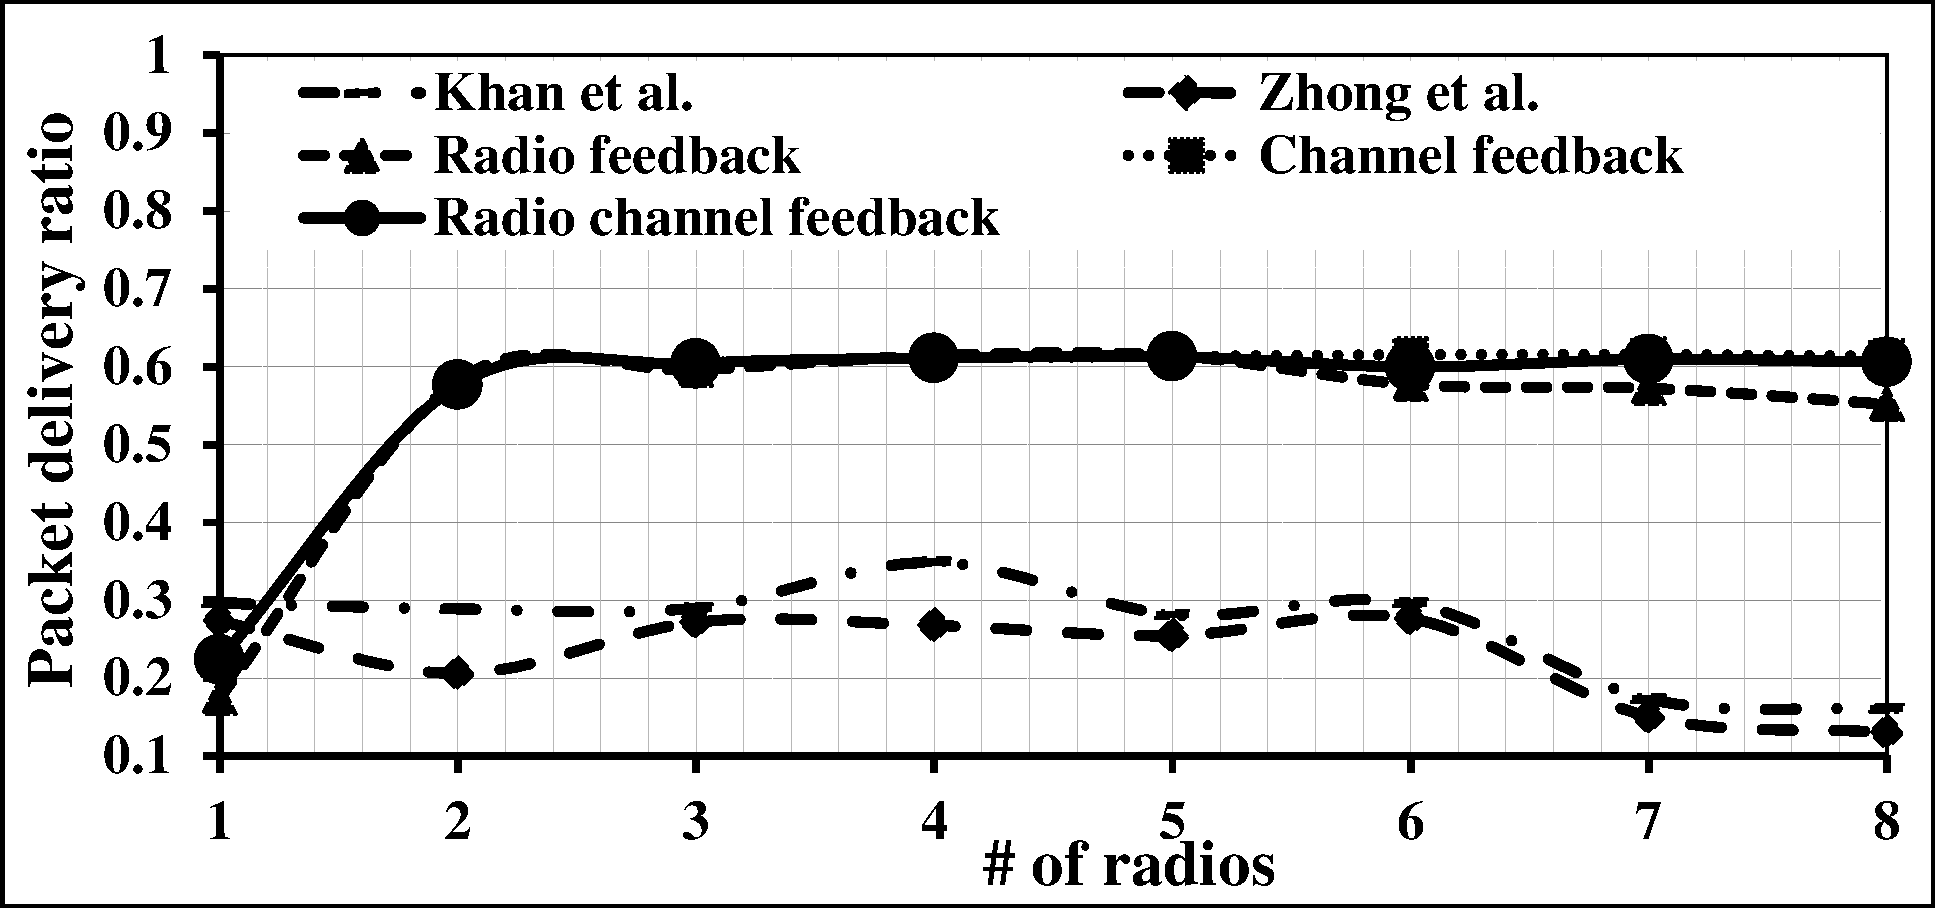
\includegraphics[width=\textwidth]{topology4/DeliveryRatio24d16}
        \caption{16Mbps application data rate}
        \label{fig:topology4PD5}
    \end{subfigure}
    ~
    \begin{subfigure}[t]{0.45\textwidth}
        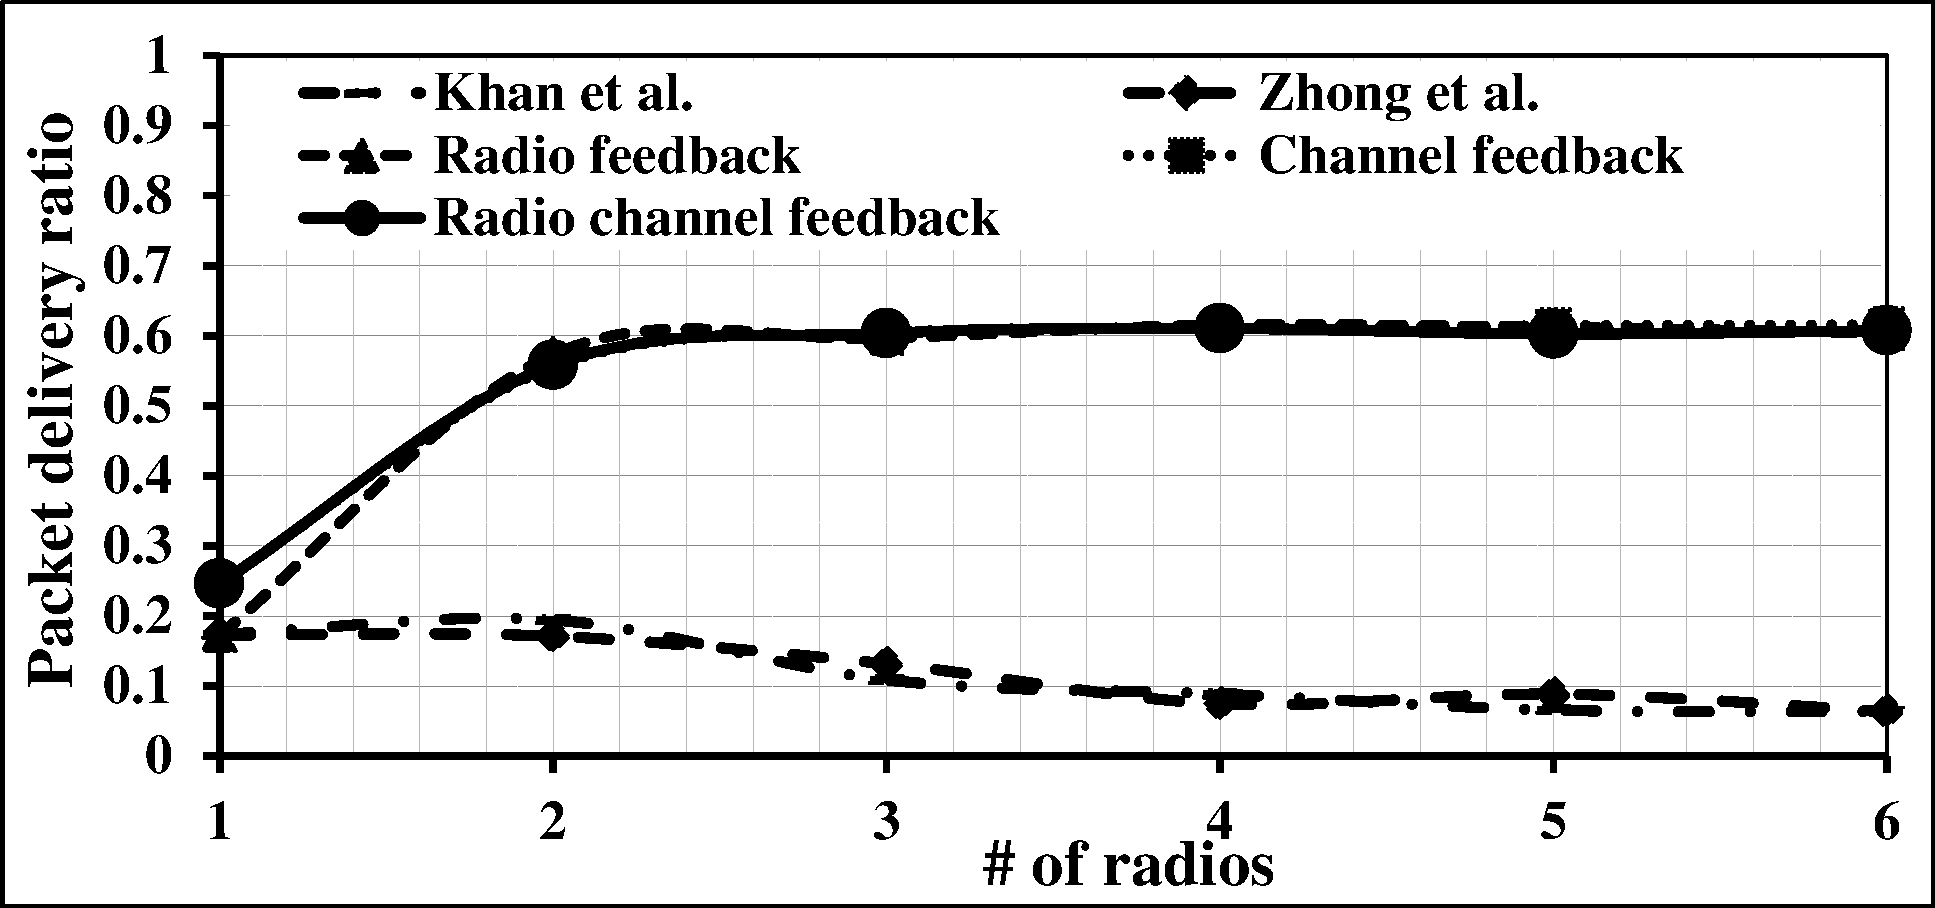
\includegraphics[width=\textwidth]{topology4/DeliveryRatio24d32}
        \caption{32Mbps application data rate}
        \label{fig:topology4PD6}
    \end{subfigure}
    \caption{Application layer packet delivery ratio with varying number of radios for various application data rates}
    \label{fig:topology4PD}
\end{figure*}



\begin{table}[!htb]
	\centering
    \caption{Performance improvement achieved using the radio feedback-based approach with respect to the approaches proposed by Khan et al.,~\cite{khan2015towards} and Zhong et al.,~\cite{zhong2014capacity}}
  \label{tab:topology4RadioImprovement}
  \renewcommand\multirowsetup{\centering}
    \begin{tabular}{|>{\centering} p{0.05\textwidth}|c|c|c|c|c|c|c|c|}
    \hline
    \multirow{2}{0.05\textwidth}{\newline \newline \newline Appli-\\cation data rate} & \multicolumn{2}{|p{0.08\textwidth}|}{\centering\% increase in throughput with respect to} & \multicolumn{2}{|p{0.08\textwidth}|}{\centering\% decrease in end-to-end delay with respect to} & \multicolumn{2}{|p{0.08\textwidth}|}{\centering\% decrease in packet drop ratio with respect to} & \multicolumn{2}{|p{0.08\textwidth}|}{\centering\% increase in application layer packet delivery ratio with respect to}\\
    \cline{2-9}
          & \multicolumn{1}{|p{0.025\textwidth}|}{\centering Khan et al.} & \multicolumn{1}{|p{0.025\textwidth}|}{\centering Zhong et al.} & \multicolumn{1}{|p{0.025\textwidth}|}{\centering Khan et al.} & \multicolumn{1}{|p{0.025\textwidth}|}{\centering Zhong et al.} & \multicolumn{1}{|p{0.03\textwidth}|}{\centering Khan et al.} & \multicolumn{1}{|p{0.025\textwidth}|}{\centering Zhong et al.} & \multicolumn{1}{|p{0.025\textwidth}|}{\centering Khan et al.} & \multicolumn{1}{|p{0.025\textwidth}|}{\centering Zhong et al.}\\
    \hline
    1Mbps & 55 & 14 & -9 & 48 & 57 & 57 & 12 & 12 \\\hline
    2Mbps & 64 & 33 & -10 & 50 & 52 & 54 & 24 & 27 \\\hline
    4Mbps & 66 & 44 & -16 & 45 & 40 & 41 & 52 & 52 \\\hline
    8Mbps & 63 & 46 & -17 & 32 & 26 & 26 & 42 & 43 \\\hline
    16Mbps & 62 & 48 & -16 & 24 & 18 & 18 & 40 & 46 \\\hline
    32Mbps & 63 & 42 & -13 & 28 & 13 & 12 & 69 & 73 \\\hline
    \end{tabular}%
\end{table}

\begin{table}[!htb]
	\centering
    \caption{Performance improvement achieved using the channel feedback-based approach with respect to the approaches proposed by Khan et al.,~\cite{khan2015towards} and Zhong et al.,~\cite{zhong2014capacity}}
  \label{tab:topology4ChannelImprovement}
  \renewcommand\multirowsetup{\centering}
    \begin{tabular}{|>{\centering} p{0.05\textwidth}|c|c|c|c|c|c|c|c|}
    \hline
    \multirow{2}{0.05\textwidth}{\newline \newline \newline Appli-\\cation data rate} & \multicolumn{2}{|p{0.08\textwidth}|}{\centering\% increase in throughput with respect to} & \multicolumn{2}{|p{0.08\textwidth}|}{\centering\% decrease in end-to-end delay with respect to} & \multicolumn{2}{|p{0.08\textwidth}|}{\centering\% decrease in packet drop ratio with respect to} & \multicolumn{2}{|p{0.08\textwidth}|}{\centering\% increase in application layer packet delivery ratio with respect to}\\
    \cline{2-9}
          & \multicolumn{1}{|p{0.025\textwidth}|}{\centering Khan et al.} & \multicolumn{1}{|p{0.025\textwidth}|}{\centering Zhong et al.} & \multicolumn{1}{|p{0.025\textwidth}|}{\centering Khan et al.} & \multicolumn{1}{|p{0.025\textwidth}|}{\centering Zhong et al.} & \multicolumn{1}{|p{0.03\textwidth}|}{\centering Khan et al.} & \multicolumn{1}{|p{0.025\textwidth}|}{\centering Zhong et al.} & \multicolumn{1}{|p{0.025\textwidth}|}{\centering Khan et al.} & \multicolumn{1}{|p{0.025\textwidth}|}{\centering Zhong et al.}\\
    \hline
    1Mbps & 55 & 15 & -8 & 49 & 58 & 58 & 12 & 41 \\\hline 
    2Mbps & 63 & 31 & -15 & 48 & 51 & 51 & 27 & 55 \\\hline 
    4Mbps & 66 & 44 & -11 & 42 & 40 & 38 & 52 & 52 \\\hline 
    8Mbps & 64 & 49 & -16 & 31 & 30 & 30 & 44 & 48\\\hline 
    16Mbps & 68 & 55 & -13 & 25 & 21 & 20 & 45 & 47 \\\hline 
    32Mbps & 64 & 44 & -16 & 23 & 15 & 15 & 73 & 68 \\\hline 
    \end{tabular}%
\end{table}

\begin{table}[!htb]
	\centering
    \caption{Performance improvement achieved using the radio channel feedback-based approach with respect to the approaches proposed by Khan et al.,~\cite{khan2015towards} and Zhong et al.,~\cite{zhong2014capacity}}
  \label{tab:topology4RadioChannelImprovement}
  \renewcommand\multirowsetup{\centering}
    \begin{tabular}{|>{\centering} p{0.05\textwidth}|c|c|c|c|c|c|c|c|}
    \hline
    \multirow{2}{0.05\textwidth}{\newline \newline \newline Appli-\\cation data rate} & \multicolumn{2}{|p{0.08\textwidth}|}{\centering\% increase in throughput with respect to} & \multicolumn{2}{|p{0.08\textwidth}|}{\centering\% decrease in end-to-end delay with respect to} & \multicolumn{2}{|p{0.08\textwidth}|}{\centering\% decrease in packet drop ratio with respect to} & \multicolumn{2}{|p{0.08\textwidth}|}{\centering\% increase in application layer packet delivery ratio with respect to}\\
    \cline{2-9}
          & \multicolumn{1}{|p{0.025\textwidth}|}{\centering Khan et al.} & \multicolumn{1}{|p{0.025\textwidth}|}{\centering Zhong et al.} & \multicolumn{1}{|p{0.025\textwidth}|}{\centering Khan et al.} & \multicolumn{1}{|p{0.025\textwidth}|}{\centering Zhong et al.} & \multicolumn{1}{|p{0.03\textwidth}|}{\centering Khan et al.} & \multicolumn{1}{|p{0.025\textwidth}|}{\centering Zhong et al.} & \multicolumn{1}{|p{0.025\textwidth}|}{\centering Khan et al.} & \multicolumn{1}{|p{0.025\textwidth}|}{\centering Zhong et al.}\\
    \hline 
    1Mbps & 55 & 15 & -18 & 49 & 58 & 58 & 42 & 42 \\\hline 
    2Mbps & 63 & 31 & -15 & 49 & 51 & 51 & 58 & 58 \\\hline 
    4Mbps & 66 & 44 & -17 & 42 & 40 & 41 & 57 & 57 \\\hline 
    8Mbps & 63 & 49 & -17 & 31 & 29 & 30 & 49 & 50 \\\hline 
    16Mbps & 68 & 55 & -14 & 27 & 21 & 20 & 53 & 52 \\\hline 
    32Mbps & 64 & 43 & -13 & 23 & 15 & 15 & 73 & 73 \\\hline 
    \end{tabular}%
    \vspace{-0.625cm}
\end{table}


\iffalse
% Table generated by Excel2LaTeX from sheet 'Sheet1'
\begin{table*}[!htbp]
  \centering
  \caption{Percentage improvement achieved using the feedback-based approach with respect to the approaches proposed by Khan et al.,~\cite{khan2015towards} and Zhong et al.,~\cite{zhong2014capacity}}
  \label{tab:topology4Improvement}
    \begin{tabular}{ccccccc}
    \toprule
    \multirow{2}[0]{*}{Application data rate} & \multicolumn{2}{p{0.2\textwidth}}{\% increase in total network througput w.r.t} & \multicolumn{2}{p{0.2\textwidth}}{\% decrease in per packet end-to-end delay w.r.t} & \multicolumn{2}{p{0.2\textwidth}}{\% decrease in packet drop ratio w.r.t} \\
          & \multicolumn{1}{l}{Khan et al.} & \multicolumn{1}{l}{Zhong et al.} & \multicolumn{1}{l}{Khan et al.} & \multicolumn{1}{l}{Zhong et al.} & \multicolumn{1}{l}{Khan et al.} & \multicolumn{1}{l}{Zhong et al.} \\
    \midrule
    1Mbps & 55.862076 & 16.77937765 & -15.155181 & 50.73693391 & 59.865701 & 59.8842253 \\
    2Mbps & 64.74406156 & 33.88792815 & -17.680018 & 51.43200614 & 53.816642 & 53.5899378 \\
    4Mbps & 67.37679147 & 45.85754947 & -30.950717 & 45.37420031 & 41.190572 & 41.8005298 \\
    8Mbps & 65.2701612 & 49.89498939 & -36.956627 & 33.28484049 & 29.774189 & 29.9230113 \\
    16Mbps & 68.48584166 & 55.17376536 & -24.008348 & 28.92168644 & 21.287883 & 20.6884369 \\
    32Mbps & 65.62299103 & 45.56263021 & -13.078491 & 28.3215896 & 15.364822 & 14.5973083 \\
    \bottomrule
    \end{tabular}%
\end{table*}%
\fi


\section{Simulation Findings}

Though we have performed discrete event simulations for various network topologies varying the number of secondary users from 12 to 40 with a granularity of 4, in this thesis, due to space limitation, we have presented the simulation results for only one topology with 24 secondary users. Appendix~\ref{app:allTopologies} of this thesis contains the other results. Here, our proposed approach for MRCRNs obtains similar simulation results in case of other seven network topologies as well. Based on these simulation results, we obtain the following findings:

\begin{itemize}
    \item Over all these topologies, our proposed feedback-based approach improves total network throughput by 51\% on an average against that of existing approaches.
    \item Over all these topologies, our proposed feedback-based approach decreases packet drop ratio by 35\% on an average against that of existing approaches.
    \item Among three variants of our proposed feedback-based approach, radio channel feedback approach marginally (3\%) performs better over the other variants.
    \item For MRCRNs, our proposed feedback-based approach increases throughput with an increase in the number of radios for low to medium (1 -- 8Mbps) data rates. For high data rates (16 -- 32 Mbps), multiple radio introduction could not make significant impact on throughput and throughput usually degrades with an increase in the number of radios.
    \item For MRCRNs, our proposed feedback-based approach is able to make average end-to-end delay almost constant with an increase in the number of radios for low to medium (1 -- 8Mbps) data rates. For high data rates (16 -- 32 Mbps), delay usually increases with an increase in the number of radios.
    \item For MRCRNs, our proposed feedback-based approach improves average packet drop ratio with an increase in the number of radios for low to medium (1 -- 16Mbps) data rates. For high data rate (32 Mbps), packet drop ratio remains constant with an increase in the number of radios.
\end{itemize}

\endinput
